\documentclass[twoside]{book}

% Packages required by doxygen
\usepackage{fixltx2e}
\usepackage{calc}
\usepackage{doxygen}
\usepackage[export]{adjustbox} % also loads graphicx
\usepackage{graphicx}
\usepackage[utf8]{inputenc}
\usepackage{makeidx}
\usepackage{multicol}
\usepackage{multirow}
\PassOptionsToPackage{warn}{textcomp}
\usepackage{textcomp}
\usepackage[nointegrals]{wasysym}
\usepackage[table]{xcolor}

% Font selection
\usepackage[T1]{fontenc}
\usepackage[scaled=.90]{helvet}
\usepackage{courier}
\usepackage{amssymb}
\usepackage{sectsty}
\renewcommand{\familydefault}{\sfdefault}
\allsectionsfont{%
  \fontseries{bc}\selectfont%
  \color{darkgray}%
}
\renewcommand{\DoxyLabelFont}{%
  \fontseries{bc}\selectfont%
  \color{darkgray}%
}
\newcommand{\+}{\discretionary{\mbox{\scriptsize$\hookleftarrow$}}{}{}}

% Page & text layout
\usepackage{geometry}
\geometry{%
  a4paper,%
  top=2.5cm,%
  bottom=2.5cm,%
  left=2.5cm,%
  right=2.5cm%
}
\tolerance=750
\hfuzz=15pt
\hbadness=750
\setlength{\emergencystretch}{15pt}
\setlength{\parindent}{0cm}
\setlength{\parskip}{3ex plus 2ex minus 2ex}
\makeatletter
\renewcommand{\paragraph}{%
  \@startsection{paragraph}{4}{0ex}{-1.0ex}{1.0ex}{%
    \normalfont\normalsize\bfseries\SS@parafont%
  }%
}
\renewcommand{\subparagraph}{%
  \@startsection{subparagraph}{5}{0ex}{-1.0ex}{1.0ex}{%
    \normalfont\normalsize\bfseries\SS@subparafont%
  }%
}
\makeatother

% Headers & footers
\usepackage{fancyhdr}
\pagestyle{fancyplain}
\fancyhead[LE]{\fancyplain{}{\bfseries\thepage}}
\fancyhead[CE]{\fancyplain{}{}}
\fancyhead[RE]{\fancyplain{}{\bfseries\leftmark}}
\fancyhead[LO]{\fancyplain{}{\bfseries\rightmark}}
\fancyhead[CO]{\fancyplain{}{}}
\fancyhead[RO]{\fancyplain{}{\bfseries\thepage}}
\fancyfoot[LE]{\fancyplain{}{}}
\fancyfoot[CE]{\fancyplain{}{}}
\fancyfoot[RE]{\fancyplain{}{\bfseries\scriptsize Generated by Doxygen }}
\fancyfoot[LO]{\fancyplain{}{\bfseries\scriptsize Generated by Doxygen }}
\fancyfoot[CO]{\fancyplain{}{}}
\fancyfoot[RO]{\fancyplain{}{}}
\renewcommand{\footrulewidth}{0.4pt}
\renewcommand{\chaptermark}[1]{%
  \markboth{#1}{}%
}
\renewcommand{\sectionmark}[1]{%
  \markright{\thesection\ #1}%
}

% Indices & bibliography
\usepackage{natbib}
\usepackage[titles]{tocloft}
\setcounter{tocdepth}{3}
\setcounter{secnumdepth}{5}
\makeindex

% Hyperlinks (required, but should be loaded last)
\usepackage{ifpdf}
\ifpdf
  \usepackage[pdftex,pagebackref=true]{hyperref}
\else
  \usepackage[ps2pdf,pagebackref=true]{hyperref}
\fi
\hypersetup{%
  colorlinks=true,%
  linkcolor=blue,%
  citecolor=blue,%
  unicode%
}

% Custom commands
\newcommand{\clearemptydoublepage}{%
  \newpage{\pagestyle{empty}\cleardoublepage}%
}

\usepackage{caption}
\captionsetup{labelsep=space,justification=centering,font={bf},singlelinecheck=off,skip=4pt,position=top}

%===== C O N T E N T S =====

\begin{document}

% Titlepage & ToC
\hypersetup{pageanchor=false,
             bookmarksnumbered=true,
             pdfencoding=unicode
            }
\pagenumbering{alph}
\begin{titlepage}
\vspace*{7cm}
\begin{center}%
{\Large Exp\+\_\+assignment2 }\\
\vspace*{1cm}
{\large Generated by Doxygen 1.8.13}\\
\end{center}
\end{titlepage}
\clearemptydoublepage
\pagenumbering{roman}
\tableofcontents
\clearemptydoublepage
\pagenumbering{arabic}
\hypersetup{pageanchor=true}

%--- Begin generated contents ---
\chapter{Hierarchical Index}
\section{Class Hierarchy}
This inheritance list is sorted roughly, but not completely, alphabetically\+:\begin{DoxyCompactList}
\item \contentsline{section}{robot\+\_\+to\+\_\+ball.\+image\+\_\+feature}{\pageref{classrobot__to__ball_1_1image__feature}}{}
\item \contentsline{section}{state\+\_\+machine.\+image\+\_\+feature}{\pageref{classstate__machine_1_1image__feature}}{}
\item State\begin{DoxyCompactList}
\item \contentsline{section}{state\+\_\+machine.\+Normal}{\pageref{classstate__machine_1_1Normal}}{}
\item \contentsline{section}{state\+\_\+machine.\+Play}{\pageref{classstate__machine_1_1Play}}{}
\item \contentsline{section}{state\+\_\+machine.\+Sleep}{\pageref{classstate__machine_1_1Sleep}}{}
\end{DoxyCompactList}
\end{DoxyCompactList}

\chapter{Class Index}
\section{Class List}
Here are the classes, structs, unions and interfaces with brief descriptions\+:\begin{DoxyCompactList}
\item\contentsline{section}{\hyperlink{structros_1_1service__traits_1_1DataType_3_01_1_1ass1_1_1pos__service_01_4}{ros\+::service\+\_\+traits\+::\+Data\+Type$<$ \+::ass1\+::pos\+\_\+service $>$} }{\pageref{structros_1_1service__traits_1_1DataType_3_01_1_1ass1_1_1pos__service_01_4}}{}
\item\contentsline{section}{\hyperlink{structros_1_1service__traits_1_1DataType_3_01_1_1ass1_1_1pos__serviceRequest_01_4}{ros\+::service\+\_\+traits\+::\+Data\+Type$<$ \+::ass1\+::pos\+\_\+service\+Request $>$} }{\pageref{structros_1_1service__traits_1_1DataType_3_01_1_1ass1_1_1pos__serviceRequest_01_4}}{}
\item\contentsline{section}{\hyperlink{structros_1_1message__traits_1_1DataType_3_01_1_1ass1_1_1pos__serviceRequest___3_01ContainerAllocator_01_4_01_4}{ros\+::message\+\_\+traits\+::\+Data\+Type$<$ \+::ass1\+::pos\+\_\+service\+Request\+\_\+$<$ Container\+Allocator $>$ $>$} }{\pageref{structros_1_1message__traits_1_1DataType_3_01_1_1ass1_1_1pos__serviceRequest___3_01ContainerAllocator_01_4_01_4}}{}
\item\contentsline{section}{\hyperlink{structros_1_1service__traits_1_1DataType_3_01_1_1ass1_1_1pos__serviceResponse_01_4}{ros\+::service\+\_\+traits\+::\+Data\+Type$<$ \+::ass1\+::pos\+\_\+service\+Response $>$} }{\pageref{structros_1_1service__traits_1_1DataType_3_01_1_1ass1_1_1pos__serviceResponse_01_4}}{}
\item\contentsline{section}{\hyperlink{structros_1_1message__traits_1_1DataType_3_01_1_1ass1_1_1pos__serviceResponse___3_01ContainerAllocator_01_4_01_4}{ros\+::message\+\_\+traits\+::\+Data\+Type$<$ \+::ass1\+::pos\+\_\+service\+Response\+\_\+$<$ Container\+Allocator $>$ $>$} }{\pageref{structros_1_1message__traits_1_1DataType_3_01_1_1ass1_1_1pos__serviceResponse___3_01ContainerAllocator_01_4_01_4}}{}
\item\contentsline{section}{\hyperlink{structros_1_1message__traits_1_1DataType_3_01_1_1exp__assignment2_1_1PlanningAction___3_01ContainerAllocator_01_4_01_4}{ros\+::message\+\_\+traits\+::\+Data\+Type$<$ \+::exp\+\_\+assignment2\+::\+Planning\+Action\+\_\+$<$ Container\+Allocator $>$ $>$} }{\pageref{structros_1_1message__traits_1_1DataType_3_01_1_1exp__assignment2_1_1PlanningAction___3_01ContainerAllocator_01_4_01_4}}{}
\item\contentsline{section}{\hyperlink{structros_1_1message__traits_1_1DataType_3_01_1_1exp__assignment2_1_1PlanningActionFeedback___3_01ContainerAllocator_01_4_01_4}{ros\+::message\+\_\+traits\+::\+Data\+Type$<$ \+::exp\+\_\+assignment2\+::\+Planning\+Action\+Feedback\+\_\+$<$ Container\+Allocator $>$ $>$} }{\pageref{structros_1_1message__traits_1_1DataType_3_01_1_1exp__assignment2_1_1PlanningActionFeedback___3_01ContainerAllocator_01_4_01_4}}{}
\item\contentsline{section}{\hyperlink{structros_1_1message__traits_1_1DataType_3_01_1_1exp__assignment2_1_1PlanningActionGoal___3_01ContainerAllocator_01_4_01_4}{ros\+::message\+\_\+traits\+::\+Data\+Type$<$ \+::exp\+\_\+assignment2\+::\+Planning\+Action\+Goal\+\_\+$<$ Container\+Allocator $>$ $>$} }{\pageref{structros_1_1message__traits_1_1DataType_3_01_1_1exp__assignment2_1_1PlanningActionGoal___3_01ContainerAllocator_01_4_01_4}}{}
\item\contentsline{section}{\hyperlink{structros_1_1message__traits_1_1DataType_3_01_1_1exp__assignment2_1_1PlanningActionResult___3_01ContainerAllocator_01_4_01_4}{ros\+::message\+\_\+traits\+::\+Data\+Type$<$ \+::exp\+\_\+assignment2\+::\+Planning\+Action\+Result\+\_\+$<$ Container\+Allocator $>$ $>$} }{\pageref{structros_1_1message__traits_1_1DataType_3_01_1_1exp__assignment2_1_1PlanningActionResult___3_01ContainerAllocator_01_4_01_4}}{}
\item\contentsline{section}{\hyperlink{structros_1_1message__traits_1_1DataType_3_01_1_1exp__assignment2_1_1PlanningFeedback___3_01ContainerAllocator_01_4_01_4}{ros\+::message\+\_\+traits\+::\+Data\+Type$<$ \+::exp\+\_\+assignment2\+::\+Planning\+Feedback\+\_\+$<$ Container\+Allocator $>$ $>$} }{\pageref{structros_1_1message__traits_1_1DataType_3_01_1_1exp__assignment2_1_1PlanningFeedback___3_01ContainerAllocator_01_4_01_4}}{}
\item\contentsline{section}{\hyperlink{structros_1_1message__traits_1_1DataType_3_01_1_1exp__assignment2_1_1PlanningGoal___3_01ContainerAllocator_01_4_01_4}{ros\+::message\+\_\+traits\+::\+Data\+Type$<$ \+::exp\+\_\+assignment2\+::\+Planning\+Goal\+\_\+$<$ Container\+Allocator $>$ $>$} }{\pageref{structros_1_1message__traits_1_1DataType_3_01_1_1exp__assignment2_1_1PlanningGoal___3_01ContainerAllocator_01_4_01_4}}{}
\item\contentsline{section}{\hyperlink{structros_1_1message__traits_1_1DataType_3_01_1_1exp__assignment2_1_1PlanningResult___3_01ContainerAllocator_01_4_01_4}{ros\+::message\+\_\+traits\+::\+Data\+Type$<$ \+::exp\+\_\+assignment2\+::\+Planning\+Result\+\_\+$<$ Container\+Allocator $>$ $>$} }{\pageref{structros_1_1message__traits_1_1DataType_3_01_1_1exp__assignment2_1_1PlanningResult___3_01ContainerAllocator_01_4_01_4}}{}
\item\contentsline{section}{\hyperlink{structros_1_1message__traits_1_1DataType_3_01_1_1learning__actionlib_1_1FibonacciAction___3_01ContainerAllocator_01_4_01_4}{ros\+::message\+\_\+traits\+::\+Data\+Type$<$ \+::learning\+\_\+actionlib\+::\+Fibonacci\+Action\+\_\+$<$ Container\+Allocator $>$ $>$} }{\pageref{structros_1_1message__traits_1_1DataType_3_01_1_1learning__actionlib_1_1FibonacciAction___3_01ContainerAllocator_01_4_01_4}}{}
\item\contentsline{section}{\hyperlink{structros_1_1message__traits_1_1DataType_3_01_1_1learning__actionlib_1_1FibonacciActionFeedback_4b5000ca73b59c79b63e13e37ac0341d}{ros\+::message\+\_\+traits\+::\+Data\+Type$<$ \+::learning\+\_\+actionlib\+::\+Fibonacci\+Action\+Feedback\+\_\+$<$ Container\+Allocator $>$ $>$} }{\pageref{structros_1_1message__traits_1_1DataType_3_01_1_1learning__actionlib_1_1FibonacciActionFeedback_4b5000ca73b59c79b63e13e37ac0341d}}{}
\item\contentsline{section}{\hyperlink{structros_1_1message__traits_1_1DataType_3_01_1_1learning__actionlib_1_1FibonacciActionGoal___3_01ContainerAllocator_01_4_01_4}{ros\+::message\+\_\+traits\+::\+Data\+Type$<$ \+::learning\+\_\+actionlib\+::\+Fibonacci\+Action\+Goal\+\_\+$<$ Container\+Allocator $>$ $>$} }{\pageref{structros_1_1message__traits_1_1DataType_3_01_1_1learning__actionlib_1_1FibonacciActionGoal___3_01ContainerAllocator_01_4_01_4}}{}
\item\contentsline{section}{\hyperlink{structros_1_1message__traits_1_1DataType_3_01_1_1learning__actionlib_1_1FibonacciActionResult___7dcb5a3074c9ee8e9d1bacdcd8ac1ad5}{ros\+::message\+\_\+traits\+::\+Data\+Type$<$ \+::learning\+\_\+actionlib\+::\+Fibonacci\+Action\+Result\+\_\+$<$ Container\+Allocator $>$ $>$} }{\pageref{structros_1_1message__traits_1_1DataType_3_01_1_1learning__actionlib_1_1FibonacciActionResult___7dcb5a3074c9ee8e9d1bacdcd8ac1ad5}}{}
\item\contentsline{section}{\hyperlink{structros_1_1message__traits_1_1DataType_3_01_1_1learning__actionlib_1_1FibonacciFeedback___3_01ContainerAllocator_01_4_01_4}{ros\+::message\+\_\+traits\+::\+Data\+Type$<$ \+::learning\+\_\+actionlib\+::\+Fibonacci\+Feedback\+\_\+$<$ Container\+Allocator $>$ $>$} }{\pageref{structros_1_1message__traits_1_1DataType_3_01_1_1learning__actionlib_1_1FibonacciFeedback___3_01ContainerAllocator_01_4_01_4}}{}
\item\contentsline{section}{\hyperlink{structros_1_1message__traits_1_1DataType_3_01_1_1learning__actionlib_1_1FibonacciGoal___3_01ContainerAllocator_01_4_01_4}{ros\+::message\+\_\+traits\+::\+Data\+Type$<$ \+::learning\+\_\+actionlib\+::\+Fibonacci\+Goal\+\_\+$<$ Container\+Allocator $>$ $>$} }{\pageref{structros_1_1message__traits_1_1DataType_3_01_1_1learning__actionlib_1_1FibonacciGoal___3_01ContainerAllocator_01_4_01_4}}{}
\item\contentsline{section}{\hyperlink{structros_1_1message__traits_1_1DataType_3_01_1_1learning__actionlib_1_1FibonacciResult___3_01ContainerAllocator_01_4_01_4}{ros\+::message\+\_\+traits\+::\+Data\+Type$<$ \+::learning\+\_\+actionlib\+::\+Fibonacci\+Result\+\_\+$<$ Container\+Allocator $>$ $>$} }{\pageref{structros_1_1message__traits_1_1DataType_3_01_1_1learning__actionlib_1_1FibonacciResult___3_01ContainerAllocator_01_4_01_4}}{}
\item\contentsline{section}{\hyperlink{structros_1_1message__traits_1_1DataType_3_01_1_1motion__plan_1_1PlanningAction___3_01ContainerAllocator_01_4_01_4}{ros\+::message\+\_\+traits\+::\+Data\+Type$<$ \+::motion\+\_\+plan\+::\+Planning\+Action\+\_\+$<$ Container\+Allocator $>$ $>$} }{\pageref{structros_1_1message__traits_1_1DataType_3_01_1_1motion__plan_1_1PlanningAction___3_01ContainerAllocator_01_4_01_4}}{}
\item\contentsline{section}{\hyperlink{structros_1_1message__traits_1_1DataType_3_01_1_1motion__plan_1_1PlanningActionFeedback___3_01ContainerAllocator_01_4_01_4}{ros\+::message\+\_\+traits\+::\+Data\+Type$<$ \+::motion\+\_\+plan\+::\+Planning\+Action\+Feedback\+\_\+$<$ Container\+Allocator $>$ $>$} }{\pageref{structros_1_1message__traits_1_1DataType_3_01_1_1motion__plan_1_1PlanningActionFeedback___3_01ContainerAllocator_01_4_01_4}}{}
\item\contentsline{section}{\hyperlink{structros_1_1message__traits_1_1DataType_3_01_1_1motion__plan_1_1PlanningActionGoal___3_01ContainerAllocator_01_4_01_4}{ros\+::message\+\_\+traits\+::\+Data\+Type$<$ \+::motion\+\_\+plan\+::\+Planning\+Action\+Goal\+\_\+$<$ Container\+Allocator $>$ $>$} }{\pageref{structros_1_1message__traits_1_1DataType_3_01_1_1motion__plan_1_1PlanningActionGoal___3_01ContainerAllocator_01_4_01_4}}{}
\item\contentsline{section}{\hyperlink{structros_1_1message__traits_1_1DataType_3_01_1_1motion__plan_1_1PlanningActionResult___3_01ContainerAllocator_01_4_01_4}{ros\+::message\+\_\+traits\+::\+Data\+Type$<$ \+::motion\+\_\+plan\+::\+Planning\+Action\+Result\+\_\+$<$ Container\+Allocator $>$ $>$} }{\pageref{structros_1_1message__traits_1_1DataType_3_01_1_1motion__plan_1_1PlanningActionResult___3_01ContainerAllocator_01_4_01_4}}{}
\item\contentsline{section}{\hyperlink{structros_1_1message__traits_1_1DataType_3_01_1_1motion__plan_1_1PlanningFeedback___3_01ContainerAllocator_01_4_01_4}{ros\+::message\+\_\+traits\+::\+Data\+Type$<$ \+::motion\+\_\+plan\+::\+Planning\+Feedback\+\_\+$<$ Container\+Allocator $>$ $>$} }{\pageref{structros_1_1message__traits_1_1DataType_3_01_1_1motion__plan_1_1PlanningFeedback___3_01ContainerAllocator_01_4_01_4}}{}
\item\contentsline{section}{\hyperlink{structros_1_1message__traits_1_1DataType_3_01_1_1motion__plan_1_1PlanningGoal___3_01ContainerAllocator_01_4_01_4}{ros\+::message\+\_\+traits\+::\+Data\+Type$<$ \+::motion\+\_\+plan\+::\+Planning\+Goal\+\_\+$<$ Container\+Allocator $>$ $>$} }{\pageref{structros_1_1message__traits_1_1DataType_3_01_1_1motion__plan_1_1PlanningGoal___3_01ContainerAllocator_01_4_01_4}}{}
\item\contentsline{section}{\hyperlink{structros_1_1message__traits_1_1DataType_3_01_1_1motion__plan_1_1PlanningResult___3_01ContainerAllocator_01_4_01_4}{ros\+::message\+\_\+traits\+::\+Data\+Type$<$ \+::motion\+\_\+plan\+::\+Planning\+Result\+\_\+$<$ Container\+Allocator $>$ $>$} }{\pageref{structros_1_1message__traits_1_1DataType_3_01_1_1motion__plan_1_1PlanningResult___3_01ContainerAllocator_01_4_01_4}}{}
\item\contentsline{section}{\hyperlink{structros_1_1service__traits_1_1DataType_3_01_1_1pos__server_1_1pos__service_01_4}{ros\+::service\+\_\+traits\+::\+Data\+Type$<$ \+::pos\+\_\+server\+::pos\+\_\+service $>$} }{\pageref{structros_1_1service__traits_1_1DataType_3_01_1_1pos__server_1_1pos__service_01_4}}{}
\item\contentsline{section}{\hyperlink{structros_1_1service__traits_1_1DataType_3_01_1_1pos__server_1_1pos__serviceRequest_01_4}{ros\+::service\+\_\+traits\+::\+Data\+Type$<$ \+::pos\+\_\+server\+::pos\+\_\+service\+Request $>$} }{\pageref{structros_1_1service__traits_1_1DataType_3_01_1_1pos__server_1_1pos__serviceRequest_01_4}}{}
\item\contentsline{section}{\hyperlink{structros_1_1message__traits_1_1DataType_3_01_1_1pos__server_1_1pos__serviceRequest___3_01ContainerAllocator_01_4_01_4}{ros\+::message\+\_\+traits\+::\+Data\+Type$<$ \+::pos\+\_\+server\+::pos\+\_\+service\+Request\+\_\+$<$ Container\+Allocator $>$ $>$} }{\pageref{structros_1_1message__traits_1_1DataType_3_01_1_1pos__server_1_1pos__serviceRequest___3_01ContainerAllocator_01_4_01_4}}{}
\item\contentsline{section}{\hyperlink{structros_1_1service__traits_1_1DataType_3_01_1_1pos__server_1_1pos__serviceResponse_01_4}{ros\+::service\+\_\+traits\+::\+Data\+Type$<$ \+::pos\+\_\+server\+::pos\+\_\+service\+Response $>$} }{\pageref{structros_1_1service__traits_1_1DataType_3_01_1_1pos__server_1_1pos__serviceResponse_01_4}}{}
\item\contentsline{section}{\hyperlink{structros_1_1message__traits_1_1DataType_3_01_1_1pos__server_1_1pos__serviceResponse___3_01ContainerAllocator_01_4_01_4}{ros\+::message\+\_\+traits\+::\+Data\+Type$<$ \+::pos\+\_\+server\+::pos\+\_\+service\+Response\+\_\+$<$ Container\+Allocator $>$ $>$} }{\pageref{structros_1_1message__traits_1_1DataType_3_01_1_1pos__server_1_1pos__serviceResponse___3_01ContainerAllocator_01_4_01_4}}{}
\item\contentsline{section}{\hyperlink{structros_1_1message__traits_1_1Definition_3_01_1_1ass1_1_1pos__serviceRequest___3_01ContainerAllocator_01_4_01_4}{ros\+::message\+\_\+traits\+::\+Definition$<$ \+::ass1\+::pos\+\_\+service\+Request\+\_\+$<$ Container\+Allocator $>$ $>$} }{\pageref{structros_1_1message__traits_1_1Definition_3_01_1_1ass1_1_1pos__serviceRequest___3_01ContainerAllocator_01_4_01_4}}{}
\item\contentsline{section}{\hyperlink{structros_1_1message__traits_1_1Definition_3_01_1_1ass1_1_1pos__serviceResponse___3_01ContainerAllocator_01_4_01_4}{ros\+::message\+\_\+traits\+::\+Definition$<$ \+::ass1\+::pos\+\_\+service\+Response\+\_\+$<$ Container\+Allocator $>$ $>$} }{\pageref{structros_1_1message__traits_1_1Definition_3_01_1_1ass1_1_1pos__serviceResponse___3_01ContainerAllocator_01_4_01_4}}{}
\item\contentsline{section}{\hyperlink{structros_1_1message__traits_1_1Definition_3_01_1_1exp__assignment2_1_1PlanningAction___3_01ContainerAllocator_01_4_01_4}{ros\+::message\+\_\+traits\+::\+Definition$<$ \+::exp\+\_\+assignment2\+::\+Planning\+Action\+\_\+$<$ Container\+Allocator $>$ $>$} }{\pageref{structros_1_1message__traits_1_1Definition_3_01_1_1exp__assignment2_1_1PlanningAction___3_01ContainerAllocator_01_4_01_4}}{}
\item\contentsline{section}{\hyperlink{structros_1_1message__traits_1_1Definition_3_01_1_1exp__assignment2_1_1PlanningActionFeedback___afdbd9cec82523586e2ef971284bd9b6}{ros\+::message\+\_\+traits\+::\+Definition$<$ \+::exp\+\_\+assignment2\+::\+Planning\+Action\+Feedback\+\_\+$<$ Container\+Allocator $>$ $>$} }{\pageref{structros_1_1message__traits_1_1Definition_3_01_1_1exp__assignment2_1_1PlanningActionFeedback___afdbd9cec82523586e2ef971284bd9b6}}{}
\item\contentsline{section}{\hyperlink{structros_1_1message__traits_1_1Definition_3_01_1_1exp__assignment2_1_1PlanningActionGoal___3_01ContainerAllocator_01_4_01_4}{ros\+::message\+\_\+traits\+::\+Definition$<$ \+::exp\+\_\+assignment2\+::\+Planning\+Action\+Goal\+\_\+$<$ Container\+Allocator $>$ $>$} }{\pageref{structros_1_1message__traits_1_1Definition_3_01_1_1exp__assignment2_1_1PlanningActionGoal___3_01ContainerAllocator_01_4_01_4}}{}
\item\contentsline{section}{\hyperlink{structros_1_1message__traits_1_1Definition_3_01_1_1exp__assignment2_1_1PlanningActionResult___3_01ContainerAllocator_01_4_01_4}{ros\+::message\+\_\+traits\+::\+Definition$<$ \+::exp\+\_\+assignment2\+::\+Planning\+Action\+Result\+\_\+$<$ Container\+Allocator $>$ $>$} }{\pageref{structros_1_1message__traits_1_1Definition_3_01_1_1exp__assignment2_1_1PlanningActionResult___3_01ContainerAllocator_01_4_01_4}}{}
\item\contentsline{section}{\hyperlink{structros_1_1message__traits_1_1Definition_3_01_1_1exp__assignment2_1_1PlanningFeedback___3_01ContainerAllocator_01_4_01_4}{ros\+::message\+\_\+traits\+::\+Definition$<$ \+::exp\+\_\+assignment2\+::\+Planning\+Feedback\+\_\+$<$ Container\+Allocator $>$ $>$} }{\pageref{structros_1_1message__traits_1_1Definition_3_01_1_1exp__assignment2_1_1PlanningFeedback___3_01ContainerAllocator_01_4_01_4}}{}
\item\contentsline{section}{\hyperlink{structros_1_1message__traits_1_1Definition_3_01_1_1exp__assignment2_1_1PlanningGoal___3_01ContainerAllocator_01_4_01_4}{ros\+::message\+\_\+traits\+::\+Definition$<$ \+::exp\+\_\+assignment2\+::\+Planning\+Goal\+\_\+$<$ Container\+Allocator $>$ $>$} }{\pageref{structros_1_1message__traits_1_1Definition_3_01_1_1exp__assignment2_1_1PlanningGoal___3_01ContainerAllocator_01_4_01_4}}{}
\item\contentsline{section}{\hyperlink{structros_1_1message__traits_1_1Definition_3_01_1_1exp__assignment2_1_1PlanningResult___3_01ContainerAllocator_01_4_01_4}{ros\+::message\+\_\+traits\+::\+Definition$<$ \+::exp\+\_\+assignment2\+::\+Planning\+Result\+\_\+$<$ Container\+Allocator $>$ $>$} }{\pageref{structros_1_1message__traits_1_1Definition_3_01_1_1exp__assignment2_1_1PlanningResult___3_01ContainerAllocator_01_4_01_4}}{}
\item\contentsline{section}{\hyperlink{structros_1_1message__traits_1_1Definition_3_01_1_1learning__actionlib_1_1FibonacciAction___3_01ContainerAllocator_01_4_01_4}{ros\+::message\+\_\+traits\+::\+Definition$<$ \+::learning\+\_\+actionlib\+::\+Fibonacci\+Action\+\_\+$<$ Container\+Allocator $>$ $>$} }{\pageref{structros_1_1message__traits_1_1Definition_3_01_1_1learning__actionlib_1_1FibonacciAction___3_01ContainerAllocator_01_4_01_4}}{}
\item\contentsline{section}{\hyperlink{structros_1_1message__traits_1_1Definition_3_01_1_1learning__actionlib_1_1FibonacciActionFeedbacd9c932e3e5d8dc8806f1fa6a825a6667}{ros\+::message\+\_\+traits\+::\+Definition$<$ \+::learning\+\_\+actionlib\+::\+Fibonacci\+Action\+Feedback\+\_\+$<$ Container\+Allocator $>$ $>$} }{\pageref{structros_1_1message__traits_1_1Definition_3_01_1_1learning__actionlib_1_1FibonacciActionFeedbacd9c932e3e5d8dc8806f1fa6a825a6667}}{}
\item\contentsline{section}{\hyperlink{structros_1_1message__traits_1_1Definition_3_01_1_1learning__actionlib_1_1FibonacciActionGoal___9189a6b4f027cf7a43458bafe51c99bc}{ros\+::message\+\_\+traits\+::\+Definition$<$ \+::learning\+\_\+actionlib\+::\+Fibonacci\+Action\+Goal\+\_\+$<$ Container\+Allocator $>$ $>$} }{\pageref{structros_1_1message__traits_1_1Definition_3_01_1_1learning__actionlib_1_1FibonacciActionGoal___9189a6b4f027cf7a43458bafe51c99bc}}{}
\item\contentsline{section}{\hyperlink{structros_1_1message__traits_1_1Definition_3_01_1_1learning__actionlib_1_1FibonacciActionResult_8c7a4fc01d877804b1af84da88c8cbec}{ros\+::message\+\_\+traits\+::\+Definition$<$ \+::learning\+\_\+actionlib\+::\+Fibonacci\+Action\+Result\+\_\+$<$ Container\+Allocator $>$ $>$} }{\pageref{structros_1_1message__traits_1_1Definition_3_01_1_1learning__actionlib_1_1FibonacciActionResult_8c7a4fc01d877804b1af84da88c8cbec}}{}
\item\contentsline{section}{\hyperlink{structros_1_1message__traits_1_1Definition_3_01_1_1learning__actionlib_1_1FibonacciFeedback___3_01ContainerAllocator_01_4_01_4}{ros\+::message\+\_\+traits\+::\+Definition$<$ \+::learning\+\_\+actionlib\+::\+Fibonacci\+Feedback\+\_\+$<$ Container\+Allocator $>$ $>$} }{\pageref{structros_1_1message__traits_1_1Definition_3_01_1_1learning__actionlib_1_1FibonacciFeedback___3_01ContainerAllocator_01_4_01_4}}{}
\item\contentsline{section}{\hyperlink{structros_1_1message__traits_1_1Definition_3_01_1_1learning__actionlib_1_1FibonacciGoal___3_01ContainerAllocator_01_4_01_4}{ros\+::message\+\_\+traits\+::\+Definition$<$ \+::learning\+\_\+actionlib\+::\+Fibonacci\+Goal\+\_\+$<$ Container\+Allocator $>$ $>$} }{\pageref{structros_1_1message__traits_1_1Definition_3_01_1_1learning__actionlib_1_1FibonacciGoal___3_01ContainerAllocator_01_4_01_4}}{}
\item\contentsline{section}{\hyperlink{structros_1_1message__traits_1_1Definition_3_01_1_1learning__actionlib_1_1FibonacciResult___3_01ContainerAllocator_01_4_01_4}{ros\+::message\+\_\+traits\+::\+Definition$<$ \+::learning\+\_\+actionlib\+::\+Fibonacci\+Result\+\_\+$<$ Container\+Allocator $>$ $>$} }{\pageref{structros_1_1message__traits_1_1Definition_3_01_1_1learning__actionlib_1_1FibonacciResult___3_01ContainerAllocator_01_4_01_4}}{}
\item\contentsline{section}{\hyperlink{structros_1_1message__traits_1_1Definition_3_01_1_1motion__plan_1_1PlanningAction___3_01ContainerAllocator_01_4_01_4}{ros\+::message\+\_\+traits\+::\+Definition$<$ \+::motion\+\_\+plan\+::\+Planning\+Action\+\_\+$<$ Container\+Allocator $>$ $>$} }{\pageref{structros_1_1message__traits_1_1Definition_3_01_1_1motion__plan_1_1PlanningAction___3_01ContainerAllocator_01_4_01_4}}{}
\item\contentsline{section}{\hyperlink{structros_1_1message__traits_1_1Definition_3_01_1_1motion__plan_1_1PlanningActionFeedback___3_01ContainerAllocator_01_4_01_4}{ros\+::message\+\_\+traits\+::\+Definition$<$ \+::motion\+\_\+plan\+::\+Planning\+Action\+Feedback\+\_\+$<$ Container\+Allocator $>$ $>$} }{\pageref{structros_1_1message__traits_1_1Definition_3_01_1_1motion__plan_1_1PlanningActionFeedback___3_01ContainerAllocator_01_4_01_4}}{}
\item\contentsline{section}{\hyperlink{structros_1_1message__traits_1_1Definition_3_01_1_1motion__plan_1_1PlanningActionGoal___3_01ContainerAllocator_01_4_01_4}{ros\+::message\+\_\+traits\+::\+Definition$<$ \+::motion\+\_\+plan\+::\+Planning\+Action\+Goal\+\_\+$<$ Container\+Allocator $>$ $>$} }{\pageref{structros_1_1message__traits_1_1Definition_3_01_1_1motion__plan_1_1PlanningActionGoal___3_01ContainerAllocator_01_4_01_4}}{}
\item\contentsline{section}{\hyperlink{structros_1_1message__traits_1_1Definition_3_01_1_1motion__plan_1_1PlanningActionResult___3_01ContainerAllocator_01_4_01_4}{ros\+::message\+\_\+traits\+::\+Definition$<$ \+::motion\+\_\+plan\+::\+Planning\+Action\+Result\+\_\+$<$ Container\+Allocator $>$ $>$} }{\pageref{structros_1_1message__traits_1_1Definition_3_01_1_1motion__plan_1_1PlanningActionResult___3_01ContainerAllocator_01_4_01_4}}{}
\item\contentsline{section}{\hyperlink{structros_1_1message__traits_1_1Definition_3_01_1_1motion__plan_1_1PlanningFeedback___3_01ContainerAllocator_01_4_01_4}{ros\+::message\+\_\+traits\+::\+Definition$<$ \+::motion\+\_\+plan\+::\+Planning\+Feedback\+\_\+$<$ Container\+Allocator $>$ $>$} }{\pageref{structros_1_1message__traits_1_1Definition_3_01_1_1motion__plan_1_1PlanningFeedback___3_01ContainerAllocator_01_4_01_4}}{}
\item\contentsline{section}{\hyperlink{structros_1_1message__traits_1_1Definition_3_01_1_1motion__plan_1_1PlanningGoal___3_01ContainerAllocator_01_4_01_4}{ros\+::message\+\_\+traits\+::\+Definition$<$ \+::motion\+\_\+plan\+::\+Planning\+Goal\+\_\+$<$ Container\+Allocator $>$ $>$} }{\pageref{structros_1_1message__traits_1_1Definition_3_01_1_1motion__plan_1_1PlanningGoal___3_01ContainerAllocator_01_4_01_4}}{}
\item\contentsline{section}{\hyperlink{structros_1_1message__traits_1_1Definition_3_01_1_1motion__plan_1_1PlanningResult___3_01ContainerAllocator_01_4_01_4}{ros\+::message\+\_\+traits\+::\+Definition$<$ \+::motion\+\_\+plan\+::\+Planning\+Result\+\_\+$<$ Container\+Allocator $>$ $>$} }{\pageref{structros_1_1message__traits_1_1Definition_3_01_1_1motion__plan_1_1PlanningResult___3_01ContainerAllocator_01_4_01_4}}{}
\item\contentsline{section}{\hyperlink{structros_1_1message__traits_1_1Definition_3_01_1_1pos__server_1_1pos__serviceRequest___3_01ContainerAllocator_01_4_01_4}{ros\+::message\+\_\+traits\+::\+Definition$<$ \+::pos\+\_\+server\+::pos\+\_\+service\+Request\+\_\+$<$ Container\+Allocator $>$ $>$} }{\pageref{structros_1_1message__traits_1_1Definition_3_01_1_1pos__server_1_1pos__serviceRequest___3_01ContainerAllocator_01_4_01_4}}{}
\item\contentsline{section}{\hyperlink{structros_1_1message__traits_1_1Definition_3_01_1_1pos__server_1_1pos__serviceResponse___3_01ContainerAllocator_01_4_01_4}{ros\+::message\+\_\+traits\+::\+Definition$<$ \+::pos\+\_\+server\+::pos\+\_\+service\+Response\+\_\+$<$ Container\+Allocator $>$ $>$} }{\pageref{structros_1_1message__traits_1_1Definition_3_01_1_1pos__server_1_1pos__serviceResponse___3_01ContainerAllocator_01_4_01_4}}{}
\item\contentsline{section}{\hyperlink{classlearning__actionlib_1_1msg_1_1__FibonacciAction_1_1FibonacciAction}{learning\+\_\+actionlib.\+msg.\+\_\+\+Fibonacci\+Action.\+Fibonacci\+Action} }{\pageref{classlearning__actionlib_1_1msg_1_1__FibonacciAction_1_1FibonacciAction}}{}
\item\contentsline{section}{\hyperlink{classFibonacciAction}{Fibonacci\+Action} }{\pageref{classFibonacciAction}}{}
\item\contentsline{section}{\hyperlink{structlearning__actionlib_1_1FibonacciAction__}{learning\+\_\+actionlib\+::\+Fibonacci\+Action\+\_\+$<$ Container\+Allocator $>$} }{\pageref{structlearning__actionlib_1_1FibonacciAction__}}{}
\item\contentsline{section}{\hyperlink{classlearning__actionlib_1_1msg_1_1__FibonacciActionFeedback_1_1FibonacciActionFeedback}{learning\+\_\+actionlib.\+msg.\+\_\+\+Fibonacci\+Action\+Feedback.\+Fibonacci\+Action\+Feedback} }{\pageref{classlearning__actionlib_1_1msg_1_1__FibonacciActionFeedback_1_1FibonacciActionFeedback}}{}
\item\contentsline{section}{\hyperlink{structlearning__actionlib_1_1FibonacciActionFeedback__}{learning\+\_\+actionlib\+::\+Fibonacci\+Action\+Feedback\+\_\+$<$ Container\+Allocator $>$} }{\pageref{structlearning__actionlib_1_1FibonacciActionFeedback__}}{}
\item\contentsline{section}{\hyperlink{classlearning__actionlib_1_1msg_1_1__FibonacciActionGoal_1_1FibonacciActionGoal}{learning\+\_\+actionlib.\+msg.\+\_\+\+Fibonacci\+Action\+Goal.\+Fibonacci\+Action\+Goal} }{\pageref{classlearning__actionlib_1_1msg_1_1__FibonacciActionGoal_1_1FibonacciActionGoal}}{}
\item\contentsline{section}{\hyperlink{structlearning__actionlib_1_1FibonacciActionGoal__}{learning\+\_\+actionlib\+::\+Fibonacci\+Action\+Goal\+\_\+$<$ Container\+Allocator $>$} }{\pageref{structlearning__actionlib_1_1FibonacciActionGoal__}}{}
\item\contentsline{section}{\hyperlink{classlearning__actionlib_1_1msg_1_1__FibonacciActionResult_1_1FibonacciActionResult}{learning\+\_\+actionlib.\+msg.\+\_\+\+Fibonacci\+Action\+Result.\+Fibonacci\+Action\+Result} }{\pageref{classlearning__actionlib_1_1msg_1_1__FibonacciActionResult_1_1FibonacciActionResult}}{}
\item\contentsline{section}{\hyperlink{structlearning__actionlib_1_1FibonacciActionResult__}{learning\+\_\+actionlib\+::\+Fibonacci\+Action\+Result\+\_\+$<$ Container\+Allocator $>$} }{\pageref{structlearning__actionlib_1_1FibonacciActionResult__}}{}
\item\contentsline{section}{\hyperlink{classlearning__actionlib_1_1msg_1_1__FibonacciFeedback_1_1FibonacciFeedback}{learning\+\_\+actionlib.\+msg.\+\_\+\+Fibonacci\+Feedback.\+Fibonacci\+Feedback} }{\pageref{classlearning__actionlib_1_1msg_1_1__FibonacciFeedback_1_1FibonacciFeedback}}{}
\item\contentsline{section}{\hyperlink{structlearning__actionlib_1_1FibonacciFeedback__}{learning\+\_\+actionlib\+::\+Fibonacci\+Feedback\+\_\+$<$ Container\+Allocator $>$} }{\pageref{structlearning__actionlib_1_1FibonacciFeedback__}}{}
\item\contentsline{section}{\hyperlink{classlearning__actionlib_1_1msg_1_1__FibonacciGoal_1_1FibonacciGoal}{learning\+\_\+actionlib.\+msg.\+\_\+\+Fibonacci\+Goal.\+Fibonacci\+Goal} }{\pageref{classlearning__actionlib_1_1msg_1_1__FibonacciGoal_1_1FibonacciGoal}}{}
\item\contentsline{section}{\hyperlink{structlearning__actionlib_1_1FibonacciGoal__}{learning\+\_\+actionlib\+::\+Fibonacci\+Goal\+\_\+$<$ Container\+Allocator $>$} }{\pageref{structlearning__actionlib_1_1FibonacciGoal__}}{}
\item\contentsline{section}{\hyperlink{classlearning__actionlib_1_1msg_1_1__FibonacciResult_1_1FibonacciResult}{learning\+\_\+actionlib.\+msg.\+\_\+\+Fibonacci\+Result.\+Fibonacci\+Result} }{\pageref{classlearning__actionlib_1_1msg_1_1__FibonacciResult_1_1FibonacciResult}}{}
\item\contentsline{section}{\hyperlink{structlearning__actionlib_1_1FibonacciResult__}{learning\+\_\+actionlib\+::\+Fibonacci\+Result\+\_\+$<$ Container\+Allocator $>$} }{\pageref{structlearning__actionlib_1_1FibonacciResult__}}{}
\item\contentsline{section}{\hyperlink{structros_1_1message__traits_1_1HasHeader_3_01_1_1ass1_1_1pos__serviceRequest___3_01ContainerAllocator_01_4_01_4}{ros\+::message\+\_\+traits\+::\+Has\+Header$<$ \+::ass1\+::pos\+\_\+service\+Request\+\_\+$<$ Container\+Allocator $>$ $>$} }{\pageref{structros_1_1message__traits_1_1HasHeader_3_01_1_1ass1_1_1pos__serviceRequest___3_01ContainerAllocator_01_4_01_4}}{}
\item\contentsline{section}{\hyperlink{structros_1_1message__traits_1_1HasHeader_3_01_1_1ass1_1_1pos__serviceRequest___3_01ContainerAllocator_01_4_01const_01_4}{ros\+::message\+\_\+traits\+::\+Has\+Header$<$ \+::ass1\+::pos\+\_\+service\+Request\+\_\+$<$ Container\+Allocator $>$ const $>$} }{\pageref{structros_1_1message__traits_1_1HasHeader_3_01_1_1ass1_1_1pos__serviceRequest___3_01ContainerAllocator_01_4_01const_01_4}}{}
\item\contentsline{section}{\hyperlink{structros_1_1message__traits_1_1HasHeader_3_01_1_1ass1_1_1pos__serviceResponse___3_01ContainerAllocator_01_4_01_4}{ros\+::message\+\_\+traits\+::\+Has\+Header$<$ \+::ass1\+::pos\+\_\+service\+Response\+\_\+$<$ Container\+Allocator $>$ $>$} }{\pageref{structros_1_1message__traits_1_1HasHeader_3_01_1_1ass1_1_1pos__serviceResponse___3_01ContainerAllocator_01_4_01_4}}{}
\item\contentsline{section}{\hyperlink{structros_1_1message__traits_1_1HasHeader_3_01_1_1ass1_1_1pos__serviceResponse___3_01ContainerAllocator_01_4_01const_01_4}{ros\+::message\+\_\+traits\+::\+Has\+Header$<$ \+::ass1\+::pos\+\_\+service\+Response\+\_\+$<$ Container\+Allocator $>$ const $>$} }{\pageref{structros_1_1message__traits_1_1HasHeader_3_01_1_1ass1_1_1pos__serviceResponse___3_01ContainerAllocator_01_4_01const_01_4}}{}
\item\contentsline{section}{\hyperlink{structros_1_1message__traits_1_1HasHeader_3_01_1_1exp__assignment2_1_1PlanningAction___3_01ContainerAllocator_01_4_01_4}{ros\+::message\+\_\+traits\+::\+Has\+Header$<$ \+::exp\+\_\+assignment2\+::\+Planning\+Action\+\_\+$<$ Container\+Allocator $>$ $>$} }{\pageref{structros_1_1message__traits_1_1HasHeader_3_01_1_1exp__assignment2_1_1PlanningAction___3_01ContainerAllocator_01_4_01_4}}{}
\item\contentsline{section}{\hyperlink{structros_1_1message__traits_1_1HasHeader_3_01_1_1exp__assignment2_1_1PlanningAction___3_01ContainerAllocator_01_4_01const_01_4}{ros\+::message\+\_\+traits\+::\+Has\+Header$<$ \+::exp\+\_\+assignment2\+::\+Planning\+Action\+\_\+$<$ Container\+Allocator $>$ const $>$} }{\pageref{structros_1_1message__traits_1_1HasHeader_3_01_1_1exp__assignment2_1_1PlanningAction___3_01ContainerAllocator_01_4_01const_01_4}}{}
\item\contentsline{section}{\hyperlink{structros_1_1message__traits_1_1HasHeader_3_01_1_1exp__assignment2_1_1PlanningActionFeedback___3_01ContainerAllocator_01_4_01_4}{ros\+::message\+\_\+traits\+::\+Has\+Header$<$ \+::exp\+\_\+assignment2\+::\+Planning\+Action\+Feedback\+\_\+$<$ Container\+Allocator $>$ $>$} }{\pageref{structros_1_1message__traits_1_1HasHeader_3_01_1_1exp__assignment2_1_1PlanningActionFeedback___3_01ContainerAllocator_01_4_01_4}}{}
\item\contentsline{section}{\hyperlink{structros_1_1message__traits_1_1HasHeader_3_01_1_1exp__assignment2_1_1PlanningActionFeedback___3a9713bd731a514e6e9f9d79c8ccb57b4}{ros\+::message\+\_\+traits\+::\+Has\+Header$<$ \+::exp\+\_\+assignment2\+::\+Planning\+Action\+Feedback\+\_\+$<$ Container\+Allocator $>$ const $>$} }{\pageref{structros_1_1message__traits_1_1HasHeader_3_01_1_1exp__assignment2_1_1PlanningActionFeedback___3a9713bd731a514e6e9f9d79c8ccb57b4}}{}
\item\contentsline{section}{\hyperlink{structros_1_1message__traits_1_1HasHeader_3_01_1_1exp__assignment2_1_1PlanningActionGoal___3_01ContainerAllocator_01_4_01_4}{ros\+::message\+\_\+traits\+::\+Has\+Header$<$ \+::exp\+\_\+assignment2\+::\+Planning\+Action\+Goal\+\_\+$<$ Container\+Allocator $>$ $>$} }{\pageref{structros_1_1message__traits_1_1HasHeader_3_01_1_1exp__assignment2_1_1PlanningActionGoal___3_01ContainerAllocator_01_4_01_4}}{}
\item\contentsline{section}{\hyperlink{structros_1_1message__traits_1_1HasHeader_3_01_1_1exp__assignment2_1_1PlanningActionGoal___3_01C970e4692f20339517dceed8e4e93b601}{ros\+::message\+\_\+traits\+::\+Has\+Header$<$ \+::exp\+\_\+assignment2\+::\+Planning\+Action\+Goal\+\_\+$<$ Container\+Allocator $>$ const $>$} }{\pageref{structros_1_1message__traits_1_1HasHeader_3_01_1_1exp__assignment2_1_1PlanningActionGoal___3_01C970e4692f20339517dceed8e4e93b601}}{}
\item\contentsline{section}{\hyperlink{structros_1_1message__traits_1_1HasHeader_3_01_1_1exp__assignment2_1_1PlanningActionResult___3_01ContainerAllocator_01_4_01_4}{ros\+::message\+\_\+traits\+::\+Has\+Header$<$ \+::exp\+\_\+assignment2\+::\+Planning\+Action\+Result\+\_\+$<$ Container\+Allocator $>$ $>$} }{\pageref{structros_1_1message__traits_1_1HasHeader_3_01_1_1exp__assignment2_1_1PlanningActionResult___3_01ContainerAllocator_01_4_01_4}}{}
\item\contentsline{section}{\hyperlink{structros_1_1message__traits_1_1HasHeader_3_01_1_1exp__assignment2_1_1PlanningActionResult___3_05950409368cb58570dfe23805a16ad7f}{ros\+::message\+\_\+traits\+::\+Has\+Header$<$ \+::exp\+\_\+assignment2\+::\+Planning\+Action\+Result\+\_\+$<$ Container\+Allocator $>$ const $>$} }{\pageref{structros_1_1message__traits_1_1HasHeader_3_01_1_1exp__assignment2_1_1PlanningActionResult___3_05950409368cb58570dfe23805a16ad7f}}{}
\item\contentsline{section}{\hyperlink{structros_1_1message__traits_1_1HasHeader_3_01_1_1exp__assignment2_1_1PlanningFeedback___3_01ContainerAllocator_01_4_01_4}{ros\+::message\+\_\+traits\+::\+Has\+Header$<$ \+::exp\+\_\+assignment2\+::\+Planning\+Feedback\+\_\+$<$ Container\+Allocator $>$ $>$} }{\pageref{structros_1_1message__traits_1_1HasHeader_3_01_1_1exp__assignment2_1_1PlanningFeedback___3_01ContainerAllocator_01_4_01_4}}{}
\item\contentsline{section}{\hyperlink{structros_1_1message__traits_1_1HasHeader_3_01_1_1exp__assignment2_1_1PlanningFeedback___3_01Con25602f3962efee2b3ff1c0f0e827ff30}{ros\+::message\+\_\+traits\+::\+Has\+Header$<$ \+::exp\+\_\+assignment2\+::\+Planning\+Feedback\+\_\+$<$ Container\+Allocator $>$ const $>$} }{\pageref{structros_1_1message__traits_1_1HasHeader_3_01_1_1exp__assignment2_1_1PlanningFeedback___3_01Con25602f3962efee2b3ff1c0f0e827ff30}}{}
\item\contentsline{section}{\hyperlink{structros_1_1message__traits_1_1HasHeader_3_01_1_1exp__assignment2_1_1PlanningGoal___3_01ContainerAllocator_01_4_01_4}{ros\+::message\+\_\+traits\+::\+Has\+Header$<$ \+::exp\+\_\+assignment2\+::\+Planning\+Goal\+\_\+$<$ Container\+Allocator $>$ $>$} }{\pageref{structros_1_1message__traits_1_1HasHeader_3_01_1_1exp__assignment2_1_1PlanningGoal___3_01ContainerAllocator_01_4_01_4}}{}
\item\contentsline{section}{\hyperlink{structros_1_1message__traits_1_1HasHeader_3_01_1_1exp__assignment2_1_1PlanningGoal___3_01ContainerAllocator_01_4_01const_01_4}{ros\+::message\+\_\+traits\+::\+Has\+Header$<$ \+::exp\+\_\+assignment2\+::\+Planning\+Goal\+\_\+$<$ Container\+Allocator $>$ const $>$} }{\pageref{structros_1_1message__traits_1_1HasHeader_3_01_1_1exp__assignment2_1_1PlanningGoal___3_01ContainerAllocator_01_4_01const_01_4}}{}
\item\contentsline{section}{\hyperlink{structros_1_1message__traits_1_1HasHeader_3_01_1_1exp__assignment2_1_1PlanningResult___3_01ContainerAllocator_01_4_01_4}{ros\+::message\+\_\+traits\+::\+Has\+Header$<$ \+::exp\+\_\+assignment2\+::\+Planning\+Result\+\_\+$<$ Container\+Allocator $>$ $>$} }{\pageref{structros_1_1message__traits_1_1HasHeader_3_01_1_1exp__assignment2_1_1PlanningResult___3_01ContainerAllocator_01_4_01_4}}{}
\item\contentsline{section}{\hyperlink{structros_1_1message__traits_1_1HasHeader_3_01_1_1exp__assignment2_1_1PlanningResult___3_01ContainerAllocator_01_4_01const_01_4}{ros\+::message\+\_\+traits\+::\+Has\+Header$<$ \+::exp\+\_\+assignment2\+::\+Planning\+Result\+\_\+$<$ Container\+Allocator $>$ const $>$} }{\pageref{structros_1_1message__traits_1_1HasHeader_3_01_1_1exp__assignment2_1_1PlanningResult___3_01ContainerAllocator_01_4_01const_01_4}}{}
\item\contentsline{section}{\hyperlink{structros_1_1message__traits_1_1HasHeader_3_01_1_1learning__actionlib_1_1FibonacciAction___3_01ContainerAllocator_01_4_01_4}{ros\+::message\+\_\+traits\+::\+Has\+Header$<$ \+::learning\+\_\+actionlib\+::\+Fibonacci\+Action\+\_\+$<$ Container\+Allocator $>$ $>$} }{\pageref{structros_1_1message__traits_1_1HasHeader_3_01_1_1learning__actionlib_1_1FibonacciAction___3_01ContainerAllocator_01_4_01_4}}{}
\item\contentsline{section}{\hyperlink{structros_1_1message__traits_1_1HasHeader_3_01_1_1learning__actionlib_1_1FibonacciAction___3_01C4f386d2aa7585aea595167ee8f9ea43e}{ros\+::message\+\_\+traits\+::\+Has\+Header$<$ \+::learning\+\_\+actionlib\+::\+Fibonacci\+Action\+\_\+$<$ Container\+Allocator $>$ const $>$} }{\pageref{structros_1_1message__traits_1_1HasHeader_3_01_1_1learning__actionlib_1_1FibonacciAction___3_01C4f386d2aa7585aea595167ee8f9ea43e}}{}
\item\contentsline{section}{\hyperlink{structros_1_1message__traits_1_1HasHeader_3_01_1_1learning__actionlib_1_1FibonacciActionFeedbacke0aeb31c094ffb671b10bcbd39f57eea}{ros\+::message\+\_\+traits\+::\+Has\+Header$<$ \+::learning\+\_\+actionlib\+::\+Fibonacci\+Action\+Feedback\+\_\+$<$ Container\+Allocator $>$ $>$} }{\pageref{structros_1_1message__traits_1_1HasHeader_3_01_1_1learning__actionlib_1_1FibonacciActionFeedbacke0aeb31c094ffb671b10bcbd39f57eea}}{}
\item\contentsline{section}{\hyperlink{structros_1_1message__traits_1_1HasHeader_3_01_1_1learning__actionlib_1_1FibonacciActionFeedbackf8e29cb3f04de72fc0fe43321628c229}{ros\+::message\+\_\+traits\+::\+Has\+Header$<$ \+::learning\+\_\+actionlib\+::\+Fibonacci\+Action\+Feedback\+\_\+$<$ Container\+Allocator $>$ const $>$} }{\pageref{structros_1_1message__traits_1_1HasHeader_3_01_1_1learning__actionlib_1_1FibonacciActionFeedbackf8e29cb3f04de72fc0fe43321628c229}}{}
\item\contentsline{section}{\hyperlink{structros_1_1message__traits_1_1HasHeader_3_01_1_1learning__actionlib_1_1FibonacciActionGoal___3_01ContainerAllocator_01_4_01_4}{ros\+::message\+\_\+traits\+::\+Has\+Header$<$ \+::learning\+\_\+actionlib\+::\+Fibonacci\+Action\+Goal\+\_\+$<$ Container\+Allocator $>$ $>$} }{\pageref{structros_1_1message__traits_1_1HasHeader_3_01_1_1learning__actionlib_1_1FibonacciActionGoal___3_01ContainerAllocator_01_4_01_4}}{}
\item\contentsline{section}{\hyperlink{structros_1_1message__traits_1_1HasHeader_3_01_1_1learning__actionlib_1_1FibonacciActionGoal___381fe00731d8c23f4df26b5b0727590ad}{ros\+::message\+\_\+traits\+::\+Has\+Header$<$ \+::learning\+\_\+actionlib\+::\+Fibonacci\+Action\+Goal\+\_\+$<$ Container\+Allocator $>$ const $>$} }{\pageref{structros_1_1message__traits_1_1HasHeader_3_01_1_1learning__actionlib_1_1FibonacciActionGoal___381fe00731d8c23f4df26b5b0727590ad}}{}
\item\contentsline{section}{\hyperlink{structros_1_1message__traits_1_1HasHeader_3_01_1_1learning__actionlib_1_1FibonacciActionResult__40241df0512b34d6b456b13d89879f6b}{ros\+::message\+\_\+traits\+::\+Has\+Header$<$ \+::learning\+\_\+actionlib\+::\+Fibonacci\+Action\+Result\+\_\+$<$ Container\+Allocator $>$ $>$} }{\pageref{structros_1_1message__traits_1_1HasHeader_3_01_1_1learning__actionlib_1_1FibonacciActionResult__40241df0512b34d6b456b13d89879f6b}}{}
\item\contentsline{section}{\hyperlink{structros_1_1message__traits_1_1HasHeader_3_01_1_1learning__actionlib_1_1FibonacciActionResult__a577b5b770b716b196a128f139c41ea0}{ros\+::message\+\_\+traits\+::\+Has\+Header$<$ \+::learning\+\_\+actionlib\+::\+Fibonacci\+Action\+Result\+\_\+$<$ Container\+Allocator $>$ const $>$} }{\pageref{structros_1_1message__traits_1_1HasHeader_3_01_1_1learning__actionlib_1_1FibonacciActionResult__a577b5b770b716b196a128f139c41ea0}}{}
\item\contentsline{section}{\hyperlink{structros_1_1message__traits_1_1HasHeader_3_01_1_1learning__actionlib_1_1FibonacciFeedback___3_01ContainerAllocator_01_4_01_4}{ros\+::message\+\_\+traits\+::\+Has\+Header$<$ \+::learning\+\_\+actionlib\+::\+Fibonacci\+Feedback\+\_\+$<$ Container\+Allocator $>$ $>$} }{\pageref{structros_1_1message__traits_1_1HasHeader_3_01_1_1learning__actionlib_1_1FibonacciFeedback___3_01ContainerAllocator_01_4_01_4}}{}
\item\contentsline{section}{\hyperlink{structros_1_1message__traits_1_1HasHeader_3_01_1_1learning__actionlib_1_1FibonacciFeedback___3_010a75e4231958f861a183d152eab481a}{ros\+::message\+\_\+traits\+::\+Has\+Header$<$ \+::learning\+\_\+actionlib\+::\+Fibonacci\+Feedback\+\_\+$<$ Container\+Allocator $>$ const $>$} }{\pageref{structros_1_1message__traits_1_1HasHeader_3_01_1_1learning__actionlib_1_1FibonacciFeedback___3_010a75e4231958f861a183d152eab481a}}{}
\item\contentsline{section}{\hyperlink{structros_1_1message__traits_1_1HasHeader_3_01_1_1learning__actionlib_1_1FibonacciGoal___3_01ContainerAllocator_01_4_01_4}{ros\+::message\+\_\+traits\+::\+Has\+Header$<$ \+::learning\+\_\+actionlib\+::\+Fibonacci\+Goal\+\_\+$<$ Container\+Allocator $>$ $>$} }{\pageref{structros_1_1message__traits_1_1HasHeader_3_01_1_1learning__actionlib_1_1FibonacciGoal___3_01ContainerAllocator_01_4_01_4}}{}
\item\contentsline{section}{\hyperlink{structros_1_1message__traits_1_1HasHeader_3_01_1_1learning__actionlib_1_1FibonacciGoal___3_01Con78850b29e7a4650a81989a1eaae2c3f9}{ros\+::message\+\_\+traits\+::\+Has\+Header$<$ \+::learning\+\_\+actionlib\+::\+Fibonacci\+Goal\+\_\+$<$ Container\+Allocator $>$ const $>$} }{\pageref{structros_1_1message__traits_1_1HasHeader_3_01_1_1learning__actionlib_1_1FibonacciGoal___3_01Con78850b29e7a4650a81989a1eaae2c3f9}}{}
\item\contentsline{section}{\hyperlink{structros_1_1message__traits_1_1HasHeader_3_01_1_1learning__actionlib_1_1FibonacciResult___3_01ContainerAllocator_01_4_01_4}{ros\+::message\+\_\+traits\+::\+Has\+Header$<$ \+::learning\+\_\+actionlib\+::\+Fibonacci\+Result\+\_\+$<$ Container\+Allocator $>$ $>$} }{\pageref{structros_1_1message__traits_1_1HasHeader_3_01_1_1learning__actionlib_1_1FibonacciResult___3_01ContainerAllocator_01_4_01_4}}{}
\item\contentsline{section}{\hyperlink{structros_1_1message__traits_1_1HasHeader_3_01_1_1learning__actionlib_1_1FibonacciResult___3_01Ca41b3879311b91530ab1f3f2cb305293}{ros\+::message\+\_\+traits\+::\+Has\+Header$<$ \+::learning\+\_\+actionlib\+::\+Fibonacci\+Result\+\_\+$<$ Container\+Allocator $>$ const $>$} }{\pageref{structros_1_1message__traits_1_1HasHeader_3_01_1_1learning__actionlib_1_1FibonacciResult___3_01Ca41b3879311b91530ab1f3f2cb305293}}{}
\item\contentsline{section}{\hyperlink{structros_1_1message__traits_1_1HasHeader_3_01_1_1motion__plan_1_1PlanningAction___3_01ContainerAllocator_01_4_01_4}{ros\+::message\+\_\+traits\+::\+Has\+Header$<$ \+::motion\+\_\+plan\+::\+Planning\+Action\+\_\+$<$ Container\+Allocator $>$ $>$} }{\pageref{structros_1_1message__traits_1_1HasHeader_3_01_1_1motion__plan_1_1PlanningAction___3_01ContainerAllocator_01_4_01_4}}{}
\item\contentsline{section}{\hyperlink{structros_1_1message__traits_1_1HasHeader_3_01_1_1motion__plan_1_1PlanningAction___3_01ContainerAllocator_01_4_01const_01_4}{ros\+::message\+\_\+traits\+::\+Has\+Header$<$ \+::motion\+\_\+plan\+::\+Planning\+Action\+\_\+$<$ Container\+Allocator $>$ const $>$} }{\pageref{structros_1_1message__traits_1_1HasHeader_3_01_1_1motion__plan_1_1PlanningAction___3_01ContainerAllocator_01_4_01const_01_4}}{}
\item\contentsline{section}{\hyperlink{structros_1_1message__traits_1_1HasHeader_3_01_1_1motion__plan_1_1PlanningActionFeedback___3_01ContainerAllocator_01_4_01_4}{ros\+::message\+\_\+traits\+::\+Has\+Header$<$ \+::motion\+\_\+plan\+::\+Planning\+Action\+Feedback\+\_\+$<$ Container\+Allocator $>$ $>$} }{\pageref{structros_1_1message__traits_1_1HasHeader_3_01_1_1motion__plan_1_1PlanningActionFeedback___3_01ContainerAllocator_01_4_01_4}}{}
\item\contentsline{section}{\hyperlink{structros_1_1message__traits_1_1HasHeader_3_01_1_1motion__plan_1_1PlanningActionFeedback___3_01C7fb96d8b95ca46e5ff0c4b5bef76efe9}{ros\+::message\+\_\+traits\+::\+Has\+Header$<$ \+::motion\+\_\+plan\+::\+Planning\+Action\+Feedback\+\_\+$<$ Container\+Allocator $>$ const $>$} }{\pageref{structros_1_1message__traits_1_1HasHeader_3_01_1_1motion__plan_1_1PlanningActionFeedback___3_01C7fb96d8b95ca46e5ff0c4b5bef76efe9}}{}
\item\contentsline{section}{\hyperlink{structros_1_1message__traits_1_1HasHeader_3_01_1_1motion__plan_1_1PlanningActionGoal___3_01ContainerAllocator_01_4_01_4}{ros\+::message\+\_\+traits\+::\+Has\+Header$<$ \+::motion\+\_\+plan\+::\+Planning\+Action\+Goal\+\_\+$<$ Container\+Allocator $>$ $>$} }{\pageref{structros_1_1message__traits_1_1HasHeader_3_01_1_1motion__plan_1_1PlanningActionGoal___3_01ContainerAllocator_01_4_01_4}}{}
\item\contentsline{section}{\hyperlink{structros_1_1message__traits_1_1HasHeader_3_01_1_1motion__plan_1_1PlanningActionGoal___3_01ContainerAllocator_01_4_01const_01_4}{ros\+::message\+\_\+traits\+::\+Has\+Header$<$ \+::motion\+\_\+plan\+::\+Planning\+Action\+Goal\+\_\+$<$ Container\+Allocator $>$ const $>$} }{\pageref{structros_1_1message__traits_1_1HasHeader_3_01_1_1motion__plan_1_1PlanningActionGoal___3_01ContainerAllocator_01_4_01const_01_4}}{}
\item\contentsline{section}{\hyperlink{structros_1_1message__traits_1_1HasHeader_3_01_1_1motion__plan_1_1PlanningActionResult___3_01ContainerAllocator_01_4_01_4}{ros\+::message\+\_\+traits\+::\+Has\+Header$<$ \+::motion\+\_\+plan\+::\+Planning\+Action\+Result\+\_\+$<$ Container\+Allocator $>$ $>$} }{\pageref{structros_1_1message__traits_1_1HasHeader_3_01_1_1motion__plan_1_1PlanningActionResult___3_01ContainerAllocator_01_4_01_4}}{}
\item\contentsline{section}{\hyperlink{structros_1_1message__traits_1_1HasHeader_3_01_1_1motion__plan_1_1PlanningActionResult___3_01Con4b542e15d932c6e8a08fcc15d96975b0}{ros\+::message\+\_\+traits\+::\+Has\+Header$<$ \+::motion\+\_\+plan\+::\+Planning\+Action\+Result\+\_\+$<$ Container\+Allocator $>$ const $>$} }{\pageref{structros_1_1message__traits_1_1HasHeader_3_01_1_1motion__plan_1_1PlanningActionResult___3_01Con4b542e15d932c6e8a08fcc15d96975b0}}{}
\item\contentsline{section}{\hyperlink{structros_1_1message__traits_1_1HasHeader_3_01_1_1motion__plan_1_1PlanningFeedback___3_01ContainerAllocator_01_4_01_4}{ros\+::message\+\_\+traits\+::\+Has\+Header$<$ \+::motion\+\_\+plan\+::\+Planning\+Feedback\+\_\+$<$ Container\+Allocator $>$ $>$} }{\pageref{structros_1_1message__traits_1_1HasHeader_3_01_1_1motion__plan_1_1PlanningFeedback___3_01ContainerAllocator_01_4_01_4}}{}
\item\contentsline{section}{\hyperlink{structros_1_1message__traits_1_1HasHeader_3_01_1_1motion__plan_1_1PlanningFeedback___3_01ContainerAllocator_01_4_01const_01_4}{ros\+::message\+\_\+traits\+::\+Has\+Header$<$ \+::motion\+\_\+plan\+::\+Planning\+Feedback\+\_\+$<$ Container\+Allocator $>$ const $>$} }{\pageref{structros_1_1message__traits_1_1HasHeader_3_01_1_1motion__plan_1_1PlanningFeedback___3_01ContainerAllocator_01_4_01const_01_4}}{}
\item\contentsline{section}{\hyperlink{structros_1_1message__traits_1_1HasHeader_3_01_1_1motion__plan_1_1PlanningGoal___3_01ContainerAllocator_01_4_01_4}{ros\+::message\+\_\+traits\+::\+Has\+Header$<$ \+::motion\+\_\+plan\+::\+Planning\+Goal\+\_\+$<$ Container\+Allocator $>$ $>$} }{\pageref{structros_1_1message__traits_1_1HasHeader_3_01_1_1motion__plan_1_1PlanningGoal___3_01ContainerAllocator_01_4_01_4}}{}
\item\contentsline{section}{\hyperlink{structros_1_1message__traits_1_1HasHeader_3_01_1_1motion__plan_1_1PlanningGoal___3_01ContainerAllocator_01_4_01const_01_4}{ros\+::message\+\_\+traits\+::\+Has\+Header$<$ \+::motion\+\_\+plan\+::\+Planning\+Goal\+\_\+$<$ Container\+Allocator $>$ const $>$} }{\pageref{structros_1_1message__traits_1_1HasHeader_3_01_1_1motion__plan_1_1PlanningGoal___3_01ContainerAllocator_01_4_01const_01_4}}{}
\item\contentsline{section}{\hyperlink{structros_1_1message__traits_1_1HasHeader_3_01_1_1motion__plan_1_1PlanningResult___3_01ContainerAllocator_01_4_01_4}{ros\+::message\+\_\+traits\+::\+Has\+Header$<$ \+::motion\+\_\+plan\+::\+Planning\+Result\+\_\+$<$ Container\+Allocator $>$ $>$} }{\pageref{structros_1_1message__traits_1_1HasHeader_3_01_1_1motion__plan_1_1PlanningResult___3_01ContainerAllocator_01_4_01_4}}{}
\item\contentsline{section}{\hyperlink{structros_1_1message__traits_1_1HasHeader_3_01_1_1motion__plan_1_1PlanningResult___3_01ContainerAllocator_01_4_01const_01_4}{ros\+::message\+\_\+traits\+::\+Has\+Header$<$ \+::motion\+\_\+plan\+::\+Planning\+Result\+\_\+$<$ Container\+Allocator $>$ const $>$} }{\pageref{structros_1_1message__traits_1_1HasHeader_3_01_1_1motion__plan_1_1PlanningResult___3_01ContainerAllocator_01_4_01const_01_4}}{}
\item\contentsline{section}{\hyperlink{structros_1_1message__traits_1_1HasHeader_3_01_1_1pos__server_1_1pos__serviceRequest___3_01ContainerAllocator_01_4_01_4}{ros\+::message\+\_\+traits\+::\+Has\+Header$<$ \+::pos\+\_\+server\+::pos\+\_\+service\+Request\+\_\+$<$ Container\+Allocator $>$ $>$} }{\pageref{structros_1_1message__traits_1_1HasHeader_3_01_1_1pos__server_1_1pos__serviceRequest___3_01ContainerAllocator_01_4_01_4}}{}
\item\contentsline{section}{\hyperlink{structros_1_1message__traits_1_1HasHeader_3_01_1_1pos__server_1_1pos__serviceRequest___3_01ContainerAllocator_01_4_01const_01_4}{ros\+::message\+\_\+traits\+::\+Has\+Header$<$ \+::pos\+\_\+server\+::pos\+\_\+service\+Request\+\_\+$<$ Container\+Allocator $>$ const $>$} }{\pageref{structros_1_1message__traits_1_1HasHeader_3_01_1_1pos__server_1_1pos__serviceRequest___3_01ContainerAllocator_01_4_01const_01_4}}{}
\item\contentsline{section}{\hyperlink{structros_1_1message__traits_1_1HasHeader_3_01_1_1pos__server_1_1pos__serviceResponse___3_01ContainerAllocator_01_4_01_4}{ros\+::message\+\_\+traits\+::\+Has\+Header$<$ \+::pos\+\_\+server\+::pos\+\_\+service\+Response\+\_\+$<$ Container\+Allocator $>$ $>$} }{\pageref{structros_1_1message__traits_1_1HasHeader_3_01_1_1pos__server_1_1pos__serviceResponse___3_01ContainerAllocator_01_4_01_4}}{}
\item\contentsline{section}{\hyperlink{structros_1_1message__traits_1_1HasHeader_3_01_1_1pos__server_1_1pos__serviceResponse___3_01Contca807aa011007cf6ebd0e11a4628e097}{ros\+::message\+\_\+traits\+::\+Has\+Header$<$ \+::pos\+\_\+server\+::pos\+\_\+service\+Response\+\_\+$<$ Container\+Allocator $>$ const $>$} }{\pageref{structros_1_1message__traits_1_1HasHeader_3_01_1_1pos__server_1_1pos__serviceResponse___3_01Contca807aa011007cf6ebd0e11a4628e097}}{}
\item\contentsline{section}{\hyperlink{classexample__py_1_1image__converter}{example\+\_\+py.\+image\+\_\+converter} }{\pageref{classexample__py_1_1image__converter}}{}
\item\contentsline{section}{\hyperlink{classrobot__following_1_1image__feature}{robot\+\_\+following.\+image\+\_\+feature} }{\pageref{classrobot__following_1_1image__feature}}{}
\item\contentsline{section}{\hyperlink{classexample__ball_1_1image__feature}{example\+\_\+ball.\+image\+\_\+feature} }{\pageref{classexample__ball_1_1image__feature}}{}
\item\contentsline{section}{\hyperlink{classexample__t_1_1image__feature}{example\+\_\+t.\+image\+\_\+feature} }{\pageref{classexample__t_1_1image__feature}}{}
\item\contentsline{section}{\hyperlink{classrobot__to__ball_1_1image__feature}{robot\+\_\+to\+\_\+ball.\+image\+\_\+feature} }{\pageref{classrobot__to__ball_1_1image__feature}}{}
\item\contentsline{section}{\hyperlink{classstate__machine_1_1image__feature}{state\+\_\+machine.\+image\+\_\+feature} \\*Istance called in play state to track the ball }{\pageref{classstate__machine_1_1image__feature}}{}
\item\contentsline{section}{\hyperlink{classImageConverter}{Image\+Converter} }{\pageref{classImageConverter}}{}
\item\contentsline{section}{\hyperlink{structros_1_1message__traits_1_1IsFixedSize_3_01_1_1ass1_1_1pos__serviceRequest___3_01ContainerAllocator_01_4_01_4}{ros\+::message\+\_\+traits\+::\+Is\+Fixed\+Size$<$ \+::ass1\+::pos\+\_\+service\+Request\+\_\+$<$ Container\+Allocator $>$ $>$} }{\pageref{structros_1_1message__traits_1_1IsFixedSize_3_01_1_1ass1_1_1pos__serviceRequest___3_01ContainerAllocator_01_4_01_4}}{}
\item\contentsline{section}{\hyperlink{structros_1_1message__traits_1_1IsFixedSize_3_01_1_1ass1_1_1pos__serviceRequest___3_01ContainerAllocator_01_4_01const_01_4}{ros\+::message\+\_\+traits\+::\+Is\+Fixed\+Size$<$ \+::ass1\+::pos\+\_\+service\+Request\+\_\+$<$ Container\+Allocator $>$ const $>$} }{\pageref{structros_1_1message__traits_1_1IsFixedSize_3_01_1_1ass1_1_1pos__serviceRequest___3_01ContainerAllocator_01_4_01const_01_4}}{}
\item\contentsline{section}{\hyperlink{structros_1_1message__traits_1_1IsFixedSize_3_01_1_1ass1_1_1pos__serviceResponse___3_01ContainerAllocator_01_4_01_4}{ros\+::message\+\_\+traits\+::\+Is\+Fixed\+Size$<$ \+::ass1\+::pos\+\_\+service\+Response\+\_\+$<$ Container\+Allocator $>$ $>$} }{\pageref{structros_1_1message__traits_1_1IsFixedSize_3_01_1_1ass1_1_1pos__serviceResponse___3_01ContainerAllocator_01_4_01_4}}{}
\item\contentsline{section}{\hyperlink{structros_1_1message__traits_1_1IsFixedSize_3_01_1_1ass1_1_1pos__serviceResponse___3_01ContainerAllocator_01_4_01const_01_4}{ros\+::message\+\_\+traits\+::\+Is\+Fixed\+Size$<$ \+::ass1\+::pos\+\_\+service\+Response\+\_\+$<$ Container\+Allocator $>$ const $>$} }{\pageref{structros_1_1message__traits_1_1IsFixedSize_3_01_1_1ass1_1_1pos__serviceResponse___3_01ContainerAllocator_01_4_01const_01_4}}{}
\item\contentsline{section}{\hyperlink{structros_1_1message__traits_1_1IsFixedSize_3_01_1_1exp__assignment2_1_1PlanningAction___3_01ContainerAllocator_01_4_01_4}{ros\+::message\+\_\+traits\+::\+Is\+Fixed\+Size$<$ \+::exp\+\_\+assignment2\+::\+Planning\+Action\+\_\+$<$ Container\+Allocator $>$ $>$} }{\pageref{structros_1_1message__traits_1_1IsFixedSize_3_01_1_1exp__assignment2_1_1PlanningAction___3_01ContainerAllocator_01_4_01_4}}{}
\item\contentsline{section}{\hyperlink{structros_1_1message__traits_1_1IsFixedSize_3_01_1_1exp__assignment2_1_1PlanningAction___3_01Con7e0aaf46acf124104fb882076ca63443}{ros\+::message\+\_\+traits\+::\+Is\+Fixed\+Size$<$ \+::exp\+\_\+assignment2\+::\+Planning\+Action\+\_\+$<$ Container\+Allocator $>$ const $>$} }{\pageref{structros_1_1message__traits_1_1IsFixedSize_3_01_1_1exp__assignment2_1_1PlanningAction___3_01Con7e0aaf46acf124104fb882076ca63443}}{}
\item\contentsline{section}{\hyperlink{structros_1_1message__traits_1_1IsFixedSize_3_01_1_1exp__assignment2_1_1PlanningActionFeedback__13ef0910b8ea3349aff0a96792fec60e}{ros\+::message\+\_\+traits\+::\+Is\+Fixed\+Size$<$ \+::exp\+\_\+assignment2\+::\+Planning\+Action\+Feedback\+\_\+$<$ Container\+Allocator $>$ $>$} }{\pageref{structros_1_1message__traits_1_1IsFixedSize_3_01_1_1exp__assignment2_1_1PlanningActionFeedback__13ef0910b8ea3349aff0a96792fec60e}}{}
\item\contentsline{section}{\hyperlink{structros_1_1message__traits_1_1IsFixedSize_3_01_1_1exp__assignment2_1_1PlanningActionFeedback__a56c2f85520bd80ad5244eb129d09dbb}{ros\+::message\+\_\+traits\+::\+Is\+Fixed\+Size$<$ \+::exp\+\_\+assignment2\+::\+Planning\+Action\+Feedback\+\_\+$<$ Container\+Allocator $>$ const $>$} }{\pageref{structros_1_1message__traits_1_1IsFixedSize_3_01_1_1exp__assignment2_1_1PlanningActionFeedback__a56c2f85520bd80ad5244eb129d09dbb}}{}
\item\contentsline{section}{\hyperlink{structros_1_1message__traits_1_1IsFixedSize_3_01_1_1exp__assignment2_1_1PlanningActionGoal___3_01ContainerAllocator_01_4_01_4}{ros\+::message\+\_\+traits\+::\+Is\+Fixed\+Size$<$ \+::exp\+\_\+assignment2\+::\+Planning\+Action\+Goal\+\_\+$<$ Container\+Allocator $>$ $>$} }{\pageref{structros_1_1message__traits_1_1IsFixedSize_3_01_1_1exp__assignment2_1_1PlanningActionGoal___3_01ContainerAllocator_01_4_01_4}}{}
\item\contentsline{section}{\hyperlink{structros_1_1message__traits_1_1IsFixedSize_3_01_1_1exp__assignment2_1_1PlanningActionGoal___3_07ea983ea7a4ff50e3d80fe3536e8ea26}{ros\+::message\+\_\+traits\+::\+Is\+Fixed\+Size$<$ \+::exp\+\_\+assignment2\+::\+Planning\+Action\+Goal\+\_\+$<$ Container\+Allocator $>$ const $>$} }{\pageref{structros_1_1message__traits_1_1IsFixedSize_3_01_1_1exp__assignment2_1_1PlanningActionGoal___3_07ea983ea7a4ff50e3d80fe3536e8ea26}}{}
\item\contentsline{section}{\hyperlink{structros_1_1message__traits_1_1IsFixedSize_3_01_1_1exp__assignment2_1_1PlanningActionResult___3_01ContainerAllocator_01_4_01_4}{ros\+::message\+\_\+traits\+::\+Is\+Fixed\+Size$<$ \+::exp\+\_\+assignment2\+::\+Planning\+Action\+Result\+\_\+$<$ Container\+Allocator $>$ $>$} }{\pageref{structros_1_1message__traits_1_1IsFixedSize_3_01_1_1exp__assignment2_1_1PlanningActionResult___3_01ContainerAllocator_01_4_01_4}}{}
\item\contentsline{section}{\hyperlink{structros_1_1message__traits_1_1IsFixedSize_3_01_1_1exp__assignment2_1_1PlanningActionResult___3d42d8db13989968b14adf3e090c321d8}{ros\+::message\+\_\+traits\+::\+Is\+Fixed\+Size$<$ \+::exp\+\_\+assignment2\+::\+Planning\+Action\+Result\+\_\+$<$ Container\+Allocator $>$ const $>$} }{\pageref{structros_1_1message__traits_1_1IsFixedSize_3_01_1_1exp__assignment2_1_1PlanningActionResult___3d42d8db13989968b14adf3e090c321d8}}{}
\item\contentsline{section}{\hyperlink{structros_1_1message__traits_1_1IsFixedSize_3_01_1_1exp__assignment2_1_1PlanningFeedback___3_01ContainerAllocator_01_4_01_4}{ros\+::message\+\_\+traits\+::\+Is\+Fixed\+Size$<$ \+::exp\+\_\+assignment2\+::\+Planning\+Feedback\+\_\+$<$ Container\+Allocator $>$ $>$} }{\pageref{structros_1_1message__traits_1_1IsFixedSize_3_01_1_1exp__assignment2_1_1PlanningFeedback___3_01ContainerAllocator_01_4_01_4}}{}
\item\contentsline{section}{\hyperlink{structros_1_1message__traits_1_1IsFixedSize_3_01_1_1exp__assignment2_1_1PlanningFeedback___3_01C0502a5aea988e0561c624b48d047bbd2}{ros\+::message\+\_\+traits\+::\+Is\+Fixed\+Size$<$ \+::exp\+\_\+assignment2\+::\+Planning\+Feedback\+\_\+$<$ Container\+Allocator $>$ const $>$} }{\pageref{structros_1_1message__traits_1_1IsFixedSize_3_01_1_1exp__assignment2_1_1PlanningFeedback___3_01C0502a5aea988e0561c624b48d047bbd2}}{}
\item\contentsline{section}{\hyperlink{structros_1_1message__traits_1_1IsFixedSize_3_01_1_1exp__assignment2_1_1PlanningGoal___3_01ContainerAllocator_01_4_01_4}{ros\+::message\+\_\+traits\+::\+Is\+Fixed\+Size$<$ \+::exp\+\_\+assignment2\+::\+Planning\+Goal\+\_\+$<$ Container\+Allocator $>$ $>$} }{\pageref{structros_1_1message__traits_1_1IsFixedSize_3_01_1_1exp__assignment2_1_1PlanningGoal___3_01ContainerAllocator_01_4_01_4}}{}
\item\contentsline{section}{\hyperlink{structros_1_1message__traits_1_1IsFixedSize_3_01_1_1exp__assignment2_1_1PlanningGoal___3_01ContainerAllocator_01_4_01const_01_4}{ros\+::message\+\_\+traits\+::\+Is\+Fixed\+Size$<$ \+::exp\+\_\+assignment2\+::\+Planning\+Goal\+\_\+$<$ Container\+Allocator $>$ const $>$} }{\pageref{structros_1_1message__traits_1_1IsFixedSize_3_01_1_1exp__assignment2_1_1PlanningGoal___3_01ContainerAllocator_01_4_01const_01_4}}{}
\item\contentsline{section}{\hyperlink{structros_1_1message__traits_1_1IsFixedSize_3_01_1_1exp__assignment2_1_1PlanningResult___3_01ContainerAllocator_01_4_01_4}{ros\+::message\+\_\+traits\+::\+Is\+Fixed\+Size$<$ \+::exp\+\_\+assignment2\+::\+Planning\+Result\+\_\+$<$ Container\+Allocator $>$ $>$} }{\pageref{structros_1_1message__traits_1_1IsFixedSize_3_01_1_1exp__assignment2_1_1PlanningResult___3_01ContainerAllocator_01_4_01_4}}{}
\item\contentsline{section}{\hyperlink{structros_1_1message__traits_1_1IsFixedSize_3_01_1_1exp__assignment2_1_1PlanningResult___3_01Con0c207ecd7b90f2b0c0beabd5efbc7d76}{ros\+::message\+\_\+traits\+::\+Is\+Fixed\+Size$<$ \+::exp\+\_\+assignment2\+::\+Planning\+Result\+\_\+$<$ Container\+Allocator $>$ const $>$} }{\pageref{structros_1_1message__traits_1_1IsFixedSize_3_01_1_1exp__assignment2_1_1PlanningResult___3_01Con0c207ecd7b90f2b0c0beabd5efbc7d76}}{}
\item\contentsline{section}{\hyperlink{structros_1_1message__traits_1_1IsFixedSize_3_01_1_1learning__actionlib_1_1FibonacciAction___3_01ContainerAllocator_01_4_01_4}{ros\+::message\+\_\+traits\+::\+Is\+Fixed\+Size$<$ \+::learning\+\_\+actionlib\+::\+Fibonacci\+Action\+\_\+$<$ Container\+Allocator $>$ $>$} }{\pageref{structros_1_1message__traits_1_1IsFixedSize_3_01_1_1learning__actionlib_1_1FibonacciAction___3_01ContainerAllocator_01_4_01_4}}{}
\item\contentsline{section}{\hyperlink{structros_1_1message__traits_1_1IsFixedSize_3_01_1_1learning__actionlib_1_1FibonacciAction___3_02d0478726a66fd4edec6b87e123a29ec}{ros\+::message\+\_\+traits\+::\+Is\+Fixed\+Size$<$ \+::learning\+\_\+actionlib\+::\+Fibonacci\+Action\+\_\+$<$ Container\+Allocator $>$ const $>$} }{\pageref{structros_1_1message__traits_1_1IsFixedSize_3_01_1_1learning__actionlib_1_1FibonacciAction___3_02d0478726a66fd4edec6b87e123a29ec}}{}
\item\contentsline{section}{\hyperlink{structros_1_1message__traits_1_1IsFixedSize_3_01_1_1learning__actionlib_1_1FibonacciActionFeedba53ab24604fe391cd5d35f007a2a56414}{ros\+::message\+\_\+traits\+::\+Is\+Fixed\+Size$<$ \+::learning\+\_\+actionlib\+::\+Fibonacci\+Action\+Feedback\+\_\+$<$ Container\+Allocator $>$ $>$} }{\pageref{structros_1_1message__traits_1_1IsFixedSize_3_01_1_1learning__actionlib_1_1FibonacciActionFeedba53ab24604fe391cd5d35f007a2a56414}}{}
\item\contentsline{section}{\hyperlink{structros_1_1message__traits_1_1IsFixedSize_3_01_1_1learning__actionlib_1_1FibonacciActionFeedbae09c50341c1cafefe32cc32f96c0bf54}{ros\+::message\+\_\+traits\+::\+Is\+Fixed\+Size$<$ \+::learning\+\_\+actionlib\+::\+Fibonacci\+Action\+Feedback\+\_\+$<$ Container\+Allocator $>$ const $>$} }{\pageref{structros_1_1message__traits_1_1IsFixedSize_3_01_1_1learning__actionlib_1_1FibonacciActionFeedbae09c50341c1cafefe32cc32f96c0bf54}}{}
\item\contentsline{section}{\hyperlink{structros_1_1message__traits_1_1IsFixedSize_3_01_1_1learning__actionlib_1_1FibonacciActionGoal__8b3dc56aa19f3055b5edda3573a1f092}{ros\+::message\+\_\+traits\+::\+Is\+Fixed\+Size$<$ \+::learning\+\_\+actionlib\+::\+Fibonacci\+Action\+Goal\+\_\+$<$ Container\+Allocator $>$ $>$} }{\pageref{structros_1_1message__traits_1_1IsFixedSize_3_01_1_1learning__actionlib_1_1FibonacciActionGoal__8b3dc56aa19f3055b5edda3573a1f092}}{}
\item\contentsline{section}{\hyperlink{structros_1_1message__traits_1_1IsFixedSize_3_01_1_1learning__actionlib_1_1FibonacciActionGoal__4266f1f1122c76bd56fc47015172190f}{ros\+::message\+\_\+traits\+::\+Is\+Fixed\+Size$<$ \+::learning\+\_\+actionlib\+::\+Fibonacci\+Action\+Goal\+\_\+$<$ Container\+Allocator $>$ const $>$} }{\pageref{structros_1_1message__traits_1_1IsFixedSize_3_01_1_1learning__actionlib_1_1FibonacciActionGoal__4266f1f1122c76bd56fc47015172190f}}{}
\item\contentsline{section}{\hyperlink{structros_1_1message__traits_1_1IsFixedSize_3_01_1_1learning__actionlib_1_1FibonacciActionResult82943ddb027f62ce2acce57b1a8d7ee3}{ros\+::message\+\_\+traits\+::\+Is\+Fixed\+Size$<$ \+::learning\+\_\+actionlib\+::\+Fibonacci\+Action\+Result\+\_\+$<$ Container\+Allocator $>$ $>$} }{\pageref{structros_1_1message__traits_1_1IsFixedSize_3_01_1_1learning__actionlib_1_1FibonacciActionResult82943ddb027f62ce2acce57b1a8d7ee3}}{}
\item\contentsline{section}{\hyperlink{structros_1_1message__traits_1_1IsFixedSize_3_01_1_1learning__actionlib_1_1FibonacciActionResult68ceb412736bfc3607d5bbbc18beebc6}{ros\+::message\+\_\+traits\+::\+Is\+Fixed\+Size$<$ \+::learning\+\_\+actionlib\+::\+Fibonacci\+Action\+Result\+\_\+$<$ Container\+Allocator $>$ const $>$} }{\pageref{structros_1_1message__traits_1_1IsFixedSize_3_01_1_1learning__actionlib_1_1FibonacciActionResult68ceb412736bfc3607d5bbbc18beebc6}}{}
\item\contentsline{section}{\hyperlink{structros_1_1message__traits_1_1IsFixedSize_3_01_1_1learning__actionlib_1_1FibonacciFeedback___3_01ContainerAllocator_01_4_01_4}{ros\+::message\+\_\+traits\+::\+Is\+Fixed\+Size$<$ \+::learning\+\_\+actionlib\+::\+Fibonacci\+Feedback\+\_\+$<$ Container\+Allocator $>$ $>$} }{\pageref{structros_1_1message__traits_1_1IsFixedSize_3_01_1_1learning__actionlib_1_1FibonacciFeedback___3_01ContainerAllocator_01_4_01_4}}{}
\item\contentsline{section}{\hyperlink{structros_1_1message__traits_1_1IsFixedSize_3_01_1_1learning__actionlib_1_1FibonacciFeedback___39cba2cc89ce62521d7edc394f29739e8}{ros\+::message\+\_\+traits\+::\+Is\+Fixed\+Size$<$ \+::learning\+\_\+actionlib\+::\+Fibonacci\+Feedback\+\_\+$<$ Container\+Allocator $>$ const $>$} }{\pageref{structros_1_1message__traits_1_1IsFixedSize_3_01_1_1learning__actionlib_1_1FibonacciFeedback___39cba2cc89ce62521d7edc394f29739e8}}{}
\item\contentsline{section}{\hyperlink{structros_1_1message__traits_1_1IsFixedSize_3_01_1_1learning__actionlib_1_1FibonacciGoal___3_01ContainerAllocator_01_4_01_4}{ros\+::message\+\_\+traits\+::\+Is\+Fixed\+Size$<$ \+::learning\+\_\+actionlib\+::\+Fibonacci\+Goal\+\_\+$<$ Container\+Allocator $>$ $>$} }{\pageref{structros_1_1message__traits_1_1IsFixedSize_3_01_1_1learning__actionlib_1_1FibonacciGoal___3_01ContainerAllocator_01_4_01_4}}{}
\item\contentsline{section}{\hyperlink{structros_1_1message__traits_1_1IsFixedSize_3_01_1_1learning__actionlib_1_1FibonacciGoal___3_01C1f4771e704c7b495564695636a06df33}{ros\+::message\+\_\+traits\+::\+Is\+Fixed\+Size$<$ \+::learning\+\_\+actionlib\+::\+Fibonacci\+Goal\+\_\+$<$ Container\+Allocator $>$ const $>$} }{\pageref{structros_1_1message__traits_1_1IsFixedSize_3_01_1_1learning__actionlib_1_1FibonacciGoal___3_01C1f4771e704c7b495564695636a06df33}}{}
\item\contentsline{section}{\hyperlink{structros_1_1message__traits_1_1IsFixedSize_3_01_1_1learning__actionlib_1_1FibonacciResult___3_01ContainerAllocator_01_4_01_4}{ros\+::message\+\_\+traits\+::\+Is\+Fixed\+Size$<$ \+::learning\+\_\+actionlib\+::\+Fibonacci\+Result\+\_\+$<$ Container\+Allocator $>$ $>$} }{\pageref{structros_1_1message__traits_1_1IsFixedSize_3_01_1_1learning__actionlib_1_1FibonacciResult___3_01ContainerAllocator_01_4_01_4}}{}
\item\contentsline{section}{\hyperlink{structros_1_1message__traits_1_1IsFixedSize_3_01_1_1learning__actionlib_1_1FibonacciResult___3_0f7db2f0f6ff19d70cb12ab6d237ba566}{ros\+::message\+\_\+traits\+::\+Is\+Fixed\+Size$<$ \+::learning\+\_\+actionlib\+::\+Fibonacci\+Result\+\_\+$<$ Container\+Allocator $>$ const $>$} }{\pageref{structros_1_1message__traits_1_1IsFixedSize_3_01_1_1learning__actionlib_1_1FibonacciResult___3_0f7db2f0f6ff19d70cb12ab6d237ba566}}{}
\item\contentsline{section}{\hyperlink{structros_1_1message__traits_1_1IsFixedSize_3_01_1_1motion__plan_1_1PlanningAction___3_01ContainerAllocator_01_4_01_4}{ros\+::message\+\_\+traits\+::\+Is\+Fixed\+Size$<$ \+::motion\+\_\+plan\+::\+Planning\+Action\+\_\+$<$ Container\+Allocator $>$ $>$} }{\pageref{structros_1_1message__traits_1_1IsFixedSize_3_01_1_1motion__plan_1_1PlanningAction___3_01ContainerAllocator_01_4_01_4}}{}
\item\contentsline{section}{\hyperlink{structros_1_1message__traits_1_1IsFixedSize_3_01_1_1motion__plan_1_1PlanningAction___3_01ContainerAllocator_01_4_01const_01_4}{ros\+::message\+\_\+traits\+::\+Is\+Fixed\+Size$<$ \+::motion\+\_\+plan\+::\+Planning\+Action\+\_\+$<$ Container\+Allocator $>$ const $>$} }{\pageref{structros_1_1message__traits_1_1IsFixedSize_3_01_1_1motion__plan_1_1PlanningAction___3_01ContainerAllocator_01_4_01const_01_4}}{}
\item\contentsline{section}{\hyperlink{structros_1_1message__traits_1_1IsFixedSize_3_01_1_1motion__plan_1_1PlanningActionFeedback___3_01ContainerAllocator_01_4_01_4}{ros\+::message\+\_\+traits\+::\+Is\+Fixed\+Size$<$ \+::motion\+\_\+plan\+::\+Planning\+Action\+Feedback\+\_\+$<$ Container\+Allocator $>$ $>$} }{\pageref{structros_1_1message__traits_1_1IsFixedSize_3_01_1_1motion__plan_1_1PlanningActionFeedback___3_01ContainerAllocator_01_4_01_4}}{}
\item\contentsline{section}{\hyperlink{structros_1_1message__traits_1_1IsFixedSize_3_01_1_1motion__plan_1_1PlanningActionFeedback___3_02386b14e278fa2d846b8fd6e527d8b5e}{ros\+::message\+\_\+traits\+::\+Is\+Fixed\+Size$<$ \+::motion\+\_\+plan\+::\+Planning\+Action\+Feedback\+\_\+$<$ Container\+Allocator $>$ const $>$} }{\pageref{structros_1_1message__traits_1_1IsFixedSize_3_01_1_1motion__plan_1_1PlanningActionFeedback___3_02386b14e278fa2d846b8fd6e527d8b5e}}{}
\item\contentsline{section}{\hyperlink{structros_1_1message__traits_1_1IsFixedSize_3_01_1_1motion__plan_1_1PlanningActionGoal___3_01ContainerAllocator_01_4_01_4}{ros\+::message\+\_\+traits\+::\+Is\+Fixed\+Size$<$ \+::motion\+\_\+plan\+::\+Planning\+Action\+Goal\+\_\+$<$ Container\+Allocator $>$ $>$} }{\pageref{structros_1_1message__traits_1_1IsFixedSize_3_01_1_1motion__plan_1_1PlanningActionGoal___3_01ContainerAllocator_01_4_01_4}}{}
\item\contentsline{section}{\hyperlink{structros_1_1message__traits_1_1IsFixedSize_3_01_1_1motion__plan_1_1PlanningActionGoal___3_01Confbbaefb7f3caac8c6364f8ab4c0815b6}{ros\+::message\+\_\+traits\+::\+Is\+Fixed\+Size$<$ \+::motion\+\_\+plan\+::\+Planning\+Action\+Goal\+\_\+$<$ Container\+Allocator $>$ const $>$} }{\pageref{structros_1_1message__traits_1_1IsFixedSize_3_01_1_1motion__plan_1_1PlanningActionGoal___3_01Confbbaefb7f3caac8c6364f8ab4c0815b6}}{}
\item\contentsline{section}{\hyperlink{structros_1_1message__traits_1_1IsFixedSize_3_01_1_1motion__plan_1_1PlanningActionResult___3_01ContainerAllocator_01_4_01_4}{ros\+::message\+\_\+traits\+::\+Is\+Fixed\+Size$<$ \+::motion\+\_\+plan\+::\+Planning\+Action\+Result\+\_\+$<$ Container\+Allocator $>$ $>$} }{\pageref{structros_1_1message__traits_1_1IsFixedSize_3_01_1_1motion__plan_1_1PlanningActionResult___3_01ContainerAllocator_01_4_01_4}}{}
\item\contentsline{section}{\hyperlink{structros_1_1message__traits_1_1IsFixedSize_3_01_1_1motion__plan_1_1PlanningActionResult___3_01C9817b0017bdfdc4358afdf1b9cb420fd}{ros\+::message\+\_\+traits\+::\+Is\+Fixed\+Size$<$ \+::motion\+\_\+plan\+::\+Planning\+Action\+Result\+\_\+$<$ Container\+Allocator $>$ const $>$} }{\pageref{structros_1_1message__traits_1_1IsFixedSize_3_01_1_1motion__plan_1_1PlanningActionResult___3_01C9817b0017bdfdc4358afdf1b9cb420fd}}{}
\item\contentsline{section}{\hyperlink{structros_1_1message__traits_1_1IsFixedSize_3_01_1_1motion__plan_1_1PlanningFeedback___3_01ContainerAllocator_01_4_01_4}{ros\+::message\+\_\+traits\+::\+Is\+Fixed\+Size$<$ \+::motion\+\_\+plan\+::\+Planning\+Feedback\+\_\+$<$ Container\+Allocator $>$ $>$} }{\pageref{structros_1_1message__traits_1_1IsFixedSize_3_01_1_1motion__plan_1_1PlanningFeedback___3_01ContainerAllocator_01_4_01_4}}{}
\item\contentsline{section}{\hyperlink{structros_1_1message__traits_1_1IsFixedSize_3_01_1_1motion__plan_1_1PlanningFeedback___3_01ContainerAllocator_01_4_01const_01_4}{ros\+::message\+\_\+traits\+::\+Is\+Fixed\+Size$<$ \+::motion\+\_\+plan\+::\+Planning\+Feedback\+\_\+$<$ Container\+Allocator $>$ const $>$} }{\pageref{structros_1_1message__traits_1_1IsFixedSize_3_01_1_1motion__plan_1_1PlanningFeedback___3_01ContainerAllocator_01_4_01const_01_4}}{}
\item\contentsline{section}{\hyperlink{structros_1_1message__traits_1_1IsFixedSize_3_01_1_1motion__plan_1_1PlanningGoal___3_01ContainerAllocator_01_4_01_4}{ros\+::message\+\_\+traits\+::\+Is\+Fixed\+Size$<$ \+::motion\+\_\+plan\+::\+Planning\+Goal\+\_\+$<$ Container\+Allocator $>$ $>$} }{\pageref{structros_1_1message__traits_1_1IsFixedSize_3_01_1_1motion__plan_1_1PlanningGoal___3_01ContainerAllocator_01_4_01_4}}{}
\item\contentsline{section}{\hyperlink{structros_1_1message__traits_1_1IsFixedSize_3_01_1_1motion__plan_1_1PlanningGoal___3_01ContainerAllocator_01_4_01const_01_4}{ros\+::message\+\_\+traits\+::\+Is\+Fixed\+Size$<$ \+::motion\+\_\+plan\+::\+Planning\+Goal\+\_\+$<$ Container\+Allocator $>$ const $>$} }{\pageref{structros_1_1message__traits_1_1IsFixedSize_3_01_1_1motion__plan_1_1PlanningGoal___3_01ContainerAllocator_01_4_01const_01_4}}{}
\item\contentsline{section}{\hyperlink{structros_1_1message__traits_1_1IsFixedSize_3_01_1_1motion__plan_1_1PlanningResult___3_01ContainerAllocator_01_4_01_4}{ros\+::message\+\_\+traits\+::\+Is\+Fixed\+Size$<$ \+::motion\+\_\+plan\+::\+Planning\+Result\+\_\+$<$ Container\+Allocator $>$ $>$} }{\pageref{structros_1_1message__traits_1_1IsFixedSize_3_01_1_1motion__plan_1_1PlanningResult___3_01ContainerAllocator_01_4_01_4}}{}
\item\contentsline{section}{\hyperlink{structros_1_1message__traits_1_1IsFixedSize_3_01_1_1motion__plan_1_1PlanningResult___3_01ContainerAllocator_01_4_01const_01_4}{ros\+::message\+\_\+traits\+::\+Is\+Fixed\+Size$<$ \+::motion\+\_\+plan\+::\+Planning\+Result\+\_\+$<$ Container\+Allocator $>$ const $>$} }{\pageref{structros_1_1message__traits_1_1IsFixedSize_3_01_1_1motion__plan_1_1PlanningResult___3_01ContainerAllocator_01_4_01const_01_4}}{}
\item\contentsline{section}{\hyperlink{structros_1_1message__traits_1_1IsFixedSize_3_01_1_1pos__server_1_1pos__serviceRequest___3_01ContainerAllocator_01_4_01_4}{ros\+::message\+\_\+traits\+::\+Is\+Fixed\+Size$<$ \+::pos\+\_\+server\+::pos\+\_\+service\+Request\+\_\+$<$ Container\+Allocator $>$ $>$} }{\pageref{structros_1_1message__traits_1_1IsFixedSize_3_01_1_1pos__server_1_1pos__serviceRequest___3_01ContainerAllocator_01_4_01_4}}{}
\item\contentsline{section}{\hyperlink{structros_1_1message__traits_1_1IsFixedSize_3_01_1_1pos__server_1_1pos__serviceRequest___3_01Conb601d728a746c044751e431d39ddeea2}{ros\+::message\+\_\+traits\+::\+Is\+Fixed\+Size$<$ \+::pos\+\_\+server\+::pos\+\_\+service\+Request\+\_\+$<$ Container\+Allocator $>$ const $>$} }{\pageref{structros_1_1message__traits_1_1IsFixedSize_3_01_1_1pos__server_1_1pos__serviceRequest___3_01Conb601d728a746c044751e431d39ddeea2}}{}
\item\contentsline{section}{\hyperlink{structros_1_1message__traits_1_1IsFixedSize_3_01_1_1pos__server_1_1pos__serviceResponse___3_01ContainerAllocator_01_4_01_4}{ros\+::message\+\_\+traits\+::\+Is\+Fixed\+Size$<$ \+::pos\+\_\+server\+::pos\+\_\+service\+Response\+\_\+$<$ Container\+Allocator $>$ $>$} }{\pageref{structros_1_1message__traits_1_1IsFixedSize_3_01_1_1pos__server_1_1pos__serviceResponse___3_01ContainerAllocator_01_4_01_4}}{}
\item\contentsline{section}{\hyperlink{structros_1_1message__traits_1_1IsFixedSize_3_01_1_1pos__server_1_1pos__serviceResponse___3_01Co91c5eac0a9bc81187c37812e12655669}{ros\+::message\+\_\+traits\+::\+Is\+Fixed\+Size$<$ \+::pos\+\_\+server\+::pos\+\_\+service\+Response\+\_\+$<$ Container\+Allocator $>$ const $>$} }{\pageref{structros_1_1message__traits_1_1IsFixedSize_3_01_1_1pos__server_1_1pos__serviceResponse___3_01Co91c5eac0a9bc81187c37812e12655669}}{}
\item\contentsline{section}{\hyperlink{structros_1_1message__traits_1_1IsMessage_3_01_1_1ass1_1_1pos__serviceRequest___3_01ContainerAllocator_01_4_01_4}{ros\+::message\+\_\+traits\+::\+Is\+Message$<$ \+::ass1\+::pos\+\_\+service\+Request\+\_\+$<$ Container\+Allocator $>$ $>$} }{\pageref{structros_1_1message__traits_1_1IsMessage_3_01_1_1ass1_1_1pos__serviceRequest___3_01ContainerAllocator_01_4_01_4}}{}
\item\contentsline{section}{\hyperlink{structros_1_1message__traits_1_1IsMessage_3_01_1_1ass1_1_1pos__serviceRequest___3_01ContainerAllocator_01_4_01const_01_4}{ros\+::message\+\_\+traits\+::\+Is\+Message$<$ \+::ass1\+::pos\+\_\+service\+Request\+\_\+$<$ Container\+Allocator $>$ const $>$} }{\pageref{structros_1_1message__traits_1_1IsMessage_3_01_1_1ass1_1_1pos__serviceRequest___3_01ContainerAllocator_01_4_01const_01_4}}{}
\item\contentsline{section}{\hyperlink{structros_1_1message__traits_1_1IsMessage_3_01_1_1ass1_1_1pos__serviceResponse___3_01ContainerAllocator_01_4_01_4}{ros\+::message\+\_\+traits\+::\+Is\+Message$<$ \+::ass1\+::pos\+\_\+service\+Response\+\_\+$<$ Container\+Allocator $>$ $>$} }{\pageref{structros_1_1message__traits_1_1IsMessage_3_01_1_1ass1_1_1pos__serviceResponse___3_01ContainerAllocator_01_4_01_4}}{}
\item\contentsline{section}{\hyperlink{structros_1_1message__traits_1_1IsMessage_3_01_1_1ass1_1_1pos__serviceResponse___3_01ContainerAllocator_01_4_01const_01_4}{ros\+::message\+\_\+traits\+::\+Is\+Message$<$ \+::ass1\+::pos\+\_\+service\+Response\+\_\+$<$ Container\+Allocator $>$ const $>$} }{\pageref{structros_1_1message__traits_1_1IsMessage_3_01_1_1ass1_1_1pos__serviceResponse___3_01ContainerAllocator_01_4_01const_01_4}}{}
\item\contentsline{section}{\hyperlink{structros_1_1message__traits_1_1IsMessage_3_01_1_1exp__assignment2_1_1PlanningAction___3_01ContainerAllocator_01_4_01_4}{ros\+::message\+\_\+traits\+::\+Is\+Message$<$ \+::exp\+\_\+assignment2\+::\+Planning\+Action\+\_\+$<$ Container\+Allocator $>$ $>$} }{\pageref{structros_1_1message__traits_1_1IsMessage_3_01_1_1exp__assignment2_1_1PlanningAction___3_01ContainerAllocator_01_4_01_4}}{}
\item\contentsline{section}{\hyperlink{structros_1_1message__traits_1_1IsMessage_3_01_1_1exp__assignment2_1_1PlanningAction___3_01ContainerAllocator_01_4_01const_01_4}{ros\+::message\+\_\+traits\+::\+Is\+Message$<$ \+::exp\+\_\+assignment2\+::\+Planning\+Action\+\_\+$<$ Container\+Allocator $>$ const $>$} }{\pageref{structros_1_1message__traits_1_1IsMessage_3_01_1_1exp__assignment2_1_1PlanningAction___3_01ContainerAllocator_01_4_01const_01_4}}{}
\item\contentsline{section}{\hyperlink{structros_1_1message__traits_1_1IsMessage_3_01_1_1exp__assignment2_1_1PlanningActionFeedback___3_01ContainerAllocator_01_4_01_4}{ros\+::message\+\_\+traits\+::\+Is\+Message$<$ \+::exp\+\_\+assignment2\+::\+Planning\+Action\+Feedback\+\_\+$<$ Container\+Allocator $>$ $>$} }{\pageref{structros_1_1message__traits_1_1IsMessage_3_01_1_1exp__assignment2_1_1PlanningActionFeedback___3_01ContainerAllocator_01_4_01_4}}{}
\item\contentsline{section}{\hyperlink{structros_1_1message__traits_1_1IsMessage_3_01_1_1exp__assignment2_1_1PlanningActionFeedback___303a1a4ca18f7366ad2763ae98b6a0a22}{ros\+::message\+\_\+traits\+::\+Is\+Message$<$ \+::exp\+\_\+assignment2\+::\+Planning\+Action\+Feedback\+\_\+$<$ Container\+Allocator $>$ const $>$} }{\pageref{structros_1_1message__traits_1_1IsMessage_3_01_1_1exp__assignment2_1_1PlanningActionFeedback___303a1a4ca18f7366ad2763ae98b6a0a22}}{}
\item\contentsline{section}{\hyperlink{structros_1_1message__traits_1_1IsMessage_3_01_1_1exp__assignment2_1_1PlanningActionGoal___3_01ContainerAllocator_01_4_01_4}{ros\+::message\+\_\+traits\+::\+Is\+Message$<$ \+::exp\+\_\+assignment2\+::\+Planning\+Action\+Goal\+\_\+$<$ Container\+Allocator $>$ $>$} }{\pageref{structros_1_1message__traits_1_1IsMessage_3_01_1_1exp__assignment2_1_1PlanningActionGoal___3_01ContainerAllocator_01_4_01_4}}{}
\item\contentsline{section}{\hyperlink{structros_1_1message__traits_1_1IsMessage_3_01_1_1exp__assignment2_1_1PlanningActionGoal___3_01C8cbfe9f0f7d6fe386c456912e903c9b6}{ros\+::message\+\_\+traits\+::\+Is\+Message$<$ \+::exp\+\_\+assignment2\+::\+Planning\+Action\+Goal\+\_\+$<$ Container\+Allocator $>$ const $>$} }{\pageref{structros_1_1message__traits_1_1IsMessage_3_01_1_1exp__assignment2_1_1PlanningActionGoal___3_01C8cbfe9f0f7d6fe386c456912e903c9b6}}{}
\item\contentsline{section}{\hyperlink{structros_1_1message__traits_1_1IsMessage_3_01_1_1exp__assignment2_1_1PlanningActionResult___3_01ContainerAllocator_01_4_01_4}{ros\+::message\+\_\+traits\+::\+Is\+Message$<$ \+::exp\+\_\+assignment2\+::\+Planning\+Action\+Result\+\_\+$<$ Container\+Allocator $>$ $>$} }{\pageref{structros_1_1message__traits_1_1IsMessage_3_01_1_1exp__assignment2_1_1PlanningActionResult___3_01ContainerAllocator_01_4_01_4}}{}
\item\contentsline{section}{\hyperlink{structros_1_1message__traits_1_1IsMessage_3_01_1_1exp__assignment2_1_1PlanningActionResult___3_07d907ce71e46a78f9bff4b169a622740}{ros\+::message\+\_\+traits\+::\+Is\+Message$<$ \+::exp\+\_\+assignment2\+::\+Planning\+Action\+Result\+\_\+$<$ Container\+Allocator $>$ const $>$} }{\pageref{structros_1_1message__traits_1_1IsMessage_3_01_1_1exp__assignment2_1_1PlanningActionResult___3_07d907ce71e46a78f9bff4b169a622740}}{}
\item\contentsline{section}{\hyperlink{structros_1_1message__traits_1_1IsMessage_3_01_1_1exp__assignment2_1_1PlanningFeedback___3_01ContainerAllocator_01_4_01_4}{ros\+::message\+\_\+traits\+::\+Is\+Message$<$ \+::exp\+\_\+assignment2\+::\+Planning\+Feedback\+\_\+$<$ Container\+Allocator $>$ $>$} }{\pageref{structros_1_1message__traits_1_1IsMessage_3_01_1_1exp__assignment2_1_1PlanningFeedback___3_01ContainerAllocator_01_4_01_4}}{}
\item\contentsline{section}{\hyperlink{structros_1_1message__traits_1_1IsMessage_3_01_1_1exp__assignment2_1_1PlanningFeedback___3_01Con6f73fda86f8a293b5e2668607393cfb4}{ros\+::message\+\_\+traits\+::\+Is\+Message$<$ \+::exp\+\_\+assignment2\+::\+Planning\+Feedback\+\_\+$<$ Container\+Allocator $>$ const $>$} }{\pageref{structros_1_1message__traits_1_1IsMessage_3_01_1_1exp__assignment2_1_1PlanningFeedback___3_01Con6f73fda86f8a293b5e2668607393cfb4}}{}
\item\contentsline{section}{\hyperlink{structros_1_1message__traits_1_1IsMessage_3_01_1_1exp__assignment2_1_1PlanningGoal___3_01ContainerAllocator_01_4_01_4}{ros\+::message\+\_\+traits\+::\+Is\+Message$<$ \+::exp\+\_\+assignment2\+::\+Planning\+Goal\+\_\+$<$ Container\+Allocator $>$ $>$} }{\pageref{structros_1_1message__traits_1_1IsMessage_3_01_1_1exp__assignment2_1_1PlanningGoal___3_01ContainerAllocator_01_4_01_4}}{}
\item\contentsline{section}{\hyperlink{structros_1_1message__traits_1_1IsMessage_3_01_1_1exp__assignment2_1_1PlanningGoal___3_01ContainerAllocator_01_4_01const_01_4}{ros\+::message\+\_\+traits\+::\+Is\+Message$<$ \+::exp\+\_\+assignment2\+::\+Planning\+Goal\+\_\+$<$ Container\+Allocator $>$ const $>$} }{\pageref{structros_1_1message__traits_1_1IsMessage_3_01_1_1exp__assignment2_1_1PlanningGoal___3_01ContainerAllocator_01_4_01const_01_4}}{}
\item\contentsline{section}{\hyperlink{structros_1_1message__traits_1_1IsMessage_3_01_1_1exp__assignment2_1_1PlanningResult___3_01ContainerAllocator_01_4_01_4}{ros\+::message\+\_\+traits\+::\+Is\+Message$<$ \+::exp\+\_\+assignment2\+::\+Planning\+Result\+\_\+$<$ Container\+Allocator $>$ $>$} }{\pageref{structros_1_1message__traits_1_1IsMessage_3_01_1_1exp__assignment2_1_1PlanningResult___3_01ContainerAllocator_01_4_01_4}}{}
\item\contentsline{section}{\hyperlink{structros_1_1message__traits_1_1IsMessage_3_01_1_1exp__assignment2_1_1PlanningResult___3_01ContainerAllocator_01_4_01const_01_4}{ros\+::message\+\_\+traits\+::\+Is\+Message$<$ \+::exp\+\_\+assignment2\+::\+Planning\+Result\+\_\+$<$ Container\+Allocator $>$ const $>$} }{\pageref{structros_1_1message__traits_1_1IsMessage_3_01_1_1exp__assignment2_1_1PlanningResult___3_01ContainerAllocator_01_4_01const_01_4}}{}
\item\contentsline{section}{\hyperlink{structros_1_1message__traits_1_1IsMessage_3_01_1_1learning__actionlib_1_1FibonacciAction___3_01ContainerAllocator_01_4_01_4}{ros\+::message\+\_\+traits\+::\+Is\+Message$<$ \+::learning\+\_\+actionlib\+::\+Fibonacci\+Action\+\_\+$<$ Container\+Allocator $>$ $>$} }{\pageref{structros_1_1message__traits_1_1IsMessage_3_01_1_1learning__actionlib_1_1FibonacciAction___3_01ContainerAllocator_01_4_01_4}}{}
\item\contentsline{section}{\hyperlink{structros_1_1message__traits_1_1IsMessage_3_01_1_1learning__actionlib_1_1FibonacciAction___3_01Cc493cf42e5597f05f33d731b96d14cc4}{ros\+::message\+\_\+traits\+::\+Is\+Message$<$ \+::learning\+\_\+actionlib\+::\+Fibonacci\+Action\+\_\+$<$ Container\+Allocator $>$ const $>$} }{\pageref{structros_1_1message__traits_1_1IsMessage_3_01_1_1learning__actionlib_1_1FibonacciAction___3_01Cc493cf42e5597f05f33d731b96d14cc4}}{}
\item\contentsline{section}{\hyperlink{structros_1_1message__traits_1_1IsMessage_3_01_1_1learning__actionlib_1_1FibonacciActionFeedback6192661380528265df5c7a51cd0f640b}{ros\+::message\+\_\+traits\+::\+Is\+Message$<$ \+::learning\+\_\+actionlib\+::\+Fibonacci\+Action\+Feedback\+\_\+$<$ Container\+Allocator $>$ $>$} }{\pageref{structros_1_1message__traits_1_1IsMessage_3_01_1_1learning__actionlib_1_1FibonacciActionFeedback6192661380528265df5c7a51cd0f640b}}{}
\item\contentsline{section}{\hyperlink{structros_1_1message__traits_1_1IsMessage_3_01_1_1learning__actionlib_1_1FibonacciActionFeedbackb01226794a9c964d7b351f97eb2338f0}{ros\+::message\+\_\+traits\+::\+Is\+Message$<$ \+::learning\+\_\+actionlib\+::\+Fibonacci\+Action\+Feedback\+\_\+$<$ Container\+Allocator $>$ const $>$} }{\pageref{structros_1_1message__traits_1_1IsMessage_3_01_1_1learning__actionlib_1_1FibonacciActionFeedbackb01226794a9c964d7b351f97eb2338f0}}{}
\item\contentsline{section}{\hyperlink{structros_1_1message__traits_1_1IsMessage_3_01_1_1learning__actionlib_1_1FibonacciActionGoal___3_01ContainerAllocator_01_4_01_4}{ros\+::message\+\_\+traits\+::\+Is\+Message$<$ \+::learning\+\_\+actionlib\+::\+Fibonacci\+Action\+Goal\+\_\+$<$ Container\+Allocator $>$ $>$} }{\pageref{structros_1_1message__traits_1_1IsMessage_3_01_1_1learning__actionlib_1_1FibonacciActionGoal___3_01ContainerAllocator_01_4_01_4}}{}
\item\contentsline{section}{\hyperlink{structros_1_1message__traits_1_1IsMessage_3_01_1_1learning__actionlib_1_1FibonacciActionGoal___3b10cdb4d6672e4fb4aac2e6bc2104ead}{ros\+::message\+\_\+traits\+::\+Is\+Message$<$ \+::learning\+\_\+actionlib\+::\+Fibonacci\+Action\+Goal\+\_\+$<$ Container\+Allocator $>$ const $>$} }{\pageref{structros_1_1message__traits_1_1IsMessage_3_01_1_1learning__actionlib_1_1FibonacciActionGoal___3b10cdb4d6672e4fb4aac2e6bc2104ead}}{}
\item\contentsline{section}{\hyperlink{structros_1_1message__traits_1_1IsMessage_3_01_1_1learning__actionlib_1_1FibonacciActionResult__b6f812ccb39c7e5d95522e148b00e1c1}{ros\+::message\+\_\+traits\+::\+Is\+Message$<$ \+::learning\+\_\+actionlib\+::\+Fibonacci\+Action\+Result\+\_\+$<$ Container\+Allocator $>$ $>$} }{\pageref{structros_1_1message__traits_1_1IsMessage_3_01_1_1learning__actionlib_1_1FibonacciActionResult__b6f812ccb39c7e5d95522e148b00e1c1}}{}
\item\contentsline{section}{\hyperlink{structros_1_1message__traits_1_1IsMessage_3_01_1_1learning__actionlib_1_1FibonacciActionResult__5304fc3985da8a3a9ca8a23c06921a67}{ros\+::message\+\_\+traits\+::\+Is\+Message$<$ \+::learning\+\_\+actionlib\+::\+Fibonacci\+Action\+Result\+\_\+$<$ Container\+Allocator $>$ const $>$} }{\pageref{structros_1_1message__traits_1_1IsMessage_3_01_1_1learning__actionlib_1_1FibonacciActionResult__5304fc3985da8a3a9ca8a23c06921a67}}{}
\item\contentsline{section}{\hyperlink{structros_1_1message__traits_1_1IsMessage_3_01_1_1learning__actionlib_1_1FibonacciFeedback___3_01ContainerAllocator_01_4_01_4}{ros\+::message\+\_\+traits\+::\+Is\+Message$<$ \+::learning\+\_\+actionlib\+::\+Fibonacci\+Feedback\+\_\+$<$ Container\+Allocator $>$ $>$} }{\pageref{structros_1_1message__traits_1_1IsMessage_3_01_1_1learning__actionlib_1_1FibonacciFeedback___3_01ContainerAllocator_01_4_01_4}}{}
\item\contentsline{section}{\hyperlink{structros_1_1message__traits_1_1IsMessage_3_01_1_1learning__actionlib_1_1FibonacciFeedback___3_068e9a613bb62c853e089f5c7f4f98e1b}{ros\+::message\+\_\+traits\+::\+Is\+Message$<$ \+::learning\+\_\+actionlib\+::\+Fibonacci\+Feedback\+\_\+$<$ Container\+Allocator $>$ const $>$} }{\pageref{structros_1_1message__traits_1_1IsMessage_3_01_1_1learning__actionlib_1_1FibonacciFeedback___3_068e9a613bb62c853e089f5c7f4f98e1b}}{}
\item\contentsline{section}{\hyperlink{structros_1_1message__traits_1_1IsMessage_3_01_1_1learning__actionlib_1_1FibonacciGoal___3_01ContainerAllocator_01_4_01_4}{ros\+::message\+\_\+traits\+::\+Is\+Message$<$ \+::learning\+\_\+actionlib\+::\+Fibonacci\+Goal\+\_\+$<$ Container\+Allocator $>$ $>$} }{\pageref{structros_1_1message__traits_1_1IsMessage_3_01_1_1learning__actionlib_1_1FibonacciGoal___3_01ContainerAllocator_01_4_01_4}}{}
\item\contentsline{section}{\hyperlink{structros_1_1message__traits_1_1IsMessage_3_01_1_1learning__actionlib_1_1FibonacciGoal___3_01Con9dd7920252fa81b5fc3cf9a5272d9634}{ros\+::message\+\_\+traits\+::\+Is\+Message$<$ \+::learning\+\_\+actionlib\+::\+Fibonacci\+Goal\+\_\+$<$ Container\+Allocator $>$ const $>$} }{\pageref{structros_1_1message__traits_1_1IsMessage_3_01_1_1learning__actionlib_1_1FibonacciGoal___3_01Con9dd7920252fa81b5fc3cf9a5272d9634}}{}
\item\contentsline{section}{\hyperlink{structros_1_1message__traits_1_1IsMessage_3_01_1_1learning__actionlib_1_1FibonacciResult___3_01ContainerAllocator_01_4_01_4}{ros\+::message\+\_\+traits\+::\+Is\+Message$<$ \+::learning\+\_\+actionlib\+::\+Fibonacci\+Result\+\_\+$<$ Container\+Allocator $>$ $>$} }{\pageref{structros_1_1message__traits_1_1IsMessage_3_01_1_1learning__actionlib_1_1FibonacciResult___3_01ContainerAllocator_01_4_01_4}}{}
\item\contentsline{section}{\hyperlink{structros_1_1message__traits_1_1IsMessage_3_01_1_1learning__actionlib_1_1FibonacciResult___3_01C22c584fb32f54aeafc4c6d8dc64d09ad}{ros\+::message\+\_\+traits\+::\+Is\+Message$<$ \+::learning\+\_\+actionlib\+::\+Fibonacci\+Result\+\_\+$<$ Container\+Allocator $>$ const $>$} }{\pageref{structros_1_1message__traits_1_1IsMessage_3_01_1_1learning__actionlib_1_1FibonacciResult___3_01C22c584fb32f54aeafc4c6d8dc64d09ad}}{}
\item\contentsline{section}{\hyperlink{structros_1_1message__traits_1_1IsMessage_3_01_1_1motion__plan_1_1PlanningAction___3_01ContainerAllocator_01_4_01_4}{ros\+::message\+\_\+traits\+::\+Is\+Message$<$ \+::motion\+\_\+plan\+::\+Planning\+Action\+\_\+$<$ Container\+Allocator $>$ $>$} }{\pageref{structros_1_1message__traits_1_1IsMessage_3_01_1_1motion__plan_1_1PlanningAction___3_01ContainerAllocator_01_4_01_4}}{}
\item\contentsline{section}{\hyperlink{structros_1_1message__traits_1_1IsMessage_3_01_1_1motion__plan_1_1PlanningAction___3_01ContainerAllocator_01_4_01const_01_4}{ros\+::message\+\_\+traits\+::\+Is\+Message$<$ \+::motion\+\_\+plan\+::\+Planning\+Action\+\_\+$<$ Container\+Allocator $>$ const $>$} }{\pageref{structros_1_1message__traits_1_1IsMessage_3_01_1_1motion__plan_1_1PlanningAction___3_01ContainerAllocator_01_4_01const_01_4}}{}
\item\contentsline{section}{\hyperlink{structros_1_1message__traits_1_1IsMessage_3_01_1_1motion__plan_1_1PlanningActionFeedback___3_01ContainerAllocator_01_4_01_4}{ros\+::message\+\_\+traits\+::\+Is\+Message$<$ \+::motion\+\_\+plan\+::\+Planning\+Action\+Feedback\+\_\+$<$ Container\+Allocator $>$ $>$} }{\pageref{structros_1_1message__traits_1_1IsMessage_3_01_1_1motion__plan_1_1PlanningActionFeedback___3_01ContainerAllocator_01_4_01_4}}{}
\item\contentsline{section}{\hyperlink{structros_1_1message__traits_1_1IsMessage_3_01_1_1motion__plan_1_1PlanningActionFeedback___3_01Cb3e77431c251cf727dd5ed6e02907f08}{ros\+::message\+\_\+traits\+::\+Is\+Message$<$ \+::motion\+\_\+plan\+::\+Planning\+Action\+Feedback\+\_\+$<$ Container\+Allocator $>$ const $>$} }{\pageref{structros_1_1message__traits_1_1IsMessage_3_01_1_1motion__plan_1_1PlanningActionFeedback___3_01Cb3e77431c251cf727dd5ed6e02907f08}}{}
\item\contentsline{section}{\hyperlink{structros_1_1message__traits_1_1IsMessage_3_01_1_1motion__plan_1_1PlanningActionGoal___3_01ContainerAllocator_01_4_01_4}{ros\+::message\+\_\+traits\+::\+Is\+Message$<$ \+::motion\+\_\+plan\+::\+Planning\+Action\+Goal\+\_\+$<$ Container\+Allocator $>$ $>$} }{\pageref{structros_1_1message__traits_1_1IsMessage_3_01_1_1motion__plan_1_1PlanningActionGoal___3_01ContainerAllocator_01_4_01_4}}{}
\item\contentsline{section}{\hyperlink{structros_1_1message__traits_1_1IsMessage_3_01_1_1motion__plan_1_1PlanningActionGoal___3_01ContainerAllocator_01_4_01const_01_4}{ros\+::message\+\_\+traits\+::\+Is\+Message$<$ \+::motion\+\_\+plan\+::\+Planning\+Action\+Goal\+\_\+$<$ Container\+Allocator $>$ const $>$} }{\pageref{structros_1_1message__traits_1_1IsMessage_3_01_1_1motion__plan_1_1PlanningActionGoal___3_01ContainerAllocator_01_4_01const_01_4}}{}
\item\contentsline{section}{\hyperlink{structros_1_1message__traits_1_1IsMessage_3_01_1_1motion__plan_1_1PlanningActionResult___3_01ContainerAllocator_01_4_01_4}{ros\+::message\+\_\+traits\+::\+Is\+Message$<$ \+::motion\+\_\+plan\+::\+Planning\+Action\+Result\+\_\+$<$ Container\+Allocator $>$ $>$} }{\pageref{structros_1_1message__traits_1_1IsMessage_3_01_1_1motion__plan_1_1PlanningActionResult___3_01ContainerAllocator_01_4_01_4}}{}
\item\contentsline{section}{\hyperlink{structros_1_1message__traits_1_1IsMessage_3_01_1_1motion__plan_1_1PlanningActionResult___3_01Cone618348b0fc4b8ab6edab42111e903fc}{ros\+::message\+\_\+traits\+::\+Is\+Message$<$ \+::motion\+\_\+plan\+::\+Planning\+Action\+Result\+\_\+$<$ Container\+Allocator $>$ const $>$} }{\pageref{structros_1_1message__traits_1_1IsMessage_3_01_1_1motion__plan_1_1PlanningActionResult___3_01Cone618348b0fc4b8ab6edab42111e903fc}}{}
\item\contentsline{section}{\hyperlink{structros_1_1message__traits_1_1IsMessage_3_01_1_1motion__plan_1_1PlanningFeedback___3_01ContainerAllocator_01_4_01_4}{ros\+::message\+\_\+traits\+::\+Is\+Message$<$ \+::motion\+\_\+plan\+::\+Planning\+Feedback\+\_\+$<$ Container\+Allocator $>$ $>$} }{\pageref{structros_1_1message__traits_1_1IsMessage_3_01_1_1motion__plan_1_1PlanningFeedback___3_01ContainerAllocator_01_4_01_4}}{}
\item\contentsline{section}{\hyperlink{structros_1_1message__traits_1_1IsMessage_3_01_1_1motion__plan_1_1PlanningFeedback___3_01ContainerAllocator_01_4_01const_01_4}{ros\+::message\+\_\+traits\+::\+Is\+Message$<$ \+::motion\+\_\+plan\+::\+Planning\+Feedback\+\_\+$<$ Container\+Allocator $>$ const $>$} }{\pageref{structros_1_1message__traits_1_1IsMessage_3_01_1_1motion__plan_1_1PlanningFeedback___3_01ContainerAllocator_01_4_01const_01_4}}{}
\item\contentsline{section}{\hyperlink{structros_1_1message__traits_1_1IsMessage_3_01_1_1motion__plan_1_1PlanningGoal___3_01ContainerAllocator_01_4_01_4}{ros\+::message\+\_\+traits\+::\+Is\+Message$<$ \+::motion\+\_\+plan\+::\+Planning\+Goal\+\_\+$<$ Container\+Allocator $>$ $>$} }{\pageref{structros_1_1message__traits_1_1IsMessage_3_01_1_1motion__plan_1_1PlanningGoal___3_01ContainerAllocator_01_4_01_4}}{}
\item\contentsline{section}{\hyperlink{structros_1_1message__traits_1_1IsMessage_3_01_1_1motion__plan_1_1PlanningGoal___3_01ContainerAllocator_01_4_01const_01_4}{ros\+::message\+\_\+traits\+::\+Is\+Message$<$ \+::motion\+\_\+plan\+::\+Planning\+Goal\+\_\+$<$ Container\+Allocator $>$ const $>$} }{\pageref{structros_1_1message__traits_1_1IsMessage_3_01_1_1motion__plan_1_1PlanningGoal___3_01ContainerAllocator_01_4_01const_01_4}}{}
\item\contentsline{section}{\hyperlink{structros_1_1message__traits_1_1IsMessage_3_01_1_1motion__plan_1_1PlanningResult___3_01ContainerAllocator_01_4_01_4}{ros\+::message\+\_\+traits\+::\+Is\+Message$<$ \+::motion\+\_\+plan\+::\+Planning\+Result\+\_\+$<$ Container\+Allocator $>$ $>$} }{\pageref{structros_1_1message__traits_1_1IsMessage_3_01_1_1motion__plan_1_1PlanningResult___3_01ContainerAllocator_01_4_01_4}}{}
\item\contentsline{section}{\hyperlink{structros_1_1message__traits_1_1IsMessage_3_01_1_1motion__plan_1_1PlanningResult___3_01ContainerAllocator_01_4_01const_01_4}{ros\+::message\+\_\+traits\+::\+Is\+Message$<$ \+::motion\+\_\+plan\+::\+Planning\+Result\+\_\+$<$ Container\+Allocator $>$ const $>$} }{\pageref{structros_1_1message__traits_1_1IsMessage_3_01_1_1motion__plan_1_1PlanningResult___3_01ContainerAllocator_01_4_01const_01_4}}{}
\item\contentsline{section}{\hyperlink{structros_1_1message__traits_1_1IsMessage_3_01_1_1pos__server_1_1pos__serviceRequest___3_01ContainerAllocator_01_4_01_4}{ros\+::message\+\_\+traits\+::\+Is\+Message$<$ \+::pos\+\_\+server\+::pos\+\_\+service\+Request\+\_\+$<$ Container\+Allocator $>$ $>$} }{\pageref{structros_1_1message__traits_1_1IsMessage_3_01_1_1pos__server_1_1pos__serviceRequest___3_01ContainerAllocator_01_4_01_4}}{}
\item\contentsline{section}{\hyperlink{structros_1_1message__traits_1_1IsMessage_3_01_1_1pos__server_1_1pos__serviceRequest___3_01ContainerAllocator_01_4_01const_01_4}{ros\+::message\+\_\+traits\+::\+Is\+Message$<$ \+::pos\+\_\+server\+::pos\+\_\+service\+Request\+\_\+$<$ Container\+Allocator $>$ const $>$} }{\pageref{structros_1_1message__traits_1_1IsMessage_3_01_1_1pos__server_1_1pos__serviceRequest___3_01ContainerAllocator_01_4_01const_01_4}}{}
\item\contentsline{section}{\hyperlink{structros_1_1message__traits_1_1IsMessage_3_01_1_1pos__server_1_1pos__serviceResponse___3_01ContainerAllocator_01_4_01_4}{ros\+::message\+\_\+traits\+::\+Is\+Message$<$ \+::pos\+\_\+server\+::pos\+\_\+service\+Response\+\_\+$<$ Container\+Allocator $>$ $>$} }{\pageref{structros_1_1message__traits_1_1IsMessage_3_01_1_1pos__server_1_1pos__serviceResponse___3_01ContainerAllocator_01_4_01_4}}{}
\item\contentsline{section}{\hyperlink{structros_1_1message__traits_1_1IsMessage_3_01_1_1pos__server_1_1pos__serviceResponse___3_01Contead0b6704754c0fb8835024c1bbf8f45}{ros\+::message\+\_\+traits\+::\+Is\+Message$<$ \+::pos\+\_\+server\+::pos\+\_\+service\+Response\+\_\+$<$ Container\+Allocator $>$ const $>$} }{\pageref{structros_1_1message__traits_1_1IsMessage_3_01_1_1pos__server_1_1pos__serviceResponse___3_01Contead0b6704754c0fb8835024c1bbf8f45}}{}
\item\contentsline{section}{\hyperlink{classstate__pr_1_1Locked}{state\+\_\+pr.\+Locked} }{\pageref{classstate__pr_1_1Locked}}{}
\item\contentsline{section}{\hyperlink{classstate__machine_1_1Locked}{state\+\_\+machine.\+Locked} }{\pageref{classstate__machine_1_1Locked}}{}
\item\contentsline{section}{\hyperlink{structros_1_1service__traits_1_1MD5Sum_3_01_1_1ass1_1_1pos__service_01_4}{ros\+::service\+\_\+traits\+::\+M\+D5\+Sum$<$ \+::ass1\+::pos\+\_\+service $>$} }{\pageref{structros_1_1service__traits_1_1MD5Sum_3_01_1_1ass1_1_1pos__service_01_4}}{}
\item\contentsline{section}{\hyperlink{structros_1_1service__traits_1_1MD5Sum_3_01_1_1ass1_1_1pos__serviceRequest_01_4}{ros\+::service\+\_\+traits\+::\+M\+D5\+Sum$<$ \+::ass1\+::pos\+\_\+service\+Request $>$} }{\pageref{structros_1_1service__traits_1_1MD5Sum_3_01_1_1ass1_1_1pos__serviceRequest_01_4}}{}
\item\contentsline{section}{\hyperlink{structros_1_1message__traits_1_1MD5Sum_3_01_1_1ass1_1_1pos__serviceRequest___3_01ContainerAllocator_01_4_01_4}{ros\+::message\+\_\+traits\+::\+M\+D5\+Sum$<$ \+::ass1\+::pos\+\_\+service\+Request\+\_\+$<$ Container\+Allocator $>$ $>$} }{\pageref{structros_1_1message__traits_1_1MD5Sum_3_01_1_1ass1_1_1pos__serviceRequest___3_01ContainerAllocator_01_4_01_4}}{}
\item\contentsline{section}{\hyperlink{structros_1_1service__traits_1_1MD5Sum_3_01_1_1ass1_1_1pos__serviceResponse_01_4}{ros\+::service\+\_\+traits\+::\+M\+D5\+Sum$<$ \+::ass1\+::pos\+\_\+service\+Response $>$} }{\pageref{structros_1_1service__traits_1_1MD5Sum_3_01_1_1ass1_1_1pos__serviceResponse_01_4}}{}
\item\contentsline{section}{\hyperlink{structros_1_1message__traits_1_1MD5Sum_3_01_1_1ass1_1_1pos__serviceResponse___3_01ContainerAllocator_01_4_01_4}{ros\+::message\+\_\+traits\+::\+M\+D5\+Sum$<$ \+::ass1\+::pos\+\_\+service\+Response\+\_\+$<$ Container\+Allocator $>$ $>$} }{\pageref{structros_1_1message__traits_1_1MD5Sum_3_01_1_1ass1_1_1pos__serviceResponse___3_01ContainerAllocator_01_4_01_4}}{}
\item\contentsline{section}{\hyperlink{structros_1_1message__traits_1_1MD5Sum_3_01_1_1exp__assignment2_1_1PlanningAction___3_01ContainerAllocator_01_4_01_4}{ros\+::message\+\_\+traits\+::\+M\+D5\+Sum$<$ \+::exp\+\_\+assignment2\+::\+Planning\+Action\+\_\+$<$ Container\+Allocator $>$ $>$} }{\pageref{structros_1_1message__traits_1_1MD5Sum_3_01_1_1exp__assignment2_1_1PlanningAction___3_01ContainerAllocator_01_4_01_4}}{}
\item\contentsline{section}{\hyperlink{structros_1_1message__traits_1_1MD5Sum_3_01_1_1exp__assignment2_1_1PlanningActionFeedback___3_01ContainerAllocator_01_4_01_4}{ros\+::message\+\_\+traits\+::\+M\+D5\+Sum$<$ \+::exp\+\_\+assignment2\+::\+Planning\+Action\+Feedback\+\_\+$<$ Container\+Allocator $>$ $>$} }{\pageref{structros_1_1message__traits_1_1MD5Sum_3_01_1_1exp__assignment2_1_1PlanningActionFeedback___3_01ContainerAllocator_01_4_01_4}}{}
\item\contentsline{section}{\hyperlink{structros_1_1message__traits_1_1MD5Sum_3_01_1_1exp__assignment2_1_1PlanningActionGoal___3_01ContainerAllocator_01_4_01_4}{ros\+::message\+\_\+traits\+::\+M\+D5\+Sum$<$ \+::exp\+\_\+assignment2\+::\+Planning\+Action\+Goal\+\_\+$<$ Container\+Allocator $>$ $>$} }{\pageref{structros_1_1message__traits_1_1MD5Sum_3_01_1_1exp__assignment2_1_1PlanningActionGoal___3_01ContainerAllocator_01_4_01_4}}{}
\item\contentsline{section}{\hyperlink{structros_1_1message__traits_1_1MD5Sum_3_01_1_1exp__assignment2_1_1PlanningActionResult___3_01ContainerAllocator_01_4_01_4}{ros\+::message\+\_\+traits\+::\+M\+D5\+Sum$<$ \+::exp\+\_\+assignment2\+::\+Planning\+Action\+Result\+\_\+$<$ Container\+Allocator $>$ $>$} }{\pageref{structros_1_1message__traits_1_1MD5Sum_3_01_1_1exp__assignment2_1_1PlanningActionResult___3_01ContainerAllocator_01_4_01_4}}{}
\item\contentsline{section}{\hyperlink{structros_1_1message__traits_1_1MD5Sum_3_01_1_1exp__assignment2_1_1PlanningFeedback___3_01ContainerAllocator_01_4_01_4}{ros\+::message\+\_\+traits\+::\+M\+D5\+Sum$<$ \+::exp\+\_\+assignment2\+::\+Planning\+Feedback\+\_\+$<$ Container\+Allocator $>$ $>$} }{\pageref{structros_1_1message__traits_1_1MD5Sum_3_01_1_1exp__assignment2_1_1PlanningFeedback___3_01ContainerAllocator_01_4_01_4}}{}
\item\contentsline{section}{\hyperlink{structros_1_1message__traits_1_1MD5Sum_3_01_1_1exp__assignment2_1_1PlanningGoal___3_01ContainerAllocator_01_4_01_4}{ros\+::message\+\_\+traits\+::\+M\+D5\+Sum$<$ \+::exp\+\_\+assignment2\+::\+Planning\+Goal\+\_\+$<$ Container\+Allocator $>$ $>$} }{\pageref{structros_1_1message__traits_1_1MD5Sum_3_01_1_1exp__assignment2_1_1PlanningGoal___3_01ContainerAllocator_01_4_01_4}}{}
\item\contentsline{section}{\hyperlink{structros_1_1message__traits_1_1MD5Sum_3_01_1_1exp__assignment2_1_1PlanningResult___3_01ContainerAllocator_01_4_01_4}{ros\+::message\+\_\+traits\+::\+M\+D5\+Sum$<$ \+::exp\+\_\+assignment2\+::\+Planning\+Result\+\_\+$<$ Container\+Allocator $>$ $>$} }{\pageref{structros_1_1message__traits_1_1MD5Sum_3_01_1_1exp__assignment2_1_1PlanningResult___3_01ContainerAllocator_01_4_01_4}}{}
\item\contentsline{section}{\hyperlink{structros_1_1message__traits_1_1MD5Sum_3_01_1_1learning__actionlib_1_1FibonacciAction___3_01ContainerAllocator_01_4_01_4}{ros\+::message\+\_\+traits\+::\+M\+D5\+Sum$<$ \+::learning\+\_\+actionlib\+::\+Fibonacci\+Action\+\_\+$<$ Container\+Allocator $>$ $>$} }{\pageref{structros_1_1message__traits_1_1MD5Sum_3_01_1_1learning__actionlib_1_1FibonacciAction___3_01ContainerAllocator_01_4_01_4}}{}
\item\contentsline{section}{\hyperlink{structros_1_1message__traits_1_1MD5Sum_3_01_1_1learning__actionlib_1_1FibonacciActionFeedback___0b210292b08bbb91faddcdd7d543e740}{ros\+::message\+\_\+traits\+::\+M\+D5\+Sum$<$ \+::learning\+\_\+actionlib\+::\+Fibonacci\+Action\+Feedback\+\_\+$<$ Container\+Allocator $>$ $>$} }{\pageref{structros_1_1message__traits_1_1MD5Sum_3_01_1_1learning__actionlib_1_1FibonacciActionFeedback___0b210292b08bbb91faddcdd7d543e740}}{}
\item\contentsline{section}{\hyperlink{structros_1_1message__traits_1_1MD5Sum_3_01_1_1learning__actionlib_1_1FibonacciActionGoal___3_01ContainerAllocator_01_4_01_4}{ros\+::message\+\_\+traits\+::\+M\+D5\+Sum$<$ \+::learning\+\_\+actionlib\+::\+Fibonacci\+Action\+Goal\+\_\+$<$ Container\+Allocator $>$ $>$} }{\pageref{structros_1_1message__traits_1_1MD5Sum_3_01_1_1learning__actionlib_1_1FibonacciActionGoal___3_01ContainerAllocator_01_4_01_4}}{}
\item\contentsline{section}{\hyperlink{structros_1_1message__traits_1_1MD5Sum_3_01_1_1learning__actionlib_1_1FibonacciActionResult___3_01ContainerAllocator_01_4_01_4}{ros\+::message\+\_\+traits\+::\+M\+D5\+Sum$<$ \+::learning\+\_\+actionlib\+::\+Fibonacci\+Action\+Result\+\_\+$<$ Container\+Allocator $>$ $>$} }{\pageref{structros_1_1message__traits_1_1MD5Sum_3_01_1_1learning__actionlib_1_1FibonacciActionResult___3_01ContainerAllocator_01_4_01_4}}{}
\item\contentsline{section}{\hyperlink{structros_1_1message__traits_1_1MD5Sum_3_01_1_1learning__actionlib_1_1FibonacciFeedback___3_01ContainerAllocator_01_4_01_4}{ros\+::message\+\_\+traits\+::\+M\+D5\+Sum$<$ \+::learning\+\_\+actionlib\+::\+Fibonacci\+Feedback\+\_\+$<$ Container\+Allocator $>$ $>$} }{\pageref{structros_1_1message__traits_1_1MD5Sum_3_01_1_1learning__actionlib_1_1FibonacciFeedback___3_01ContainerAllocator_01_4_01_4}}{}
\item\contentsline{section}{\hyperlink{structros_1_1message__traits_1_1MD5Sum_3_01_1_1learning__actionlib_1_1FibonacciGoal___3_01ContainerAllocator_01_4_01_4}{ros\+::message\+\_\+traits\+::\+M\+D5\+Sum$<$ \+::learning\+\_\+actionlib\+::\+Fibonacci\+Goal\+\_\+$<$ Container\+Allocator $>$ $>$} }{\pageref{structros_1_1message__traits_1_1MD5Sum_3_01_1_1learning__actionlib_1_1FibonacciGoal___3_01ContainerAllocator_01_4_01_4}}{}
\item\contentsline{section}{\hyperlink{structros_1_1message__traits_1_1MD5Sum_3_01_1_1learning__actionlib_1_1FibonacciResult___3_01ContainerAllocator_01_4_01_4}{ros\+::message\+\_\+traits\+::\+M\+D5\+Sum$<$ \+::learning\+\_\+actionlib\+::\+Fibonacci\+Result\+\_\+$<$ Container\+Allocator $>$ $>$} }{\pageref{structros_1_1message__traits_1_1MD5Sum_3_01_1_1learning__actionlib_1_1FibonacciResult___3_01ContainerAllocator_01_4_01_4}}{}
\item\contentsline{section}{\hyperlink{structros_1_1message__traits_1_1MD5Sum_3_01_1_1motion__plan_1_1PlanningAction___3_01ContainerAllocator_01_4_01_4}{ros\+::message\+\_\+traits\+::\+M\+D5\+Sum$<$ \+::motion\+\_\+plan\+::\+Planning\+Action\+\_\+$<$ Container\+Allocator $>$ $>$} }{\pageref{structros_1_1message__traits_1_1MD5Sum_3_01_1_1motion__plan_1_1PlanningAction___3_01ContainerAllocator_01_4_01_4}}{}
\item\contentsline{section}{\hyperlink{structros_1_1message__traits_1_1MD5Sum_3_01_1_1motion__plan_1_1PlanningActionFeedback___3_01ContainerAllocator_01_4_01_4}{ros\+::message\+\_\+traits\+::\+M\+D5\+Sum$<$ \+::motion\+\_\+plan\+::\+Planning\+Action\+Feedback\+\_\+$<$ Container\+Allocator $>$ $>$} }{\pageref{structros_1_1message__traits_1_1MD5Sum_3_01_1_1motion__plan_1_1PlanningActionFeedback___3_01ContainerAllocator_01_4_01_4}}{}
\item\contentsline{section}{\hyperlink{structros_1_1message__traits_1_1MD5Sum_3_01_1_1motion__plan_1_1PlanningActionGoal___3_01ContainerAllocator_01_4_01_4}{ros\+::message\+\_\+traits\+::\+M\+D5\+Sum$<$ \+::motion\+\_\+plan\+::\+Planning\+Action\+Goal\+\_\+$<$ Container\+Allocator $>$ $>$} }{\pageref{structros_1_1message__traits_1_1MD5Sum_3_01_1_1motion__plan_1_1PlanningActionGoal___3_01ContainerAllocator_01_4_01_4}}{}
\item\contentsline{section}{\hyperlink{structros_1_1message__traits_1_1MD5Sum_3_01_1_1motion__plan_1_1PlanningActionResult___3_01ContainerAllocator_01_4_01_4}{ros\+::message\+\_\+traits\+::\+M\+D5\+Sum$<$ \+::motion\+\_\+plan\+::\+Planning\+Action\+Result\+\_\+$<$ Container\+Allocator $>$ $>$} }{\pageref{structros_1_1message__traits_1_1MD5Sum_3_01_1_1motion__plan_1_1PlanningActionResult___3_01ContainerAllocator_01_4_01_4}}{}
\item\contentsline{section}{\hyperlink{structros_1_1message__traits_1_1MD5Sum_3_01_1_1motion__plan_1_1PlanningFeedback___3_01ContainerAllocator_01_4_01_4}{ros\+::message\+\_\+traits\+::\+M\+D5\+Sum$<$ \+::motion\+\_\+plan\+::\+Planning\+Feedback\+\_\+$<$ Container\+Allocator $>$ $>$} }{\pageref{structros_1_1message__traits_1_1MD5Sum_3_01_1_1motion__plan_1_1PlanningFeedback___3_01ContainerAllocator_01_4_01_4}}{}
\item\contentsline{section}{\hyperlink{structros_1_1message__traits_1_1MD5Sum_3_01_1_1motion__plan_1_1PlanningGoal___3_01ContainerAllocator_01_4_01_4}{ros\+::message\+\_\+traits\+::\+M\+D5\+Sum$<$ \+::motion\+\_\+plan\+::\+Planning\+Goal\+\_\+$<$ Container\+Allocator $>$ $>$} }{\pageref{structros_1_1message__traits_1_1MD5Sum_3_01_1_1motion__plan_1_1PlanningGoal___3_01ContainerAllocator_01_4_01_4}}{}
\item\contentsline{section}{\hyperlink{structros_1_1message__traits_1_1MD5Sum_3_01_1_1motion__plan_1_1PlanningResult___3_01ContainerAllocator_01_4_01_4}{ros\+::message\+\_\+traits\+::\+M\+D5\+Sum$<$ \+::motion\+\_\+plan\+::\+Planning\+Result\+\_\+$<$ Container\+Allocator $>$ $>$} }{\pageref{structros_1_1message__traits_1_1MD5Sum_3_01_1_1motion__plan_1_1PlanningResult___3_01ContainerAllocator_01_4_01_4}}{}
\item\contentsline{section}{\hyperlink{structros_1_1service__traits_1_1MD5Sum_3_01_1_1pos__server_1_1pos__service_01_4}{ros\+::service\+\_\+traits\+::\+M\+D5\+Sum$<$ \+::pos\+\_\+server\+::pos\+\_\+service $>$} }{\pageref{structros_1_1service__traits_1_1MD5Sum_3_01_1_1pos__server_1_1pos__service_01_4}}{}
\item\contentsline{section}{\hyperlink{structros_1_1service__traits_1_1MD5Sum_3_01_1_1pos__server_1_1pos__serviceRequest_01_4}{ros\+::service\+\_\+traits\+::\+M\+D5\+Sum$<$ \+::pos\+\_\+server\+::pos\+\_\+service\+Request $>$} }{\pageref{structros_1_1service__traits_1_1MD5Sum_3_01_1_1pos__server_1_1pos__serviceRequest_01_4}}{}
\item\contentsline{section}{\hyperlink{structros_1_1message__traits_1_1MD5Sum_3_01_1_1pos__server_1_1pos__serviceRequest___3_01ContainerAllocator_01_4_01_4}{ros\+::message\+\_\+traits\+::\+M\+D5\+Sum$<$ \+::pos\+\_\+server\+::pos\+\_\+service\+Request\+\_\+$<$ Container\+Allocator $>$ $>$} }{\pageref{structros_1_1message__traits_1_1MD5Sum_3_01_1_1pos__server_1_1pos__serviceRequest___3_01ContainerAllocator_01_4_01_4}}{}
\item\contentsline{section}{\hyperlink{structros_1_1service__traits_1_1MD5Sum_3_01_1_1pos__server_1_1pos__serviceResponse_01_4}{ros\+::service\+\_\+traits\+::\+M\+D5\+Sum$<$ \+::pos\+\_\+server\+::pos\+\_\+service\+Response $>$} }{\pageref{structros_1_1service__traits_1_1MD5Sum_3_01_1_1pos__server_1_1pos__serviceResponse_01_4}}{}
\item\contentsline{section}{\hyperlink{structros_1_1message__traits_1_1MD5Sum_3_01_1_1pos__server_1_1pos__serviceResponse___3_01ContainerAllocator_01_4_01_4}{ros\+::message\+\_\+traits\+::\+M\+D5\+Sum$<$ \+::pos\+\_\+server\+::pos\+\_\+service\+Response\+\_\+$<$ Container\+Allocator $>$ $>$} }{\pageref{structros_1_1message__traits_1_1MD5Sum_3_01_1_1pos__server_1_1pos__serviceResponse___3_01ContainerAllocator_01_4_01_4}}{}
\item\contentsline{section}{\hyperlink{classstate__machine_1_1Normal}{state\+\_\+machine.\+Normal} \\*\hyperlink{classstate__machine_1_1Normal}{Normal} state definition }{\pageref{classstate__machine_1_1Normal}}{}
\item\contentsline{section}{\hyperlink{classstate__machine_07Normal__sleep_08_1_1Normal}{state\+\_\+machine(\+Normal\+\_\+sleep).\+Normal} }{\pageref{classstate__machine_07Normal__sleep_08_1_1Normal}}{}
\item\contentsline{section}{\hyperlink{classbehavior_1_1Normal}{behavior.\+Normal} }{\pageref{classbehavior_1_1Normal}}{}
\item\contentsline{section}{\hyperlink{classexample_1_1Normal}{example.\+Normal} }{\pageref{classexample_1_1Normal}}{}
\item\contentsline{section}{\hyperlink{classstates_1_1Normal}{states.\+Normal} }{\pageref{classstates_1_1Normal}}{}
\item\contentsline{section}{\hyperlink{classmotion__plan_1_1msg_1_1__PlanningAction_1_1PlanningAction}{motion\+\_\+plan.\+msg.\+\_\+\+Planning\+Action.\+Planning\+Action} }{\pageref{classmotion__plan_1_1msg_1_1__PlanningAction_1_1PlanningAction}}{}
\item\contentsline{section}{\hyperlink{classexp__assignment2_1_1msg_1_1__PlanningAction_1_1PlanningAction}{exp\+\_\+assignment2.\+msg.\+\_\+\+Planning\+Action.\+Planning\+Action} }{\pageref{classexp__assignment2_1_1msg_1_1__PlanningAction_1_1PlanningAction}}{}
\item\contentsline{section}{\hyperlink{structexp__assignment2_1_1PlanningAction__}{exp\+\_\+assignment2\+::\+Planning\+Action\+\_\+$<$ Container\+Allocator $>$} }{\pageref{structexp__assignment2_1_1PlanningAction__}}{}
\item\contentsline{section}{\hyperlink{structmotion__plan_1_1PlanningAction__}{motion\+\_\+plan\+::\+Planning\+Action\+\_\+$<$ Container\+Allocator $>$} }{\pageref{structmotion__plan_1_1PlanningAction__}}{}
\item\contentsline{section}{\hyperlink{classmotion__plan_1_1msg_1_1__PlanningActionFeedback_1_1PlanningActionFeedback}{motion\+\_\+plan.\+msg.\+\_\+\+Planning\+Action\+Feedback.\+Planning\+Action\+Feedback} }{\pageref{classmotion__plan_1_1msg_1_1__PlanningActionFeedback_1_1PlanningActionFeedback}}{}
\item\contentsline{section}{\hyperlink{classexp__assignment2_1_1msg_1_1__PlanningActionFeedback_1_1PlanningActionFeedback}{exp\+\_\+assignment2.\+msg.\+\_\+\+Planning\+Action\+Feedback.\+Planning\+Action\+Feedback} }{\pageref{classexp__assignment2_1_1msg_1_1__PlanningActionFeedback_1_1PlanningActionFeedback}}{}
\item\contentsline{section}{\hyperlink{structexp__assignment2_1_1PlanningActionFeedback__}{exp\+\_\+assignment2\+::\+Planning\+Action\+Feedback\+\_\+$<$ Container\+Allocator $>$} }{\pageref{structexp__assignment2_1_1PlanningActionFeedback__}}{}
\item\contentsline{section}{\hyperlink{structmotion__plan_1_1PlanningActionFeedback__}{motion\+\_\+plan\+::\+Planning\+Action\+Feedback\+\_\+$<$ Container\+Allocator $>$} }{\pageref{structmotion__plan_1_1PlanningActionFeedback__}}{}
\item\contentsline{section}{\hyperlink{classexp__assignment2_1_1msg_1_1__PlanningActionGoal_1_1PlanningActionGoal}{exp\+\_\+assignment2.\+msg.\+\_\+\+Planning\+Action\+Goal.\+Planning\+Action\+Goal} }{\pageref{classexp__assignment2_1_1msg_1_1__PlanningActionGoal_1_1PlanningActionGoal}}{}
\item\contentsline{section}{\hyperlink{classmotion__plan_1_1msg_1_1__PlanningActionGoal_1_1PlanningActionGoal}{motion\+\_\+plan.\+msg.\+\_\+\+Planning\+Action\+Goal.\+Planning\+Action\+Goal} }{\pageref{classmotion__plan_1_1msg_1_1__PlanningActionGoal_1_1PlanningActionGoal}}{}
\item\contentsline{section}{\hyperlink{structmotion__plan_1_1PlanningActionGoal__}{motion\+\_\+plan\+::\+Planning\+Action\+Goal\+\_\+$<$ Container\+Allocator $>$} }{\pageref{structmotion__plan_1_1PlanningActionGoal__}}{}
\item\contentsline{section}{\hyperlink{structexp__assignment2_1_1PlanningActionGoal__}{exp\+\_\+assignment2\+::\+Planning\+Action\+Goal\+\_\+$<$ Container\+Allocator $>$} }{\pageref{structexp__assignment2_1_1PlanningActionGoal__}}{}
\item\contentsline{section}{\hyperlink{classmotion__plan_1_1msg_1_1__PlanningActionResult_1_1PlanningActionResult}{motion\+\_\+plan.\+msg.\+\_\+\+Planning\+Action\+Result.\+Planning\+Action\+Result} }{\pageref{classmotion__plan_1_1msg_1_1__PlanningActionResult_1_1PlanningActionResult}}{}
\item\contentsline{section}{\hyperlink{classexp__assignment2_1_1msg_1_1__PlanningActionResult_1_1PlanningActionResult}{exp\+\_\+assignment2.\+msg.\+\_\+\+Planning\+Action\+Result.\+Planning\+Action\+Result} }{\pageref{classexp__assignment2_1_1msg_1_1__PlanningActionResult_1_1PlanningActionResult}}{}
\item\contentsline{section}{\hyperlink{structexp__assignment2_1_1PlanningActionResult__}{exp\+\_\+assignment2\+::\+Planning\+Action\+Result\+\_\+$<$ Container\+Allocator $>$} }{\pageref{structexp__assignment2_1_1PlanningActionResult__}}{}
\item\contentsline{section}{\hyperlink{structmotion__plan_1_1PlanningActionResult__}{motion\+\_\+plan\+::\+Planning\+Action\+Result\+\_\+$<$ Container\+Allocator $>$} }{\pageref{structmotion__plan_1_1PlanningActionResult__}}{}
\item\contentsline{section}{\hyperlink{classexp__assignment2_1_1msg_1_1__PlanningFeedback_1_1PlanningFeedback}{exp\+\_\+assignment2.\+msg.\+\_\+\+Planning\+Feedback.\+Planning\+Feedback} }{\pageref{classexp__assignment2_1_1msg_1_1__PlanningFeedback_1_1PlanningFeedback}}{}
\item\contentsline{section}{\hyperlink{classmotion__plan_1_1msg_1_1__PlanningFeedback_1_1PlanningFeedback}{motion\+\_\+plan.\+msg.\+\_\+\+Planning\+Feedback.\+Planning\+Feedback} }{\pageref{classmotion__plan_1_1msg_1_1__PlanningFeedback_1_1PlanningFeedback}}{}
\item\contentsline{section}{\hyperlink{structexp__assignment2_1_1PlanningFeedback__}{exp\+\_\+assignment2\+::\+Planning\+Feedback\+\_\+$<$ Container\+Allocator $>$} }{\pageref{structexp__assignment2_1_1PlanningFeedback__}}{}
\item\contentsline{section}{\hyperlink{structmotion__plan_1_1PlanningFeedback__}{motion\+\_\+plan\+::\+Planning\+Feedback\+\_\+$<$ Container\+Allocator $>$} }{\pageref{structmotion__plan_1_1PlanningFeedback__}}{}
\item\contentsline{section}{\hyperlink{classmotion__plan_1_1msg_1_1__PlanningGoal_1_1PlanningGoal}{motion\+\_\+plan.\+msg.\+\_\+\+Planning\+Goal.\+Planning\+Goal} }{\pageref{classmotion__plan_1_1msg_1_1__PlanningGoal_1_1PlanningGoal}}{}
\item\contentsline{section}{\hyperlink{classexp__assignment2_1_1msg_1_1__PlanningGoal_1_1PlanningGoal}{exp\+\_\+assignment2.\+msg.\+\_\+\+Planning\+Goal.\+Planning\+Goal} }{\pageref{classexp__assignment2_1_1msg_1_1__PlanningGoal_1_1PlanningGoal}}{}
\item\contentsline{section}{\hyperlink{structmotion__plan_1_1PlanningGoal__}{motion\+\_\+plan\+::\+Planning\+Goal\+\_\+$<$ Container\+Allocator $>$} }{\pageref{structmotion__plan_1_1PlanningGoal__}}{}
\item\contentsline{section}{\hyperlink{structexp__assignment2_1_1PlanningGoal__}{exp\+\_\+assignment2\+::\+Planning\+Goal\+\_\+$<$ Container\+Allocator $>$} }{\pageref{structexp__assignment2_1_1PlanningGoal__}}{}
\item\contentsline{section}{\hyperlink{classexp__assignment2_1_1msg_1_1__PlanningResult_1_1PlanningResult}{exp\+\_\+assignment2.\+msg.\+\_\+\+Planning\+Result.\+Planning\+Result} }{\pageref{classexp__assignment2_1_1msg_1_1__PlanningResult_1_1PlanningResult}}{}
\item\contentsline{section}{\hyperlink{classmotion__plan_1_1msg_1_1__PlanningResult_1_1PlanningResult}{motion\+\_\+plan.\+msg.\+\_\+\+Planning\+Result.\+Planning\+Result} }{\pageref{classmotion__plan_1_1msg_1_1__PlanningResult_1_1PlanningResult}}{}
\item\contentsline{section}{\hyperlink{structexp__assignment2_1_1PlanningResult__}{exp\+\_\+assignment2\+::\+Planning\+Result\+\_\+$<$ Container\+Allocator $>$} }{\pageref{structexp__assignment2_1_1PlanningResult__}}{}
\item\contentsline{section}{\hyperlink{structmotion__plan_1_1PlanningResult__}{motion\+\_\+plan\+::\+Planning\+Result\+\_\+$<$ Container\+Allocator $>$} }{\pageref{structmotion__plan_1_1PlanningResult__}}{}
\item\contentsline{section}{\hyperlink{classstate__machine_1_1Play}{state\+\_\+machine.\+Play} \\*\hyperlink{classstate__machine_1_1Play}{Play} state definition }{\pageref{classstate__machine_1_1Play}}{}
\item\contentsline{section}{\hyperlink{structpos__server_1_1pos__service}{pos\+\_\+server\+::pos\+\_\+service} }{\pageref{structpos__server_1_1pos__service}}{}
\item\contentsline{section}{\hyperlink{structass1_1_1pos__service}{ass1\+::pos\+\_\+service} }{\pageref{structass1_1_1pos__service}}{}
\item\contentsline{section}{\hyperlink{classpos__server_1_1srv_1_1__pos__service_1_1pos__service}{pos\+\_\+server.\+srv.\+\_\+pos\+\_\+service.\+pos\+\_\+service} }{\pageref{classpos__server_1_1srv_1_1__pos__service_1_1pos__service}}{}
\item\contentsline{section}{\hyperlink{classass1_1_1srv_1_1__pos__service_1_1pos__service}{ass1.\+srv.\+\_\+pos\+\_\+service.\+pos\+\_\+service} }{\pageref{classass1_1_1srv_1_1__pos__service_1_1pos__service}}{}
\item\contentsline{section}{\hyperlink{classpos__server_1_1srv_1_1__pos__service_1_1pos__serviceRequest}{pos\+\_\+server.\+srv.\+\_\+pos\+\_\+service.\+pos\+\_\+service\+Request} }{\pageref{classpos__server_1_1srv_1_1__pos__service_1_1pos__serviceRequest}}{}
\item\contentsline{section}{\hyperlink{classass1_1_1srv_1_1__pos__service_1_1pos__serviceRequest}{ass1.\+srv.\+\_\+pos\+\_\+service.\+pos\+\_\+service\+Request} }{\pageref{classass1_1_1srv_1_1__pos__service_1_1pos__serviceRequest}}{}
\item\contentsline{section}{\hyperlink{structass1_1_1pos__serviceRequest__}{ass1\+::pos\+\_\+service\+Request\+\_\+$<$ Container\+Allocator $>$} }{\pageref{structass1_1_1pos__serviceRequest__}}{}
\item\contentsline{section}{\hyperlink{structpos__server_1_1pos__serviceRequest__}{pos\+\_\+server\+::pos\+\_\+service\+Request\+\_\+$<$ Container\+Allocator $>$} }{\pageref{structpos__server_1_1pos__serviceRequest__}}{}
\item\contentsline{section}{\hyperlink{classpos__server_1_1srv_1_1__pos__service_1_1pos__serviceResponse}{pos\+\_\+server.\+srv.\+\_\+pos\+\_\+service.\+pos\+\_\+service\+Response} }{\pageref{classpos__server_1_1srv_1_1__pos__service_1_1pos__serviceResponse}}{}
\item\contentsline{section}{\hyperlink{classass1_1_1srv_1_1__pos__service_1_1pos__serviceResponse}{ass1.\+srv.\+\_\+pos\+\_\+service.\+pos\+\_\+service\+Response} }{\pageref{classass1_1_1srv_1_1__pos__service_1_1pos__serviceResponse}}{}
\item\contentsline{section}{\hyperlink{structpos__server_1_1pos__serviceResponse__}{pos\+\_\+server\+::pos\+\_\+service\+Response\+\_\+$<$ Container\+Allocator $>$} }{\pageref{structpos__server_1_1pos__serviceResponse__}}{}
\item\contentsline{section}{\hyperlink{structass1_1_1pos__serviceResponse__}{ass1\+::pos\+\_\+service\+Response\+\_\+$<$ Container\+Allocator $>$} }{\pageref{structass1_1_1pos__serviceResponse__}}{}
\item\contentsline{section}{\hyperlink{structros_1_1message__operations_1_1Printer_3_01_1_1ass1_1_1pos__serviceRequest___3_01ContainerAllocator_01_4_01_4}{ros\+::message\+\_\+operations\+::\+Printer$<$ \+::ass1\+::pos\+\_\+service\+Request\+\_\+$<$ Container\+Allocator $>$ $>$} }{\pageref{structros_1_1message__operations_1_1Printer_3_01_1_1ass1_1_1pos__serviceRequest___3_01ContainerAllocator_01_4_01_4}}{}
\item\contentsline{section}{\hyperlink{structros_1_1message__operations_1_1Printer_3_01_1_1ass1_1_1pos__serviceResponse___3_01ContainerAllocator_01_4_01_4}{ros\+::message\+\_\+operations\+::\+Printer$<$ \+::ass1\+::pos\+\_\+service\+Response\+\_\+$<$ Container\+Allocator $>$ $>$} }{\pageref{structros_1_1message__operations_1_1Printer_3_01_1_1ass1_1_1pos__serviceResponse___3_01ContainerAllocator_01_4_01_4}}{}
\item\contentsline{section}{\hyperlink{structros_1_1message__operations_1_1Printer_3_01_1_1exp__assignment2_1_1PlanningAction___3_01ContainerAllocator_01_4_01_4}{ros\+::message\+\_\+operations\+::\+Printer$<$ \+::exp\+\_\+assignment2\+::\+Planning\+Action\+\_\+$<$ Container\+Allocator $>$ $>$} }{\pageref{structros_1_1message__operations_1_1Printer_3_01_1_1exp__assignment2_1_1PlanningAction___3_01ContainerAllocator_01_4_01_4}}{}
\item\contentsline{section}{\hyperlink{structros_1_1message__operations_1_1Printer_3_01_1_1exp__assignment2_1_1PlanningActionFeedback__b8653018509bc47142d9bd11267cb253}{ros\+::message\+\_\+operations\+::\+Printer$<$ \+::exp\+\_\+assignment2\+::\+Planning\+Action\+Feedback\+\_\+$<$ Container\+Allocator $>$ $>$} }{\pageref{structros_1_1message__operations_1_1Printer_3_01_1_1exp__assignment2_1_1PlanningActionFeedback__b8653018509bc47142d9bd11267cb253}}{}
\item\contentsline{section}{\hyperlink{structros_1_1message__operations_1_1Printer_3_01_1_1exp__assignment2_1_1PlanningActionGoal___3_01ContainerAllocator_01_4_01_4}{ros\+::message\+\_\+operations\+::\+Printer$<$ \+::exp\+\_\+assignment2\+::\+Planning\+Action\+Goal\+\_\+$<$ Container\+Allocator $>$ $>$} }{\pageref{structros_1_1message__operations_1_1Printer_3_01_1_1exp__assignment2_1_1PlanningActionGoal___3_01ContainerAllocator_01_4_01_4}}{}
\item\contentsline{section}{\hyperlink{structros_1_1message__operations_1_1Printer_3_01_1_1exp__assignment2_1_1PlanningActionResult___3_01ContainerAllocator_01_4_01_4}{ros\+::message\+\_\+operations\+::\+Printer$<$ \+::exp\+\_\+assignment2\+::\+Planning\+Action\+Result\+\_\+$<$ Container\+Allocator $>$ $>$} }{\pageref{structros_1_1message__operations_1_1Printer_3_01_1_1exp__assignment2_1_1PlanningActionResult___3_01ContainerAllocator_01_4_01_4}}{}
\item\contentsline{section}{\hyperlink{structros_1_1message__operations_1_1Printer_3_01_1_1exp__assignment2_1_1PlanningFeedback___3_01ContainerAllocator_01_4_01_4}{ros\+::message\+\_\+operations\+::\+Printer$<$ \+::exp\+\_\+assignment2\+::\+Planning\+Feedback\+\_\+$<$ Container\+Allocator $>$ $>$} }{\pageref{structros_1_1message__operations_1_1Printer_3_01_1_1exp__assignment2_1_1PlanningFeedback___3_01ContainerAllocator_01_4_01_4}}{}
\item\contentsline{section}{\hyperlink{structros_1_1message__operations_1_1Printer_3_01_1_1exp__assignment2_1_1PlanningGoal___3_01ContainerAllocator_01_4_01_4}{ros\+::message\+\_\+operations\+::\+Printer$<$ \+::exp\+\_\+assignment2\+::\+Planning\+Goal\+\_\+$<$ Container\+Allocator $>$ $>$} }{\pageref{structros_1_1message__operations_1_1Printer_3_01_1_1exp__assignment2_1_1PlanningGoal___3_01ContainerAllocator_01_4_01_4}}{}
\item\contentsline{section}{\hyperlink{structros_1_1message__operations_1_1Printer_3_01_1_1exp__assignment2_1_1PlanningResult___3_01ContainerAllocator_01_4_01_4}{ros\+::message\+\_\+operations\+::\+Printer$<$ \+::exp\+\_\+assignment2\+::\+Planning\+Result\+\_\+$<$ Container\+Allocator $>$ $>$} }{\pageref{structros_1_1message__operations_1_1Printer_3_01_1_1exp__assignment2_1_1PlanningResult___3_01ContainerAllocator_01_4_01_4}}{}
\item\contentsline{section}{\hyperlink{structros_1_1message__operations_1_1Printer_3_01_1_1learning__actionlib_1_1FibonacciAction___3_01ContainerAllocator_01_4_01_4}{ros\+::message\+\_\+operations\+::\+Printer$<$ \+::learning\+\_\+actionlib\+::\+Fibonacci\+Action\+\_\+$<$ Container\+Allocator $>$ $>$} }{\pageref{structros_1_1message__operations_1_1Printer_3_01_1_1learning__actionlib_1_1FibonacciAction___3_01ContainerAllocator_01_4_01_4}}{}
\item\contentsline{section}{\hyperlink{structros_1_1message__operations_1_1Printer_3_01_1_1learning__actionlib_1_1FibonacciActionFeedbab10a7c35099a1a330ccb0b34d632cc2e}{ros\+::message\+\_\+operations\+::\+Printer$<$ \+::learning\+\_\+actionlib\+::\+Fibonacci\+Action\+Feedback\+\_\+$<$ Container\+Allocator $>$ $>$} }{\pageref{structros_1_1message__operations_1_1Printer_3_01_1_1learning__actionlib_1_1FibonacciActionFeedbab10a7c35099a1a330ccb0b34d632cc2e}}{}
\item\contentsline{section}{\hyperlink{structros_1_1message__operations_1_1Printer_3_01_1_1learning__actionlib_1_1FibonacciActionGoal__a142da759d63ba35b99437ad95f83262}{ros\+::message\+\_\+operations\+::\+Printer$<$ \+::learning\+\_\+actionlib\+::\+Fibonacci\+Action\+Goal\+\_\+$<$ Container\+Allocator $>$ $>$} }{\pageref{structros_1_1message__operations_1_1Printer_3_01_1_1learning__actionlib_1_1FibonacciActionGoal__a142da759d63ba35b99437ad95f83262}}{}
\item\contentsline{section}{\hyperlink{structros_1_1message__operations_1_1Printer_3_01_1_1learning__actionlib_1_1FibonacciActionResult378bca1585299c2b313fd76380541e51}{ros\+::message\+\_\+operations\+::\+Printer$<$ \+::learning\+\_\+actionlib\+::\+Fibonacci\+Action\+Result\+\_\+$<$ Container\+Allocator $>$ $>$} }{\pageref{structros_1_1message__operations_1_1Printer_3_01_1_1learning__actionlib_1_1FibonacciActionResult378bca1585299c2b313fd76380541e51}}{}
\item\contentsline{section}{\hyperlink{structros_1_1message__operations_1_1Printer_3_01_1_1learning__actionlib_1_1FibonacciFeedback___3_01ContainerAllocator_01_4_01_4}{ros\+::message\+\_\+operations\+::\+Printer$<$ \+::learning\+\_\+actionlib\+::\+Fibonacci\+Feedback\+\_\+$<$ Container\+Allocator $>$ $>$} }{\pageref{structros_1_1message__operations_1_1Printer_3_01_1_1learning__actionlib_1_1FibonacciFeedback___3_01ContainerAllocator_01_4_01_4}}{}
\item\contentsline{section}{\hyperlink{structros_1_1message__operations_1_1Printer_3_01_1_1learning__actionlib_1_1FibonacciGoal___3_01ContainerAllocator_01_4_01_4}{ros\+::message\+\_\+operations\+::\+Printer$<$ \+::learning\+\_\+actionlib\+::\+Fibonacci\+Goal\+\_\+$<$ Container\+Allocator $>$ $>$} }{\pageref{structros_1_1message__operations_1_1Printer_3_01_1_1learning__actionlib_1_1FibonacciGoal___3_01ContainerAllocator_01_4_01_4}}{}
\item\contentsline{section}{\hyperlink{structros_1_1message__operations_1_1Printer_3_01_1_1learning__actionlib_1_1FibonacciResult___3_01ContainerAllocator_01_4_01_4}{ros\+::message\+\_\+operations\+::\+Printer$<$ \+::learning\+\_\+actionlib\+::\+Fibonacci\+Result\+\_\+$<$ Container\+Allocator $>$ $>$} }{\pageref{structros_1_1message__operations_1_1Printer_3_01_1_1learning__actionlib_1_1FibonacciResult___3_01ContainerAllocator_01_4_01_4}}{}
\item\contentsline{section}{\hyperlink{structros_1_1message__operations_1_1Printer_3_01_1_1motion__plan_1_1PlanningAction___3_01ContainerAllocator_01_4_01_4}{ros\+::message\+\_\+operations\+::\+Printer$<$ \+::motion\+\_\+plan\+::\+Planning\+Action\+\_\+$<$ Container\+Allocator $>$ $>$} }{\pageref{structros_1_1message__operations_1_1Printer_3_01_1_1motion__plan_1_1PlanningAction___3_01ContainerAllocator_01_4_01_4}}{}
\item\contentsline{section}{\hyperlink{structros_1_1message__operations_1_1Printer_3_01_1_1motion__plan_1_1PlanningActionFeedback___3_01ContainerAllocator_01_4_01_4}{ros\+::message\+\_\+operations\+::\+Printer$<$ \+::motion\+\_\+plan\+::\+Planning\+Action\+Feedback\+\_\+$<$ Container\+Allocator $>$ $>$} }{\pageref{structros_1_1message__operations_1_1Printer_3_01_1_1motion__plan_1_1PlanningActionFeedback___3_01ContainerAllocator_01_4_01_4}}{}
\item\contentsline{section}{\hyperlink{structros_1_1message__operations_1_1Printer_3_01_1_1motion__plan_1_1PlanningActionGoal___3_01ContainerAllocator_01_4_01_4}{ros\+::message\+\_\+operations\+::\+Printer$<$ \+::motion\+\_\+plan\+::\+Planning\+Action\+Goal\+\_\+$<$ Container\+Allocator $>$ $>$} }{\pageref{structros_1_1message__operations_1_1Printer_3_01_1_1motion__plan_1_1PlanningActionGoal___3_01ContainerAllocator_01_4_01_4}}{}
\item\contentsline{section}{\hyperlink{structros_1_1message__operations_1_1Printer_3_01_1_1motion__plan_1_1PlanningActionResult___3_01ContainerAllocator_01_4_01_4}{ros\+::message\+\_\+operations\+::\+Printer$<$ \+::motion\+\_\+plan\+::\+Planning\+Action\+Result\+\_\+$<$ Container\+Allocator $>$ $>$} }{\pageref{structros_1_1message__operations_1_1Printer_3_01_1_1motion__plan_1_1PlanningActionResult___3_01ContainerAllocator_01_4_01_4}}{}
\item\contentsline{section}{\hyperlink{structros_1_1message__operations_1_1Printer_3_01_1_1motion__plan_1_1PlanningFeedback___3_01ContainerAllocator_01_4_01_4}{ros\+::message\+\_\+operations\+::\+Printer$<$ \+::motion\+\_\+plan\+::\+Planning\+Feedback\+\_\+$<$ Container\+Allocator $>$ $>$} }{\pageref{structros_1_1message__operations_1_1Printer_3_01_1_1motion__plan_1_1PlanningFeedback___3_01ContainerAllocator_01_4_01_4}}{}
\item\contentsline{section}{\hyperlink{structros_1_1message__operations_1_1Printer_3_01_1_1motion__plan_1_1PlanningGoal___3_01ContainerAllocator_01_4_01_4}{ros\+::message\+\_\+operations\+::\+Printer$<$ \+::motion\+\_\+plan\+::\+Planning\+Goal\+\_\+$<$ Container\+Allocator $>$ $>$} }{\pageref{structros_1_1message__operations_1_1Printer_3_01_1_1motion__plan_1_1PlanningGoal___3_01ContainerAllocator_01_4_01_4}}{}
\item\contentsline{section}{\hyperlink{structros_1_1message__operations_1_1Printer_3_01_1_1motion__plan_1_1PlanningResult___3_01ContainerAllocator_01_4_01_4}{ros\+::message\+\_\+operations\+::\+Printer$<$ \+::motion\+\_\+plan\+::\+Planning\+Result\+\_\+$<$ Container\+Allocator $>$ $>$} }{\pageref{structros_1_1message__operations_1_1Printer_3_01_1_1motion__plan_1_1PlanningResult___3_01ContainerAllocator_01_4_01_4}}{}
\item\contentsline{section}{\hyperlink{structros_1_1message__operations_1_1Printer_3_01_1_1pos__server_1_1pos__serviceRequest___3_01ContainerAllocator_01_4_01_4}{ros\+::message\+\_\+operations\+::\+Printer$<$ \+::pos\+\_\+server\+::pos\+\_\+service\+Request\+\_\+$<$ Container\+Allocator $>$ $>$} }{\pageref{structros_1_1message__operations_1_1Printer_3_01_1_1pos__server_1_1pos__serviceRequest___3_01ContainerAllocator_01_4_01_4}}{}
\item\contentsline{section}{\hyperlink{structros_1_1message__operations_1_1Printer_3_01_1_1pos__server_1_1pos__serviceResponse___3_01ContainerAllocator_01_4_01_4}{ros\+::message\+\_\+operations\+::\+Printer$<$ \+::pos\+\_\+server\+::pos\+\_\+service\+Response\+\_\+$<$ Container\+Allocator $>$ $>$} }{\pageref{structros_1_1message__operations_1_1Printer_3_01_1_1pos__server_1_1pos__serviceResponse___3_01ContainerAllocator_01_4_01_4}}{}
\item\contentsline{section}{\hyperlink{structros_1_1serialization_1_1Serializer_3_01_1_1ass1_1_1pos__serviceRequest___3_01ContainerAllocator_01_4_01_4}{ros\+::serialization\+::\+Serializer$<$ \+::ass1\+::pos\+\_\+service\+Request\+\_\+$<$ Container\+Allocator $>$ $>$} }{\pageref{structros_1_1serialization_1_1Serializer_3_01_1_1ass1_1_1pos__serviceRequest___3_01ContainerAllocator_01_4_01_4}}{}
\item\contentsline{section}{\hyperlink{structros_1_1serialization_1_1Serializer_3_01_1_1ass1_1_1pos__serviceResponse___3_01ContainerAllocator_01_4_01_4}{ros\+::serialization\+::\+Serializer$<$ \+::ass1\+::pos\+\_\+service\+Response\+\_\+$<$ Container\+Allocator $>$ $>$} }{\pageref{structros_1_1serialization_1_1Serializer_3_01_1_1ass1_1_1pos__serviceResponse___3_01ContainerAllocator_01_4_01_4}}{}
\item\contentsline{section}{\hyperlink{structros_1_1serialization_1_1Serializer_3_01_1_1exp__assignment2_1_1PlanningAction___3_01ContainerAllocator_01_4_01_4}{ros\+::serialization\+::\+Serializer$<$ \+::exp\+\_\+assignment2\+::\+Planning\+Action\+\_\+$<$ Container\+Allocator $>$ $>$} }{\pageref{structros_1_1serialization_1_1Serializer_3_01_1_1exp__assignment2_1_1PlanningAction___3_01ContainerAllocator_01_4_01_4}}{}
\item\contentsline{section}{\hyperlink{structros_1_1serialization_1_1Serializer_3_01_1_1exp__assignment2_1_1PlanningActionFeedback___3_01ContainerAllocator_01_4_01_4}{ros\+::serialization\+::\+Serializer$<$ \+::exp\+\_\+assignment2\+::\+Planning\+Action\+Feedback\+\_\+$<$ Container\+Allocator $>$ $>$} }{\pageref{structros_1_1serialization_1_1Serializer_3_01_1_1exp__assignment2_1_1PlanningActionFeedback___3_01ContainerAllocator_01_4_01_4}}{}
\item\contentsline{section}{\hyperlink{structros_1_1serialization_1_1Serializer_3_01_1_1exp__assignment2_1_1PlanningActionGoal___3_01ContainerAllocator_01_4_01_4}{ros\+::serialization\+::\+Serializer$<$ \+::exp\+\_\+assignment2\+::\+Planning\+Action\+Goal\+\_\+$<$ Container\+Allocator $>$ $>$} }{\pageref{structros_1_1serialization_1_1Serializer_3_01_1_1exp__assignment2_1_1PlanningActionGoal___3_01ContainerAllocator_01_4_01_4}}{}
\item\contentsline{section}{\hyperlink{structros_1_1serialization_1_1Serializer_3_01_1_1exp__assignment2_1_1PlanningActionResult___3_01ContainerAllocator_01_4_01_4}{ros\+::serialization\+::\+Serializer$<$ \+::exp\+\_\+assignment2\+::\+Planning\+Action\+Result\+\_\+$<$ Container\+Allocator $>$ $>$} }{\pageref{structros_1_1serialization_1_1Serializer_3_01_1_1exp__assignment2_1_1PlanningActionResult___3_01ContainerAllocator_01_4_01_4}}{}
\item\contentsline{section}{\hyperlink{structros_1_1serialization_1_1Serializer_3_01_1_1exp__assignment2_1_1PlanningFeedback___3_01ContainerAllocator_01_4_01_4}{ros\+::serialization\+::\+Serializer$<$ \+::exp\+\_\+assignment2\+::\+Planning\+Feedback\+\_\+$<$ Container\+Allocator $>$ $>$} }{\pageref{structros_1_1serialization_1_1Serializer_3_01_1_1exp__assignment2_1_1PlanningFeedback___3_01ContainerAllocator_01_4_01_4}}{}
\item\contentsline{section}{\hyperlink{structros_1_1serialization_1_1Serializer_3_01_1_1exp__assignment2_1_1PlanningGoal___3_01ContainerAllocator_01_4_01_4}{ros\+::serialization\+::\+Serializer$<$ \+::exp\+\_\+assignment2\+::\+Planning\+Goal\+\_\+$<$ Container\+Allocator $>$ $>$} }{\pageref{structros_1_1serialization_1_1Serializer_3_01_1_1exp__assignment2_1_1PlanningGoal___3_01ContainerAllocator_01_4_01_4}}{}
\item\contentsline{section}{\hyperlink{structros_1_1serialization_1_1Serializer_3_01_1_1exp__assignment2_1_1PlanningResult___3_01ContainerAllocator_01_4_01_4}{ros\+::serialization\+::\+Serializer$<$ \+::exp\+\_\+assignment2\+::\+Planning\+Result\+\_\+$<$ Container\+Allocator $>$ $>$} }{\pageref{structros_1_1serialization_1_1Serializer_3_01_1_1exp__assignment2_1_1PlanningResult___3_01ContainerAllocator_01_4_01_4}}{}
\item\contentsline{section}{\hyperlink{structros_1_1serialization_1_1Serializer_3_01_1_1learning__actionlib_1_1FibonacciAction___3_01ContainerAllocator_01_4_01_4}{ros\+::serialization\+::\+Serializer$<$ \+::learning\+\_\+actionlib\+::\+Fibonacci\+Action\+\_\+$<$ Container\+Allocator $>$ $>$} }{\pageref{structros_1_1serialization_1_1Serializer_3_01_1_1learning__actionlib_1_1FibonacciAction___3_01ContainerAllocator_01_4_01_4}}{}
\item\contentsline{section}{\hyperlink{structros_1_1serialization_1_1Serializer_3_01_1_1learning__actionlib_1_1FibonacciActionFeedback_fd662a58d6bbb8a4f34a74d895c83336}{ros\+::serialization\+::\+Serializer$<$ \+::learning\+\_\+actionlib\+::\+Fibonacci\+Action\+Feedback\+\_\+$<$ Container\+Allocator $>$ $>$} }{\pageref{structros_1_1serialization_1_1Serializer_3_01_1_1learning__actionlib_1_1FibonacciActionFeedback_fd662a58d6bbb8a4f34a74d895c83336}}{}
\item\contentsline{section}{\hyperlink{structros_1_1serialization_1_1Serializer_3_01_1_1learning__actionlib_1_1FibonacciActionGoal___3_01ContainerAllocator_01_4_01_4}{ros\+::serialization\+::\+Serializer$<$ \+::learning\+\_\+actionlib\+::\+Fibonacci\+Action\+Goal\+\_\+$<$ Container\+Allocator $>$ $>$} }{\pageref{structros_1_1serialization_1_1Serializer_3_01_1_1learning__actionlib_1_1FibonacciActionGoal___3_01ContainerAllocator_01_4_01_4}}{}
\item\contentsline{section}{\hyperlink{structros_1_1serialization_1_1Serializer_3_01_1_1learning__actionlib_1_1FibonacciActionResult___513b579502f00e2bdc9bdba303645cc2}{ros\+::serialization\+::\+Serializer$<$ \+::learning\+\_\+actionlib\+::\+Fibonacci\+Action\+Result\+\_\+$<$ Container\+Allocator $>$ $>$} }{\pageref{structros_1_1serialization_1_1Serializer_3_01_1_1learning__actionlib_1_1FibonacciActionResult___513b579502f00e2bdc9bdba303645cc2}}{}
\item\contentsline{section}{\hyperlink{structros_1_1serialization_1_1Serializer_3_01_1_1learning__actionlib_1_1FibonacciFeedback___3_01ContainerAllocator_01_4_01_4}{ros\+::serialization\+::\+Serializer$<$ \+::learning\+\_\+actionlib\+::\+Fibonacci\+Feedback\+\_\+$<$ Container\+Allocator $>$ $>$} }{\pageref{structros_1_1serialization_1_1Serializer_3_01_1_1learning__actionlib_1_1FibonacciFeedback___3_01ContainerAllocator_01_4_01_4}}{}
\item\contentsline{section}{\hyperlink{structros_1_1serialization_1_1Serializer_3_01_1_1learning__actionlib_1_1FibonacciGoal___3_01ContainerAllocator_01_4_01_4}{ros\+::serialization\+::\+Serializer$<$ \+::learning\+\_\+actionlib\+::\+Fibonacci\+Goal\+\_\+$<$ Container\+Allocator $>$ $>$} }{\pageref{structros_1_1serialization_1_1Serializer_3_01_1_1learning__actionlib_1_1FibonacciGoal___3_01ContainerAllocator_01_4_01_4}}{}
\item\contentsline{section}{\hyperlink{structros_1_1serialization_1_1Serializer_3_01_1_1learning__actionlib_1_1FibonacciResult___3_01ContainerAllocator_01_4_01_4}{ros\+::serialization\+::\+Serializer$<$ \+::learning\+\_\+actionlib\+::\+Fibonacci\+Result\+\_\+$<$ Container\+Allocator $>$ $>$} }{\pageref{structros_1_1serialization_1_1Serializer_3_01_1_1learning__actionlib_1_1FibonacciResult___3_01ContainerAllocator_01_4_01_4}}{}
\item\contentsline{section}{\hyperlink{structros_1_1serialization_1_1Serializer_3_01_1_1motion__plan_1_1PlanningAction___3_01ContainerAllocator_01_4_01_4}{ros\+::serialization\+::\+Serializer$<$ \+::motion\+\_\+plan\+::\+Planning\+Action\+\_\+$<$ Container\+Allocator $>$ $>$} }{\pageref{structros_1_1serialization_1_1Serializer_3_01_1_1motion__plan_1_1PlanningAction___3_01ContainerAllocator_01_4_01_4}}{}
\item\contentsline{section}{\hyperlink{structros_1_1serialization_1_1Serializer_3_01_1_1motion__plan_1_1PlanningActionFeedback___3_01ContainerAllocator_01_4_01_4}{ros\+::serialization\+::\+Serializer$<$ \+::motion\+\_\+plan\+::\+Planning\+Action\+Feedback\+\_\+$<$ Container\+Allocator $>$ $>$} }{\pageref{structros_1_1serialization_1_1Serializer_3_01_1_1motion__plan_1_1PlanningActionFeedback___3_01ContainerAllocator_01_4_01_4}}{}
\item\contentsline{section}{\hyperlink{structros_1_1serialization_1_1Serializer_3_01_1_1motion__plan_1_1PlanningActionGoal___3_01ContainerAllocator_01_4_01_4}{ros\+::serialization\+::\+Serializer$<$ \+::motion\+\_\+plan\+::\+Planning\+Action\+Goal\+\_\+$<$ Container\+Allocator $>$ $>$} }{\pageref{structros_1_1serialization_1_1Serializer_3_01_1_1motion__plan_1_1PlanningActionGoal___3_01ContainerAllocator_01_4_01_4}}{}
\item\contentsline{section}{\hyperlink{structros_1_1serialization_1_1Serializer_3_01_1_1motion__plan_1_1PlanningActionResult___3_01ContainerAllocator_01_4_01_4}{ros\+::serialization\+::\+Serializer$<$ \+::motion\+\_\+plan\+::\+Planning\+Action\+Result\+\_\+$<$ Container\+Allocator $>$ $>$} }{\pageref{structros_1_1serialization_1_1Serializer_3_01_1_1motion__plan_1_1PlanningActionResult___3_01ContainerAllocator_01_4_01_4}}{}
\item\contentsline{section}{\hyperlink{structros_1_1serialization_1_1Serializer_3_01_1_1motion__plan_1_1PlanningFeedback___3_01ContainerAllocator_01_4_01_4}{ros\+::serialization\+::\+Serializer$<$ \+::motion\+\_\+plan\+::\+Planning\+Feedback\+\_\+$<$ Container\+Allocator $>$ $>$} }{\pageref{structros_1_1serialization_1_1Serializer_3_01_1_1motion__plan_1_1PlanningFeedback___3_01ContainerAllocator_01_4_01_4}}{}
\item\contentsline{section}{\hyperlink{structros_1_1serialization_1_1Serializer_3_01_1_1motion__plan_1_1PlanningGoal___3_01ContainerAllocator_01_4_01_4}{ros\+::serialization\+::\+Serializer$<$ \+::motion\+\_\+plan\+::\+Planning\+Goal\+\_\+$<$ Container\+Allocator $>$ $>$} }{\pageref{structros_1_1serialization_1_1Serializer_3_01_1_1motion__plan_1_1PlanningGoal___3_01ContainerAllocator_01_4_01_4}}{}
\item\contentsline{section}{\hyperlink{structros_1_1serialization_1_1Serializer_3_01_1_1motion__plan_1_1PlanningResult___3_01ContainerAllocator_01_4_01_4}{ros\+::serialization\+::\+Serializer$<$ \+::motion\+\_\+plan\+::\+Planning\+Result\+\_\+$<$ Container\+Allocator $>$ $>$} }{\pageref{structros_1_1serialization_1_1Serializer_3_01_1_1motion__plan_1_1PlanningResult___3_01ContainerAllocator_01_4_01_4}}{}
\item\contentsline{section}{\hyperlink{structros_1_1serialization_1_1Serializer_3_01_1_1pos__server_1_1pos__serviceRequest___3_01ContainerAllocator_01_4_01_4}{ros\+::serialization\+::\+Serializer$<$ \+::pos\+\_\+server\+::pos\+\_\+service\+Request\+\_\+$<$ Container\+Allocator $>$ $>$} }{\pageref{structros_1_1serialization_1_1Serializer_3_01_1_1pos__server_1_1pos__serviceRequest___3_01ContainerAllocator_01_4_01_4}}{}
\item\contentsline{section}{\hyperlink{structros_1_1serialization_1_1Serializer_3_01_1_1pos__server_1_1pos__serviceResponse___3_01ContainerAllocator_01_4_01_4}{ros\+::serialization\+::\+Serializer$<$ \+::pos\+\_\+server\+::pos\+\_\+service\+Response\+\_\+$<$ Container\+Allocator $>$ $>$} }{\pageref{structros_1_1serialization_1_1Serializer_3_01_1_1pos__server_1_1pos__serviceResponse___3_01ContainerAllocator_01_4_01_4}}{}
\item\contentsline{section}{\hyperlink{classstate__machine_1_1Sleep}{state\+\_\+machine.\+Sleep} \\*\hyperlink{classstate__machine_1_1Sleep}{Sleep} State definition }{\pageref{classstate__machine_1_1Sleep}}{}
\item\contentsline{section}{\hyperlink{classbehavior_1_1Sleep}{behavior.\+Sleep} }{\pageref{classbehavior_1_1Sleep}}{}
\item\contentsline{section}{\hyperlink{classstates_1_1Sleep}{states.\+Sleep} }{\pageref{classstates_1_1Sleep}}{}
\item\contentsline{section}{\hyperlink{classstate__machine_07Normal__sleep_08_1_1Sleep}{state\+\_\+machine(\+Normal\+\_\+sleep).\+Sleep} }{\pageref{classstate__machine_07Normal__sleep_08_1_1Sleep}}{}
\item\contentsline{section}{\hyperlink{classexample_1_1Sleep}{example.\+Sleep} }{\pageref{classexample_1_1Sleep}}{}
\item\contentsline{section}{\hyperlink{classstate__machine_1_1Unlocked}{state\+\_\+machine.\+Unlocked} }{\pageref{classstate__machine_1_1Unlocked}}{}
\item\contentsline{section}{\hyperlink{classstate__pr_1_1Unlocked}{state\+\_\+pr.\+Unlocked} }{\pageref{classstate__pr_1_1Unlocked}}{}
\end{DoxyCompactList}

\chapter{File Index}
\section{File List}
Here is a list of all documented files with brief descriptions\+:\begin{DoxyCompactList}
\item\contentsline{section}{/home/sara/catkin\+\_\+ws/src/exp\+\_\+assignment2/scripts/\hyperlink{go__to__point__ball_8py}{go\+\_\+to\+\_\+point\+\_\+ball.\+py} \\*This node is actionlib server that permits to move the ball }{\pageref{go__to__point__ball_8py}}{}
\item\contentsline{section}{/home/sara/catkin\+\_\+ws/src/exp\+\_\+assignment2/scripts/\hyperlink{go__to__point__robot_8py}{go\+\_\+to\+\_\+point\+\_\+robot.\+py} \\*This node is actionlib server that permits to move the robot }{\pageref{go__to__point__robot_8py}}{}
\item\contentsline{section}{/home/sara/catkin\+\_\+ws/src/exp\+\_\+assignment2/scripts/{\bfseries human\+\_\+commands.\+py} }{\pageref{human__commands_8py}}{}
\item\contentsline{section}{/home/sara/catkin\+\_\+ws/src/exp\+\_\+assignment2/scripts/\hyperlink{move__ball__around_8py}{move\+\_\+ball\+\_\+around.\+py} \\*This node permits to the ball to move around, wait for a while and disappear }{\pageref{move__ball__around_8py}}{}
\item\contentsline{section}{/home/sara/catkin\+\_\+ws/src/exp\+\_\+assignment2/scripts/{\bfseries robot\+\_\+to\+\_\+ball.\+py} }{\pageref{robot__to__ball_8py}}{}
\item\contentsline{section}{/home/sara/catkin\+\_\+ws/src/exp\+\_\+assignment2/scripts/\hyperlink{state__machine_8py}{state\+\_\+machine.\+py} \\*This node implements a state machine which permits to move around and to search for a ball, go to sleep, and play with the ball when the last one is found }{\pageref{state__machine_8py}}{}
\end{DoxyCompactList}

\chapter{Class Documentation}
\hypertarget{classrobot__to__ball_1_1image__feature}{}\section{robot\+\_\+to\+\_\+ball.\+image\+\_\+feature Class Reference}
\label{classrobot__to__ball_1_1image__feature}\index{robot\+\_\+to\+\_\+ball.\+image\+\_\+feature@{robot\+\_\+to\+\_\+ball.\+image\+\_\+feature}}
\subsection*{Public Member Functions}
\begin{DoxyCompactItemize}
\item 
def \hyperlink{classrobot__to__ball_1_1image__feature_a11786e63291f4aba9857349a272e8be7}{\+\_\+\+\_\+init\+\_\+\+\_\+} (self)
\item 
def \hyperlink{classrobot__to__ball_1_1image__feature_a1193dd210c472ae7ec719b513a41daaf}{callback} (self, ros\+\_\+data)
\end{DoxyCompactItemize}
\subsection*{Public Attributes}
\begin{DoxyCompactItemize}
\item 
\mbox{\Hypertarget{classrobot__to__ball_1_1image__feature_ac8ab0d47c79ed16879966180d1ed0d70}\label{classrobot__to__ball_1_1image__feature_ac8ab0d47c79ed16879966180d1ed0d70}} 
{\bfseries image\+\_\+pub}
\item 
\mbox{\Hypertarget{classrobot__to__ball_1_1image__feature_a32543d2f34b5e4f114a6eb63f6d71b3a}\label{classrobot__to__ball_1_1image__feature_a32543d2f34b5e4f114a6eb63f6d71b3a}} 
{\bfseries vel\+\_\+pub}
\item 
\mbox{\Hypertarget{classrobot__to__ball_1_1image__feature_aaa6b6d2e86042b5b52c2ffefe4533a6f}\label{classrobot__to__ball_1_1image__feature_aaa6b6d2e86042b5b52c2ffefe4533a6f}} 
{\bfseries subscriber}
\end{DoxyCompactItemize}


\subsection{Detailed Description}


Definition at line 27 of file robot\+\_\+to\+\_\+ball.\+py.



\subsection{Constructor \& Destructor Documentation}
\mbox{\Hypertarget{classrobot__to__ball_1_1image__feature_a11786e63291f4aba9857349a272e8be7}\label{classrobot__to__ball_1_1image__feature_a11786e63291f4aba9857349a272e8be7}} 
\index{robot\+\_\+to\+\_\+ball\+::image\+\_\+feature@{robot\+\_\+to\+\_\+ball\+::image\+\_\+feature}!\+\_\+\+\_\+init\+\_\+\+\_\+@{\+\_\+\+\_\+init\+\_\+\+\_\+}}
\index{\+\_\+\+\_\+init\+\_\+\+\_\+@{\+\_\+\+\_\+init\+\_\+\+\_\+}!robot\+\_\+to\+\_\+ball\+::image\+\_\+feature@{robot\+\_\+to\+\_\+ball\+::image\+\_\+feature}}
\subsubsection{\texorpdfstring{\+\_\+\+\_\+init\+\_\+\+\_\+()}{\_\_init\_\_()}}
{\footnotesize\ttfamily def robot\+\_\+to\+\_\+ball.\+image\+\_\+feature.\+\_\+\+\_\+init\+\_\+\+\_\+ (\begin{DoxyParamCaption}\item[{}]{self }\end{DoxyParamCaption})}

\begin{DoxyVerb}Initialize ros publisher, ros subscriber\end{DoxyVerb}
 

Definition at line 29 of file robot\+\_\+to\+\_\+ball.\+py.


\begin{DoxyCode}
29     \textcolor{keyword}{def }\hyperlink{classstate__machine_1_1Play_a5993a23d8be7f7b2647f71ede0334957}{\_\_init\_\_}(self):
30         \textcolor{stringliteral}{'''Initialize ros publisher, ros subscriber'''}
31         rospy.init\_node(\textcolor{stringliteral}{'image\_feature'}, anonymous=\textcolor{keyword}{True})
32      \textcolor{comment}{# topic where we publish}
33         self.image\_pub = rospy.Publisher(\textcolor{stringliteral}{"/output/image\_raw/compressed"},
34                                          CompressedImage, queue\_size=1)
35         self.vel\_pub = rospy.Publisher(\textcolor{stringliteral}{"/robot/cmd\_vel"},
36                                        Twist, queue\_size=1)
37 
38         \textcolor{comment}{# subscribed Topic}
39         self.subscriber = rospy.Subscriber(\textcolor{stringliteral}{"/robot/camera1/image\_raw/compressed"},
40                                            CompressedImage, self.callback,  queue\_size=1)
41 
42 
\end{DoxyCode}


\subsection{Member Function Documentation}
\mbox{\Hypertarget{classrobot__to__ball_1_1image__feature_a1193dd210c472ae7ec719b513a41daaf}\label{classrobot__to__ball_1_1image__feature_a1193dd210c472ae7ec719b513a41daaf}} 
\index{robot\+\_\+to\+\_\+ball\+::image\+\_\+feature@{robot\+\_\+to\+\_\+ball\+::image\+\_\+feature}!callback@{callback}}
\index{callback@{callback}!robot\+\_\+to\+\_\+ball\+::image\+\_\+feature@{robot\+\_\+to\+\_\+ball\+::image\+\_\+feature}}
\subsubsection{\texorpdfstring{callback()}{callback()}}
{\footnotesize\ttfamily def robot\+\_\+to\+\_\+ball.\+image\+\_\+feature.\+callback (\begin{DoxyParamCaption}\item[{}]{self,  }\item[{}]{ros\+\_\+data }\end{DoxyParamCaption})}

\begin{DoxyVerb}Callback function of subscribed topic. 
Here images get converted and features detected\end{DoxyVerb}
 

Definition at line 43 of file robot\+\_\+to\+\_\+ball.\+py.


\begin{DoxyCode}
43     \textcolor{keyword}{def }callback(self, ros\_data):
44         \textcolor{stringliteral}{'''Callback function of subscribed topic. }
45 \textcolor{stringliteral}{        Here images get converted and features detected'''}
46         \textcolor{keywordflow}{if} VERBOSE:
47             \textcolor{keywordflow}{print} (\textcolor{stringliteral}{'received image of type: "%s"'} % ros\_data.format)
48 
49         
50         np\_arr = np.fromstring(ros\_data.data, np.uint8)
51         image\_np = cv2.imdecode(np\_arr, cv2.IMREAD\_COLOR)  \textcolor{comment}{# OpenCV >= 3.0:}
52 
53         greenLower = (50, 50, 20)
54         greenUpper = (70, 255, 255)
55 
56         blurred = cv2.GaussianBlur(image\_np, (11, 11), 0)
57         hsv = cv2.cvtColor(blurred, cv2.COLOR\_BGR2HSV)
58         mask = cv2.inRange(hsv, greenLower, greenUpper)
59         mask = cv2.erode(mask, \textcolor{keywordtype}{None}, iterations=2)
60         mask = cv2.dilate(mask, \textcolor{keywordtype}{None}, iterations=2)
61         \textcolor{comment}{#cv2.imshow('mask', mask)}
62         cnts = cv2.findContours(mask.copy(), cv2.RETR\_EXTERNAL,
63                                 cv2.CHAIN\_APPROX\_SIMPLE)
64         cnts = imutils.grab\_contours(cnts)
65         center = \textcolor{keywordtype}{None}
66         \textcolor{comment}{# only proceed if at least one contour was found}
67         \textcolor{keywordflow}{if} len(cnts) > 0:
68             \textcolor{comment}{# find the largest contour in the mask, then use}
69             \textcolor{comment}{# it to compute the minimum enclosing circle and}
70             \textcolor{comment}{# centroid}
71             c = max(cnts, key=cv2.contourArea)
72             ((x, y), radius) = cv2.minEnclosingCircle(c)
73             M = cv2.moments(c)
74             center = (int(M[\textcolor{stringliteral}{"m10"}] / M[\textcolor{stringliteral}{"m00"}]), int(M[\textcolor{stringliteral}{"m01"}] / M[\textcolor{stringliteral}{"m00"}]))
75 
76             \textcolor{comment}{# only proceed if the radius meets a minimum size}
77             \textcolor{keywordflow}{if} radius > 10:
78                 \textcolor{comment}{# draw the circle and centroid on the frame,}
79                 \textcolor{comment}{# then update the list of tracked points}
80                 cv2.circle(image\_np, (int(x), int(y)), int(radius),
81                            (0, 255, 255), 2)
82                 cv2.circle(image\_np, center, 5, (0, 0, 255), -1)
83                 vel = Twist()
84                 vel.angular.z = 0.002*(center[0]-400)
85                 vel.linear.x = -0.01*(radius-100) 
86                 self.vel\_pub.publish(vel)
87 
88         \textcolor{keywordflow}{else}:
89             vel = Twist()
90             vel.angular.z = 0.5
91             self.vel\_pub.publish(vel)
92 
93         \textcolor{comment}{# update the points queue}
94         \textcolor{comment}{# pts.appendleft(center)}
95         cv2.imshow(\textcolor{stringliteral}{'window'}, image\_np)
96         cv2.waitKey(2)
97 
98         \textcolor{comment}{# self.subscriber.unregister()}
99 
100 
\end{DoxyCode}


The documentation for this class was generated from the following file\+:\begin{DoxyCompactItemize}
\item 
/home/sara/catkin\+\_\+ws/src/exp\+\_\+assignment2/scripts/robot\+\_\+to\+\_\+ball.\+py\end{DoxyCompactItemize}

\hypertarget{classstate__machine_1_1image__feature}{}\section{state\+\_\+machine.\+image\+\_\+feature Class Reference}
\label{classstate__machine_1_1image__feature}\index{state\+\_\+machine.\+image\+\_\+feature@{state\+\_\+machine.\+image\+\_\+feature}}


Istance called in play state to track the ball.  


\subsection*{Public Member Functions}
\begin{DoxyCompactItemize}
\item 
def \hyperlink{classstate__machine_1_1image__feature_a719ee46dbe292cfe76d9b20b3d752b9e}{\+\_\+\+\_\+init\+\_\+\+\_\+} (self)
\begin{DoxyCompactList}\small\item\em initialization \end{DoxyCompactList}\item 
def \hyperlink{classstate__machine_1_1image__feature_a18e75f60a2a7f566add766b5f892c6f5}{callback} (self, ros\+\_\+data)
\begin{DoxyCompactList}\small\item\em callback to subscribe to camera1 when the state is \hyperlink{classstate__machine_1_1Play}{Play}\+: when the ball is found, a parameter (camera\+\_\+rotate) becomes 1 and the robot starts to rotate the head, otherwise, a parameter becomes 0 and the robot search around for a bit time. \end{DoxyCompactList}\item 
def \hyperlink{classstate__machine_1_1image__feature_a719ee46dbe292cfe76d9b20b3d752b9e}{\+\_\+\+\_\+init\+\_\+\+\_\+} (self)
\begin{DoxyCompactList}\small\item\em initialization \end{DoxyCompactList}\item 
def \hyperlink{classstate__machine_1_1image__feature_a18e75f60a2a7f566add766b5f892c6f5}{callback} (self, ros\+\_\+data)
\begin{DoxyCompactList}\small\item\em callback to subscribe to camera1 when the state is \hyperlink{classstate__machine_1_1Play}{Play}\+: when the ball is found, a parameter (camera\+\_\+rotate) becomes 1 and the robot starts to rotate the head, otherwise, a parameter becomes 0 and the robot search around for a bit time. \end{DoxyCompactList}\end{DoxyCompactItemize}
\subsection*{Public Attributes}
\begin{DoxyCompactItemize}
\item 
\mbox{\Hypertarget{classstate__machine_1_1image__feature_a5a1cb2faa11bce8e72056515c3452bbe}\label{classstate__machine_1_1image__feature_a5a1cb2faa11bce8e72056515c3452bbe}} 
\hyperlink{classstate__machine_1_1image__feature_a5a1cb2faa11bce8e72056515c3452bbe}{image\+\_\+pub}
\begin{DoxyCompactList}\small\item\em publisher \end{DoxyCompactList}\item 
\mbox{\Hypertarget{classstate__machine_1_1image__feature_a62bc4749ef4e529d537db05de41bc246}\label{classstate__machine_1_1image__feature_a62bc4749ef4e529d537db05de41bc246}} 
{\bfseries vel\+\_\+pub}
\item 
\mbox{\Hypertarget{classstate__machine_1_1image__feature_a5cb84378b3934b77d49a2938e13a6182}\label{classstate__machine_1_1image__feature_a5cb84378b3934b77d49a2938e13a6182}} 
\hyperlink{classstate__machine_1_1image__feature_a5cb84378b3934b77d49a2938e13a6182}{subscriber}
\begin{DoxyCompactList}\small\item\em subscriber \end{DoxyCompactList}\end{DoxyCompactItemize}


\subsection{Detailed Description}
Istance called in play state to track the ball. 

Definition at line 166 of file state\+\_\+machine.\+py.



\subsection{Constructor \& Destructor Documentation}
\mbox{\Hypertarget{classstate__machine_1_1image__feature_a719ee46dbe292cfe76d9b20b3d752b9e}\label{classstate__machine_1_1image__feature_a719ee46dbe292cfe76d9b20b3d752b9e}} 
\index{state\+\_\+machine\+::image\+\_\+feature@{state\+\_\+machine\+::image\+\_\+feature}!\+\_\+\+\_\+init\+\_\+\+\_\+@{\+\_\+\+\_\+init\+\_\+\+\_\+}}
\index{\+\_\+\+\_\+init\+\_\+\+\_\+@{\+\_\+\+\_\+init\+\_\+\+\_\+}!state\+\_\+machine\+::image\+\_\+feature@{state\+\_\+machine\+::image\+\_\+feature}}
\subsubsection{\texorpdfstring{\+\_\+\+\_\+init\+\_\+\+\_\+()}{\_\_init\_\_()}\hspace{0.1cm}{\footnotesize\ttfamily [1/2]}}
{\footnotesize\ttfamily def state\+\_\+machine.\+image\+\_\+feature.\+\_\+\+\_\+init\+\_\+\+\_\+ (\begin{DoxyParamCaption}\item[{}]{self }\end{DoxyParamCaption})}



initialization 

\begin{DoxyVerb}Initialize ros publisher, ros subscriber\end{DoxyVerb}
 

Definition at line 168 of file state\+\_\+machine.\+py.


\begin{DoxyCode}
168     \textcolor{keyword}{def }\hyperlink{classstate__machine_1_1Play_a5993a23d8be7f7b2647f71ede0334957}{\_\_init\_\_}(self):
169         \textcolor{stringliteral}{'''Initialize ros publisher, ros subscriber'''}
170 
171         
172         self.image\_pub = rospy.Publisher(\textcolor{stringliteral}{"/output/image\_raw/compressed"},
173                                          CompressedImage, queue\_size=1)
174 
175         self.vel\_pub = rospy.Publisher(\textcolor{stringliteral}{"/robot/cmd\_vel"},
176                                        Twist, queue\_size=1)
177  
178 
179         
180         self.subscriber = rospy.Subscriber(\textcolor{stringliteral}{"/robot/camera1/image\_raw/compressed"},
181                                            CompressedImage, self.callback,  queue\_size=1)
182 
\end{DoxyCode}
\mbox{\Hypertarget{classstate__machine_1_1image__feature_a719ee46dbe292cfe76d9b20b3d752b9e}\label{classstate__machine_1_1image__feature_a719ee46dbe292cfe76d9b20b3d752b9e}} 
\index{state\+\_\+machine\+::image\+\_\+feature@{state\+\_\+machine\+::image\+\_\+feature}!\+\_\+\+\_\+init\+\_\+\+\_\+@{\+\_\+\+\_\+init\+\_\+\+\_\+}}
\index{\+\_\+\+\_\+init\+\_\+\+\_\+@{\+\_\+\+\_\+init\+\_\+\+\_\+}!state\+\_\+machine\+::image\+\_\+feature@{state\+\_\+machine\+::image\+\_\+feature}}
\subsubsection{\texorpdfstring{\+\_\+\+\_\+init\+\_\+\+\_\+()}{\_\_init\_\_()}\hspace{0.1cm}{\footnotesize\ttfamily [2/2]}}
{\footnotesize\ttfamily def state\+\_\+machine.\+image\+\_\+feature.\+\_\+\+\_\+init\+\_\+\+\_\+ (\begin{DoxyParamCaption}\item[{}]{self }\end{DoxyParamCaption})}



initialization 

\begin{DoxyVerb}Initialize ros publisher, ros subscriber\end{DoxyVerb}
 

Definition at line 168 of file state\+\_\+machine.\+py.


\begin{DoxyCode}
168     \textcolor{keyword}{def }\hyperlink{classstate__machine_1_1Play_a5993a23d8be7f7b2647f71ede0334957}{\_\_init\_\_}(self):
169         \textcolor{stringliteral}{'''Initialize ros publisher, ros subscriber'''}
170 
171         
172         self.image\_pub = rospy.Publisher(\textcolor{stringliteral}{"/output/image\_raw/compressed"},
173                                          CompressedImage, queue\_size=1)
174 
175         self.vel\_pub = rospy.Publisher(\textcolor{stringliteral}{"/robot/cmd\_vel"},
176                                        Twist, queue\_size=1)
177  
178 
179         
180         self.subscriber = rospy.Subscriber(\textcolor{stringliteral}{"/robot/camera1/image\_raw/compressed"},
181                                            CompressedImage, self.callback,  queue\_size=1)
182 
\end{DoxyCode}


\subsection{Member Function Documentation}
\mbox{\Hypertarget{classstate__machine_1_1image__feature_a18e75f60a2a7f566add766b5f892c6f5}\label{classstate__machine_1_1image__feature_a18e75f60a2a7f566add766b5f892c6f5}} 
\index{state\+\_\+machine\+::image\+\_\+feature@{state\+\_\+machine\+::image\+\_\+feature}!callback@{callback}}
\index{callback@{callback}!state\+\_\+machine\+::image\+\_\+feature@{state\+\_\+machine\+::image\+\_\+feature}}
\subsubsection{\texorpdfstring{callback()}{callback()}\hspace{0.1cm}{\footnotesize\ttfamily [1/2]}}
{\footnotesize\ttfamily def state\+\_\+machine.\+image\+\_\+feature.\+callback (\begin{DoxyParamCaption}\item[{}]{self,  }\item[{}]{ros\+\_\+data }\end{DoxyParamCaption})}



callback to subscribe to camera1 when the state is \hyperlink{classstate__machine_1_1Play}{Play}\+: when the ball is found, a parameter (camera\+\_\+rotate) becomes 1 and the robot starts to rotate the head, otherwise, a parameter becomes 0 and the robot search around for a bit time. 



Definition at line 184 of file state\+\_\+machine.\+py.


\begin{DoxyCode}
184     \textcolor{keyword}{def }callback(self, ros\_data): 
185         \textcolor{keyword}{global} count 
186         \textcolor{keyword}{global} camera\_rotate
187         count = rospy.get\_param(\textcolor{stringliteral}{'count'}) 
188 
189         \textcolor{keywordflow}{while} count == 360: 
190             time.sleep(1)
191 
192 
193         
194 
195         \textcolor{keywordflow}{if} VERBOSE:
196             \textcolor{keywordflow}{print} (\textcolor{stringliteral}{'received image of type: "%s"'} % ros\_data.format)
197 
198         
199         np\_arr = np.fromstring(ros\_data.data, np.uint8)
200         image\_np = cv2.imdecode(np\_arr, cv2.IMREAD\_COLOR)  
201         
202         greenLower = (50, 50, 20)
203         greenUpper = (70, 255, 255)
204         
205         blurred = cv2.GaussianBlur(image\_np, (11, 11), 0)
206         hsv = cv2.cvtColor(blurred, cv2.COLOR\_BGR2HSV)
207         mask = cv2.inRange(hsv, greenLower, greenUpper)
208         mask = cv2.erode(mask, \textcolor{keywordtype}{None}, iterations=2)
209         mask = cv2.dilate(mask, \textcolor{keywordtype}{None}, iterations=2)
210         
211         cnts = cv2.findContours(mask.copy(), cv2.RETR\_EXTERNAL,
212                                 cv2.CHAIN\_APPROX\_SIMPLE)
213         cnts = imutils.grab\_contours(cnts)
214         center = \textcolor{keywordtype}{None}
215         
216         \textcolor{keywordflow}{if} len(cnts) > 0:
217             
218             \textcolor{comment}{# find the largest contour in the mask, then use}
219             \textcolor{comment}{# it to compute the minimum enclosing circle and}
220             \textcolor{comment}{# centroid}
221 
222 
223             
224 
225             c = max(cnts, key=cv2.contourArea)
226             ((x, y), radius) = cv2.minEnclosingCircle(c)
227             M = cv2.moments(c)
228             center = (int(M[\textcolor{stringliteral}{"m10"}] / M[\textcolor{stringliteral}{"m00"}]), int(M[\textcolor{stringliteral}{"m01"}] / M[\textcolor{stringliteral}{"m00"}]))
229 
230             \textcolor{comment}{# only proceed if the radius meets a minimum size}
231             \textcolor{keywordflow}{if} radius > 10:
232                 
233                 \textcolor{comment}{# draw the circle and centroid on the frame,}
234                 \textcolor{comment}{# then update the list of tracked points}
235                 cv2.circle(image\_np, (int(x), int(y)), int(radius),
236                            (0, 255, 255), 2)
237                 cv2.circle(image\_np, center, 5, (0, 0, 255), -1)
238                 vel = Twist()
239                 
240                 vel.angular.z = 0.002*(center[0]-400)
241                 vel.linear.x = -0.01*(radius-100) 
242                 
243                 self.vel\_pub.publish(vel)
244                 
245                 \textcolor{keywordflow}{if} (vel.linear.x < 0.01) & (vel.angular.z < 0.01): 
246                     vel.angular.z = 0
247                     vel.linear.x = 0
248                 
249                     self.vel\_pub.publish(vel)
250                     rospy.set\_param(\textcolor{stringliteral}{'camera\_rotate'}, 1)
251                     
252 
253         
254         \textcolor{keywordflow}{else}:
255 
256             vel = Twist()
257             vel.angular.z = 0.5 
258             self.vel\_pub.publish(vel) 
259             count = count + 1 
260         
261             rospy.set\_param(\textcolor{stringliteral}{'count'}, count) 
262 
263             
264             \textcolor{keywordflow}{if} rospy.get\_param(\textcolor{stringliteral}{'count'}) == 259: 
265                 
266                 vel.angular.z = 0.0 
267                 self.vel\_pub.publish(vel) 
268                 self.subscriber.unregister() 
269 
270 
271 
272 
273 
274         
275         cv2.imshow(\textcolor{stringliteral}{'window'}, image\_np)
276         cv2.waitKey(2)                
277 
278 
279 
280 
\end{DoxyCode}
\mbox{\Hypertarget{classstate__machine_1_1image__feature_a18e75f60a2a7f566add766b5f892c6f5}\label{classstate__machine_1_1image__feature_a18e75f60a2a7f566add766b5f892c6f5}} 
\index{state\+\_\+machine\+::image\+\_\+feature@{state\+\_\+machine\+::image\+\_\+feature}!callback@{callback}}
\index{callback@{callback}!state\+\_\+machine\+::image\+\_\+feature@{state\+\_\+machine\+::image\+\_\+feature}}
\subsubsection{\texorpdfstring{callback()}{callback()}\hspace{0.1cm}{\footnotesize\ttfamily [2/2]}}
{\footnotesize\ttfamily def state\+\_\+machine.\+image\+\_\+feature.\+callback (\begin{DoxyParamCaption}\item[{}]{self,  }\item[{}]{ros\+\_\+data }\end{DoxyParamCaption})}



callback to subscribe to camera1 when the state is \hyperlink{classstate__machine_1_1Play}{Play}\+: when the ball is found, a parameter (camera\+\_\+rotate) becomes 1 and the robot starts to rotate the head, otherwise, a parameter becomes 0 and the robot search around for a bit time. 



Definition at line 184 of file state\+\_\+machine.\+py.


\begin{DoxyCode}
184     \textcolor{keyword}{def }callback(self, ros\_data): 
185         \textcolor{keyword}{global} count 
186         \textcolor{keyword}{global} camera\_rotate
187         count = rospy.get\_param(\textcolor{stringliteral}{'count'}) 
188 
189         \textcolor{keywordflow}{while} count == 360: 
190             time.sleep(1)
191 
192 
193         
194 
195         \textcolor{keywordflow}{if} VERBOSE:
196             \textcolor{keywordflow}{print} (\textcolor{stringliteral}{'received image of type: "%s"'} % ros\_data.format)
197 
198         
199         np\_arr = np.fromstring(ros\_data.data, np.uint8)
200         image\_np = cv2.imdecode(np\_arr, cv2.IMREAD\_COLOR)  
201         
202         greenLower = (50, 50, 20)
203         greenUpper = (70, 255, 255)
204         
205         blurred = cv2.GaussianBlur(image\_np, (11, 11), 0)
206         hsv = cv2.cvtColor(blurred, cv2.COLOR\_BGR2HSV)
207         mask = cv2.inRange(hsv, greenLower, greenUpper)
208         mask = cv2.erode(mask, \textcolor{keywordtype}{None}, iterations=2)
209         mask = cv2.dilate(mask, \textcolor{keywordtype}{None}, iterations=2)
210         
211         cnts = cv2.findContours(mask.copy(), cv2.RETR\_EXTERNAL,
212                                 cv2.CHAIN\_APPROX\_SIMPLE)
213         cnts = imutils.grab\_contours(cnts)
214         center = \textcolor{keywordtype}{None}
215         
216         \textcolor{keywordflow}{if} len(cnts) > 0:
217             
218             \textcolor{comment}{# find the largest contour in the mask, then use}
219             \textcolor{comment}{# it to compute the minimum enclosing circle and}
220             \textcolor{comment}{# centroid}
221 
222 
223             
224 
225             c = max(cnts, key=cv2.contourArea)
226             ((x, y), radius) = cv2.minEnclosingCircle(c)
227             M = cv2.moments(c)
228             center = (int(M[\textcolor{stringliteral}{"m10"}] / M[\textcolor{stringliteral}{"m00"}]), int(M[\textcolor{stringliteral}{"m01"}] / M[\textcolor{stringliteral}{"m00"}]))
229 
230             \textcolor{comment}{# only proceed if the radius meets a minimum size}
231             \textcolor{keywordflow}{if} radius > 10:
232                 
233                 \textcolor{comment}{# draw the circle and centroid on the frame,}
234                 \textcolor{comment}{# then update the list of tracked points}
235                 cv2.circle(image\_np, (int(x), int(y)), int(radius),
236                            (0, 255, 255), 2)
237                 cv2.circle(image\_np, center, 5, (0, 0, 255), -1)
238                 vel = Twist()
239                 
240                 vel.angular.z = 0.002*(center[0]-400)
241                 vel.linear.x = -0.01*(radius-100) 
242                 
243                 self.vel\_pub.publish(vel)
244                 
245                 \textcolor{keywordflow}{if} (vel.linear.x < 0.01) & (vel.angular.z < 0.01): 
246                     vel.angular.z = 0
247                     vel.linear.x = 0
248                 
249                     self.vel\_pub.publish(vel)
250                     rospy.set\_param(\textcolor{stringliteral}{'camera\_rotate'}, 1)
251                     
252 
253         
254         \textcolor{keywordflow}{else}:
255 
256             vel = Twist()
257             vel.angular.z = 0.5 
258             self.vel\_pub.publish(vel) 
259             count = count + 1 
260         
261             rospy.set\_param(\textcolor{stringliteral}{'count'}, count) 
262 
263             
264             \textcolor{keywordflow}{if} rospy.get\_param(\textcolor{stringliteral}{'count'}) == 259: 
265                 
266                 vel.angular.z = 0.0 
267                 self.vel\_pub.publish(vel) 
268                 self.subscriber.unregister() 
269 
270 
271 
272 
273 
274         
275         cv2.imshow(\textcolor{stringliteral}{'window'}, image\_np)
276         cv2.waitKey(2)                
277 
278 
279 
280 
\end{DoxyCode}


The documentation for this class was generated from the following file\+:\begin{DoxyCompactItemize}
\item 
scripts/state\+\_\+machine.\+py\end{DoxyCompactItemize}

\hypertarget{classstate__machine_1_1Normal}{}\section{state\+\_\+machine.\+Normal Class Reference}
\label{classstate__machine_1_1Normal}\index{state\+\_\+machine.\+Normal@{state\+\_\+machine.\+Normal}}


\hyperlink{classstate__machine_1_1Normal}{Normal} state definition.  




Inheritance diagram for state\+\_\+machine.\+Normal\+:
\nopagebreak
\begin{figure}[H]
\begin{center}
\leavevmode
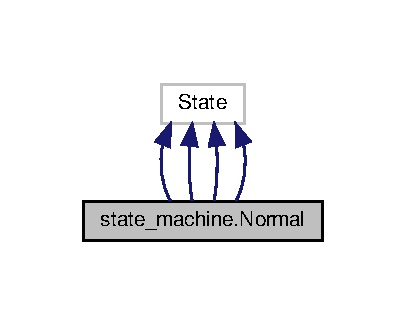
\includegraphics[width=195pt]{classstate__machine_1_1Normal__inherit__graph}
\end{center}
\end{figure}


Collaboration diagram for state\+\_\+machine.\+Normal\+:
\nopagebreak
\begin{figure}[H]
\begin{center}
\leavevmode
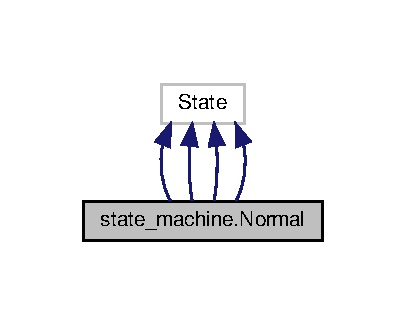
\includegraphics[width=195pt]{classstate__machine_1_1Normal__coll__graph}
\end{center}
\end{figure}
\subsection*{Public Member Functions}
\begin{DoxyCompactItemize}
\item 
\mbox{\Hypertarget{classstate__machine_1_1Normal_acdbc35a37d0350d7805a628048bc3bed}\label{classstate__machine_1_1Normal_acdbc35a37d0350d7805a628048bc3bed}} 
def \hyperlink{classstate__machine_1_1Normal_acdbc35a37d0350d7805a628048bc3bed}{\+\_\+\+\_\+init\+\_\+\+\_\+} (self)
\begin{DoxyCompactList}\small\item\em inizialization \end{DoxyCompactList}\item 
\mbox{\Hypertarget{classstate__machine_1_1Normal_a2930df5f4890ec4b47b2a8e18f9bff08}\label{classstate__machine_1_1Normal_a2930df5f4890ec4b47b2a8e18f9bff08}} 
def \hyperlink{classstate__machine_1_1Normal_a2930df5f4890ec4b47b2a8e18f9bff08}{execute} (self, userdata)
\begin{DoxyCompactList}\small\item\em execution \end{DoxyCompactList}\end{DoxyCompactItemize}
\subsection*{Public Attributes}
\begin{DoxyCompactItemize}
\item 
\hyperlink{classstate__machine_1_1Normal_af98201240ec5061a6b82b25758f6f207}{command}
\begin{DoxyCompactList}\small\item\em 2 outcomes defined \end{DoxyCompactList}\end{DoxyCompactItemize}


\subsection{Detailed Description}
\hyperlink{classstate__machine_1_1Normal}{Normal} state definition. 

Definition at line 282 of file state\+\_\+machine.\+py.



\subsection{Member Data Documentation}
\mbox{\Hypertarget{classstate__machine_1_1Normal_af98201240ec5061a6b82b25758f6f207}\label{classstate__machine_1_1Normal_af98201240ec5061a6b82b25758f6f207}} 
\index{state\+\_\+machine\+::\+Normal@{state\+\_\+machine\+::\+Normal}!command@{command}}
\index{command@{command}!state\+\_\+machine\+::\+Normal@{state\+\_\+machine\+::\+Normal}}
\subsubsection{\texorpdfstring{command}{command}}
{\footnotesize\ttfamily state\+\_\+machine.\+Normal.\+command}



2 outcomes defined 

switch in sleep state

command is sleep

read command (choice random between move random or go to sleep)

command is searchball 

Definition at line 288 of file state\+\_\+machine.\+py.



The documentation for this class was generated from the following file\+:\begin{DoxyCompactItemize}
\item 
/home/sara/catkin\+\_\+ws/src/exp\+\_\+assignment2/scripts/\hyperlink{state__machine_8py}{state\+\_\+machine.\+py}\end{DoxyCompactItemize}

\hypertarget{classstate__machine_1_1Play}{}\section{state\+\_\+machine.\+Play Class Reference}
\label{classstate__machine_1_1Play}\index{state\+\_\+machine.\+Play@{state\+\_\+machine.\+Play}}


\hyperlink{classstate__machine_1_1Play}{Play} state definition.  




Inheritance diagram for state\+\_\+machine.\+Play\+:
\nopagebreak
\begin{figure}[H]
\begin{center}
\leavevmode
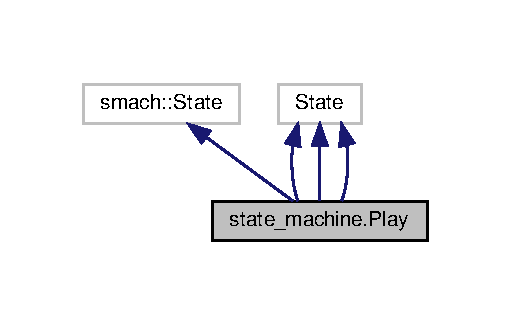
\includegraphics[width=245pt]{classstate__machine_1_1Play__inherit__graph}
\end{center}
\end{figure}


Collaboration diagram for state\+\_\+machine.\+Play\+:
\nopagebreak
\begin{figure}[H]
\begin{center}
\leavevmode
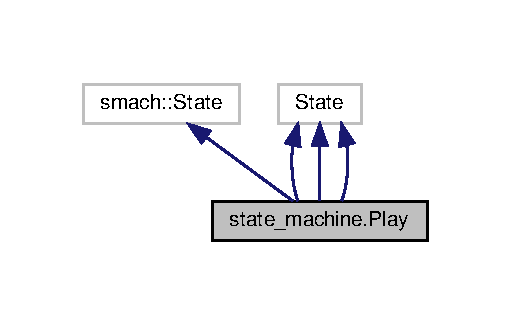
\includegraphics[width=245pt]{classstate__machine_1_1Play__coll__graph}
\end{center}
\end{figure}
\subsection*{Public Member Functions}
\begin{DoxyCompactItemize}
\item 
\mbox{\Hypertarget{classstate__machine_1_1Play_a5993a23d8be7f7b2647f71ede0334957}\label{classstate__machine_1_1Play_a5993a23d8be7f7b2647f71ede0334957}} 
def \hyperlink{classstate__machine_1_1Play_a5993a23d8be7f7b2647f71ede0334957}{\+\_\+\+\_\+init\+\_\+\+\_\+} (self)
\begin{DoxyCompactList}\small\item\em initialization \end{DoxyCompactList}\item 
\mbox{\Hypertarget{classstate__machine_1_1Play_a04168d6842960585b4bbcf58f950547b}\label{classstate__machine_1_1Play_a04168d6842960585b4bbcf58f950547b}} 
def \hyperlink{classstate__machine_1_1Play_a04168d6842960585b4bbcf58f950547b}{execute} (self, userdata)
\begin{DoxyCompactList}\small\item\em Execution. \end{DoxyCompactList}\item 
\mbox{\Hypertarget{classstate__machine_1_1Play_a5993a23d8be7f7b2647f71ede0334957}\label{classstate__machine_1_1Play_a5993a23d8be7f7b2647f71ede0334957}} 
def \hyperlink{classstate__machine_1_1Play_a5993a23d8be7f7b2647f71ede0334957}{\+\_\+\+\_\+init\+\_\+\+\_\+} (self)
\begin{DoxyCompactList}\small\item\em initialization \end{DoxyCompactList}\item 
\mbox{\Hypertarget{classstate__machine_1_1Play_a04168d6842960585b4bbcf58f950547b}\label{classstate__machine_1_1Play_a04168d6842960585b4bbcf58f950547b}} 
def \hyperlink{classstate__machine_1_1Play_a04168d6842960585b4bbcf58f950547b}{execute} (self, userdata)
\begin{DoxyCompactList}\small\item\em Execution. \end{DoxyCompactList}\item 
\mbox{\Hypertarget{classstate__machine_1_1Play_a5993a23d8be7f7b2647f71ede0334957}\label{classstate__machine_1_1Play_a5993a23d8be7f7b2647f71ede0334957}} 
def \hyperlink{classstate__machine_1_1Play_a5993a23d8be7f7b2647f71ede0334957}{\+\_\+\+\_\+init\+\_\+\+\_\+} (self)
\begin{DoxyCompactList}\small\item\em initialization \end{DoxyCompactList}\item 
\mbox{\Hypertarget{classstate__machine_1_1Play_a04168d6842960585b4bbcf58f950547b}\label{classstate__machine_1_1Play_a04168d6842960585b4bbcf58f950547b}} 
def \hyperlink{classstate__machine_1_1Play_a04168d6842960585b4bbcf58f950547b}{execute} (self, userdata)
\begin{DoxyCompactList}\small\item\em Execution. \end{DoxyCompactList}\item 
\mbox{\Hypertarget{classstate__machine_1_1Play_a5993a23d8be7f7b2647f71ede0334957}\label{classstate__machine_1_1Play_a5993a23d8be7f7b2647f71ede0334957}} 
def \hyperlink{classstate__machine_1_1Play_a5993a23d8be7f7b2647f71ede0334957}{\+\_\+\+\_\+init\+\_\+\+\_\+} (self)
\begin{DoxyCompactList}\small\item\em initialization \end{DoxyCompactList}\item 
\mbox{\Hypertarget{classstate__machine_1_1Play_a04168d6842960585b4bbcf58f950547b}\label{classstate__machine_1_1Play_a04168d6842960585b4bbcf58f950547b}} 
def \hyperlink{classstate__machine_1_1Play_a04168d6842960585b4bbcf58f950547b}{execute} (self, userdata)
\begin{DoxyCompactList}\small\item\em Execution. \end{DoxyCompactList}\end{DoxyCompactItemize}
\subsection*{Public Attributes}
\begin{DoxyCompactItemize}
\item 
\hyperlink{classstate__machine_1_1Play_ad451724fb1afb5a066901dead8566553}{angle\+\_\+pub}
\begin{DoxyCompactList}\small\item\em 1 outcome defined \+: \hyperlink{classstate__machine_1_1Normal}{Normal} \end{DoxyCompactList}\item 
\mbox{\Hypertarget{classstate__machine_1_1Play_a5817d2ff53ebb02ecf5ceea52ef97a94}\label{classstate__machine_1_1Play_a5817d2ff53ebb02ecf5ceea52ef97a94}} 
\hyperlink{classstate__machine_1_1Play_a5817d2ff53ebb02ecf5ceea52ef97a94}{location}
\begin{DoxyCompactList}\small\item\em 1 outcome defined \+: \hyperlink{classstate__machine_1_1Normal}{Normal} \end{DoxyCompactList}\item 
\mbox{\Hypertarget{classstate__machine_1_1Play_ad666be4461758154b1f51ddc979bca9b}\label{classstate__machine_1_1Play_ad666be4461758154b1f51ddc979bca9b}} 
{\bfseries Pointing\+Gesture}
\end{DoxyCompactItemize}


\subsection{Detailed Description}
\hyperlink{classstate__machine_1_1Play}{Play} state definition. 

Definition at line 359 of file state\+\_\+machine.\+py.



\subsection{Member Data Documentation}
\mbox{\Hypertarget{classstate__machine_1_1Play_ad451724fb1afb5a066901dead8566553}\label{classstate__machine_1_1Play_ad451724fb1afb5a066901dead8566553}} 
\index{state\+\_\+machine\+::\+Play@{state\+\_\+machine\+::\+Play}!angle\+\_\+pub@{angle\+\_\+pub}}
\index{angle\+\_\+pub@{angle\+\_\+pub}!state\+\_\+machine\+::\+Play@{state\+\_\+machine\+::\+Play}}
\subsubsection{\texorpdfstring{angle\+\_\+pub}{angle\_pub}}
{\footnotesize\ttfamily state\+\_\+machine.\+Play.\+angle\+\_\+pub}



1 outcome defined \+: \hyperlink{classstate__machine_1_1Normal}{Normal} 

publisher for move the head 

Definition at line 365 of file state\+\_\+machine.\+py.



The documentation for this class was generated from the following file\+:\begin{DoxyCompactItemize}
\item 
scripts/state\+\_\+machine.\+py\end{DoxyCompactItemize}

\hypertarget{classstate__machine_1_1Sleep}{}\section{state\+\_\+machine.\+Sleep Class Reference}
\label{classstate__machine_1_1Sleep}\index{state\+\_\+machine.\+Sleep@{state\+\_\+machine.\+Sleep}}


\hyperlink{classstate__machine_1_1Sleep}{Sleep} State definition.  




Inheritance diagram for state\+\_\+machine.\+Sleep\+:
\nopagebreak
\begin{figure}[H]
\begin{center}
\leavevmode
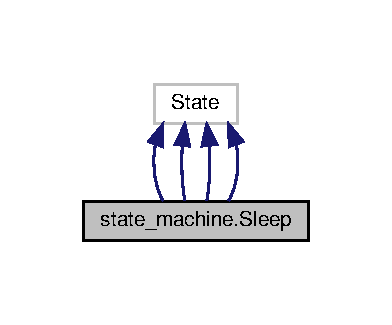
\includegraphics[width=188pt]{classstate__machine_1_1Sleep__inherit__graph}
\end{center}
\end{figure}


Collaboration diagram for state\+\_\+machine.\+Sleep\+:
\nopagebreak
\begin{figure}[H]
\begin{center}
\leavevmode
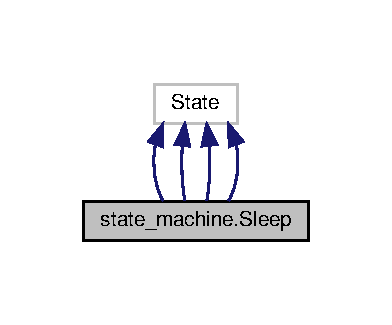
\includegraphics[width=188pt]{classstate__machine_1_1Sleep__coll__graph}
\end{center}
\end{figure}
\subsection*{Public Member Functions}
\begin{DoxyCompactItemize}
\item 
\mbox{\Hypertarget{classstate__machine_1_1Sleep_a473b93a1ddf11f9e664d1fb694ce1a3c}\label{classstate__machine_1_1Sleep_a473b93a1ddf11f9e664d1fb694ce1a3c}} 
def \hyperlink{classstate__machine_1_1Sleep_a473b93a1ddf11f9e664d1fb694ce1a3c}{\+\_\+\+\_\+init\+\_\+\+\_\+} (self)
\begin{DoxyCompactList}\small\item\em Initialization. \end{DoxyCompactList}\item 
\mbox{\Hypertarget{classstate__machine_1_1Sleep_a89527836f1edcefb6467fa9c041fbbfe}\label{classstate__machine_1_1Sleep_a89527836f1edcefb6467fa9c041fbbfe}} 
def \hyperlink{classstate__machine_1_1Sleep_a89527836f1edcefb6467fa9c041fbbfe}{execute} (self, userdata)
\begin{DoxyCompactList}\small\item\em Execution. \end{DoxyCompactList}\end{DoxyCompactItemize}


\subsection{Detailed Description}
\hyperlink{classstate__machine_1_1Sleep}{Sleep} State definition. 

Definition at line 340 of file state\+\_\+machine.\+py.



The documentation for this class was generated from the following file\+:\begin{DoxyCompactItemize}
\item 
/home/sara/catkin\+\_\+ws/src/exp\+\_\+assignment2/scripts/\hyperlink{state__machine_8py}{state\+\_\+machine.\+py}\end{DoxyCompactItemize}

\chapter{File Documentation}
\hypertarget{go__to__point__ball_8py}{}\section{/home/sara/catkin\+\_\+ws/src/exp\+\_\+assignment2/scripts/go\+\_\+to\+\_\+point\+\_\+ball.py File Reference}
\label{go__to__point__ball_8py}\index{/home/sara/catkin\+\_\+ws/src/exp\+\_\+assignment2/scripts/go\+\_\+to\+\_\+point\+\_\+ball.\+py@{/home/sara/catkin\+\_\+ws/src/exp\+\_\+assignment2/scripts/go\+\_\+to\+\_\+point\+\_\+ball.\+py}}


This node is actionlib server that permits to move the ball.  


\subsection*{Functions}
\begin{DoxyCompactItemize}
\item 
\mbox{\Hypertarget{go__to__point__ball_8py_a8b53c165c87e66822f50ab5daebc14dc}\label{go__to__point__ball_8py_a8b53c165c87e66822f50ab5daebc14dc}} 
def \hyperlink{go__to__point__ball_8py_a8b53c165c87e66822f50ab5daebc14dc}{go\+\_\+to\+\_\+point\+\_\+ball.\+clbk\+\_\+odom} (msg)
\begin{DoxyCompactList}\small\item\em Define callback. \end{DoxyCompactList}\item 
\mbox{\Hypertarget{go__to__point__ball_8py_ac5839fd3601d15749a1e1a28939b2c68}\label{go__to__point__ball_8py_ac5839fd3601d15749a1e1a28939b2c68}} 
def {\bfseries go\+\_\+to\+\_\+point\+\_\+ball.\+change\+\_\+state} (state)
\item 
\mbox{\Hypertarget{go__to__point__ball_8py_aecbf76a67251ff6a3a0840bb61e1c581}\label{go__to__point__ball_8py_aecbf76a67251ff6a3a0840bb61e1c581}} 
def \hyperlink{go__to__point__ball_8py_aecbf76a67251ff6a3a0840bb61e1c581}{go\+\_\+to\+\_\+point\+\_\+ball.\+go\+\_\+straight\+\_\+ahead} (des\+\_\+pos)
\begin{DoxyCompactList}\small\item\em define function to go straight \end{DoxyCompactList}\item 
\mbox{\Hypertarget{go__to__point__ball_8py_ab92c8b4240f09ff0b5d960c748ade799}\label{go__to__point__ball_8py_ab92c8b4240f09ff0b5d960c748ade799}} 
def \hyperlink{go__to__point__ball_8py_ab92c8b4240f09ff0b5d960c748ade799}{go\+\_\+to\+\_\+point\+\_\+ball.\+done} ()
\begin{DoxyCompactList}\small\item\em define function to stop when the goal is reached \end{DoxyCompactList}\item 
\mbox{\Hypertarget{go__to__point__ball_8py_ab0e05a6be4adc81f80b5635d9bd692d1}\label{go__to__point__ball_8py_ab0e05a6be4adc81f80b5635d9bd692d1}} 
def \hyperlink{go__to__point__ball_8py_ab0e05a6be4adc81f80b5635d9bd692d1}{go\+\_\+to\+\_\+point\+\_\+ball.\+planning} (goal)
\begin{DoxyCompactList}\small\item\em define planning funcion \end{DoxyCompactList}\item 
\mbox{\Hypertarget{go__to__point__ball_8py_a4d4c016b6bb12c612710a2d39ade3465}\label{go__to__point__ball_8py_a4d4c016b6bb12c612710a2d39ade3465}} 
def \hyperlink{go__to__point__ball_8py_a4d4c016b6bb12c612710a2d39ade3465}{go\+\_\+to\+\_\+point\+\_\+ball.\+main} ()
\begin{DoxyCompactList}\small\item\em Main function. \end{DoxyCompactList}\end{DoxyCompactItemize}
\subsection*{Variables}
\begin{DoxyCompactItemize}
\item 
\mbox{\Hypertarget{go__to__point__ball_8py_aa399e57145dd0af7eefcd5fab4174fe9}\label{go__to__point__ball_8py_aa399e57145dd0af7eefcd5fab4174fe9}} 
\hyperlink{go__to__point__ball_8py_aa399e57145dd0af7eefcd5fab4174fe9}{go\+\_\+to\+\_\+point\+\_\+ball.\+position\+\_\+} = Point()
\begin{DoxyCompactList}\small\item\em ball state variables \end{DoxyCompactList}\item 
\mbox{\Hypertarget{go__to__point__ball_8py_a03f1d8b257a2ae3d173a18c3fc2f8602}\label{go__to__point__ball_8py_a03f1d8b257a2ae3d173a18c3fc2f8602}} 
{\bfseries go\+\_\+to\+\_\+point\+\_\+ball.\+pose\+\_\+} = Pose()
\item 
\mbox{\Hypertarget{go__to__point__ball_8py_a74d8ca28c507d35baf1ea8e8f9595a78}\label{go__to__point__ball_8py_a74d8ca28c507d35baf1ea8e8f9595a78}} 
int {\bfseries go\+\_\+to\+\_\+point\+\_\+ball.\+yaw\+\_\+} = 0
\item 
\mbox{\Hypertarget{go__to__point__ball_8py_a0028df70b94b4041119cceba5e5aa79d}\label{go__to__point__ball_8py_a0028df70b94b4041119cceba5e5aa79d}} 
int \hyperlink{go__to__point__ball_8py_a0028df70b94b4041119cceba5e5aa79d}{go\+\_\+to\+\_\+point\+\_\+ball.\+state\+\_\+} = 0
\begin{DoxyCompactList}\small\item\em machine state \end{DoxyCompactList}\item 
\mbox{\Hypertarget{go__to__point__ball_8py_ac81a8393fb253c9e0b7255f779f16884}\label{go__to__point__ball_8py_ac81a8393fb253c9e0b7255f779f16884}} 
\hyperlink{go__to__point__ball_8py_ac81a8393fb253c9e0b7255f779f16884}{go\+\_\+to\+\_\+point\+\_\+ball.\+desired\+\_\+position\+\_\+} = Point()
\begin{DoxyCompactList}\small\item\em goal \end{DoxyCompactList}\item 
\mbox{\Hypertarget{go__to__point__ball_8py_acc228d72c1ee47a43061e3563ac20d5c}\label{go__to__point__ball_8py_acc228d72c1ee47a43061e3563ac20d5c}} 
int \hyperlink{go__to__point__ball_8py_acc228d72c1ee47a43061e3563ac20d5c}{go\+\_\+to\+\_\+point\+\_\+ball.\+yaw\+\_\+precision\+\_\+} = math.\+pi / 9
\begin{DoxyCompactList}\small\item\em parameters \end{DoxyCompactList}\item 
\mbox{\Hypertarget{go__to__point__ball_8py_a1985c69cf8534ba0bd2c6080f788a992}\label{go__to__point__ball_8py_a1985c69cf8534ba0bd2c6080f788a992}} 
int {\bfseries go\+\_\+to\+\_\+point\+\_\+ball.\+yaw\+\_\+precision\+\_\+2\+\_\+} = math.\+pi / 90
\item 
\mbox{\Hypertarget{go__to__point__ball_8py_a9a02c8ca89a09909111972ec4fd317ca}\label{go__to__point__ball_8py_a9a02c8ca89a09909111972ec4fd317ca}} 
float {\bfseries go\+\_\+to\+\_\+point\+\_\+ball.\+dist\+\_\+precision\+\_\+} = 0.\+1
\item 
\mbox{\Hypertarget{go__to__point__ball_8py_aac67ecb6c41141092b1ccaba4b537afc}\label{go__to__point__ball_8py_aac67ecb6c41141092b1ccaba4b537afc}} 
float {\bfseries go\+\_\+to\+\_\+point\+\_\+ball.\+kp\+\_\+a} = 3.\+0
\item 
\mbox{\Hypertarget{go__to__point__ball_8py_aeb49969b88b7ca77d9abdeae42cb1964}\label{go__to__point__ball_8py_aeb49969b88b7ca77d9abdeae42cb1964}} 
float {\bfseries go\+\_\+to\+\_\+point\+\_\+ball.\+kp\+\_\+d} = 0.\+5
\item 
\mbox{\Hypertarget{go__to__point__ball_8py_aa5173a26f3502ea035d7c563bbf1fb05}\label{go__to__point__ball_8py_aa5173a26f3502ea035d7c563bbf1fb05}} 
float {\bfseries go\+\_\+to\+\_\+point\+\_\+ball.\+ub\+\_\+a} = 0.\+6
\item 
\mbox{\Hypertarget{go__to__point__ball_8py_ae6440cb2a8ea6e8e7d2327cb4cd12dd3}\label{go__to__point__ball_8py_ae6440cb2a8ea6e8e7d2327cb4cd12dd3}} 
float {\bfseries go\+\_\+to\+\_\+point\+\_\+ball.\+lb\+\_\+a} = -\/0.\+5
\item 
\mbox{\Hypertarget{go__to__point__ball_8py_a1dabe6f24f898fa6f5303959917de757}\label{go__to__point__ball_8py_a1dabe6f24f898fa6f5303959917de757}} 
float {\bfseries go\+\_\+to\+\_\+point\+\_\+ball.\+ub\+\_\+d} = 2.\+0
\item 
\mbox{\Hypertarget{go__to__point__ball_8py_a176944c73499ce72fa754c7e1a6d138d}\label{go__to__point__ball_8py_a176944c73499ce72fa754c7e1a6d138d}} 
float {\bfseries go\+\_\+to\+\_\+point\+\_\+ball.\+z\+\_\+back} = 0.\+25
\item 
\mbox{\Hypertarget{go__to__point__ball_8py_a00b95c7141b558cd4466ca89d7c81640}\label{go__to__point__ball_8py_a00b95c7141b558cd4466ca89d7c81640}} 
\hyperlink{go__to__point__ball_8py_a00b95c7141b558cd4466ca89d7c81640}{go\+\_\+to\+\_\+point\+\_\+ball.\+pub} = None
\begin{DoxyCompactList}\small\item\em publisher \end{DoxyCompactList}\item 
\mbox{\Hypertarget{go__to__point__ball_8py_ae3016b9645d9bd2b863a34a30115a6af}\label{go__to__point__ball_8py_ae3016b9645d9bd2b863a34a30115a6af}} 
{\bfseries go\+\_\+to\+\_\+point\+\_\+ball.\+pubz} = None
\item 
\mbox{\Hypertarget{go__to__point__ball_8py_a9ac8c67ea55b320e5eb2bdf665173ffa}\label{go__to__point__ball_8py_a9ac8c67ea55b320e5eb2bdf665173ffa}} 
\hyperlink{go__to__point__ball_8py_a9ac8c67ea55b320e5eb2bdf665173ffa}{go\+\_\+to\+\_\+point\+\_\+ball.\+act\+\_\+s} = None
\begin{DoxyCompactList}\small\item\em action\+\_\+server \end{DoxyCompactList}\end{DoxyCompactItemize}


\subsection{Detailed Description}
This node is actionlib server that permits to move the ball. 


\hypertarget{go__to__point__robot_8py}{}\section{/home/sara/catkin\+\_\+ws/src/exp\+\_\+assignment2/scripts/go\+\_\+to\+\_\+point\+\_\+robot.py File Reference}
\label{go__to__point__robot_8py}\index{/home/sara/catkin\+\_\+ws/src/exp\+\_\+assignment2/scripts/go\+\_\+to\+\_\+point\+\_\+robot.\+py@{/home/sara/catkin\+\_\+ws/src/exp\+\_\+assignment2/scripts/go\+\_\+to\+\_\+point\+\_\+robot.\+py}}


This node is actionlib server that permits to move the robot.  


\subsection*{Functions}
\begin{DoxyCompactItemize}
\item 
\mbox{\Hypertarget{go__to__point__robot_8py_a03165218d1637827cb202d3df2d5c782}\label{go__to__point__robot_8py_a03165218d1637827cb202d3df2d5c782}} 
def \hyperlink{go__to__point__robot_8py_a03165218d1637827cb202d3df2d5c782}{go\+\_\+to\+\_\+point\+\_\+robot.\+clbk\+\_\+odom} (msg)
\begin{DoxyCompactList}\small\item\em Callback function. \end{DoxyCompactList}\item 
\mbox{\Hypertarget{go__to__point__robot_8py_a7dc82840479105130238b2bad7f4e927}\label{go__to__point__robot_8py_a7dc82840479105130238b2bad7f4e927}} 
def {\bfseries go\+\_\+to\+\_\+point\+\_\+robot.\+change\+\_\+state} (state)
\item 
\mbox{\Hypertarget{go__to__point__robot_8py_ae86d8ad9123b9ac0987b894814891c0e}\label{go__to__point__robot_8py_ae86d8ad9123b9ac0987b894814891c0e}} 
def \hyperlink{go__to__point__robot_8py_ae86d8ad9123b9ac0987b894814891c0e}{go\+\_\+to\+\_\+point\+\_\+robot.\+normalize\+\_\+angle} (angle)
\begin{DoxyCompactList}\small\item\em function to compute the norm \end{DoxyCompactList}\item 
\mbox{\Hypertarget{go__to__point__robot_8py_a3a0408db6b4459c8ac5f2c39b9751b1f}\label{go__to__point__robot_8py_a3a0408db6b4459c8ac5f2c39b9751b1f}} 
def {\bfseries go\+\_\+to\+\_\+point\+\_\+robot.\+fix\+\_\+yaw} (des\+\_\+pos)
\item 
\mbox{\Hypertarget{go__to__point__robot_8py_a573823369dd4b9399d01a500104204e1}\label{go__to__point__robot_8py_a573823369dd4b9399d01a500104204e1}} 
def \hyperlink{go__to__point__robot_8py_a573823369dd4b9399d01a500104204e1}{go\+\_\+to\+\_\+point\+\_\+robot.\+go\+\_\+straight\+\_\+ahead} (des\+\_\+pos)
\begin{DoxyCompactList}\small\item\em function to go straight \end{DoxyCompactList}\item 
\mbox{\Hypertarget{go__to__point__robot_8py_a1895554db4ca4e026a4e08012839beaf}\label{go__to__point__robot_8py_a1895554db4ca4e026a4e08012839beaf}} 
def \hyperlink{go__to__point__robot_8py_a1895554db4ca4e026a4e08012839beaf}{go\+\_\+to\+\_\+point\+\_\+robot.\+done} ()
\begin{DoxyCompactList}\small\item\em function to stop the robot when the goal is achieved \end{DoxyCompactList}\item 
\mbox{\Hypertarget{go__to__point__robot_8py_a06b798e382fdc93770464cbf5958726b}\label{go__to__point__robot_8py_a06b798e382fdc93770464cbf5958726b}} 
def \hyperlink{go__to__point__robot_8py_a06b798e382fdc93770464cbf5958726b}{go\+\_\+to\+\_\+point\+\_\+robot.\+planning} (goal)
\begin{DoxyCompactList}\small\item\em define planning funcion \end{DoxyCompactList}\item 
\mbox{\Hypertarget{go__to__point__robot_8py_a013e23353b468ecf925a25f3ec0ad0c3}\label{go__to__point__robot_8py_a013e23353b468ecf925a25f3ec0ad0c3}} 
def \hyperlink{go__to__point__robot_8py_a013e23353b468ecf925a25f3ec0ad0c3}{go\+\_\+to\+\_\+point\+\_\+robot.\+main} ()
\begin{DoxyCompactList}\small\item\em Main function. \end{DoxyCompactList}\end{DoxyCompactItemize}
\subsection*{Variables}
\begin{DoxyCompactItemize}
\item 
\mbox{\Hypertarget{go__to__point__robot_8py_acbca47166b9d5f046eaeadf1287f52c4}\label{go__to__point__robot_8py_acbca47166b9d5f046eaeadf1287f52c4}} 
\hyperlink{go__to__point__robot_8py_acbca47166b9d5f046eaeadf1287f52c4}{go\+\_\+to\+\_\+point\+\_\+robot.\+position\+\_\+} = Point()
\begin{DoxyCompactList}\small\item\em robot state variables \end{DoxyCompactList}\item 
\mbox{\Hypertarget{go__to__point__robot_8py_a9ac7f45f0d64cf9ef7666d1f825ef9ba}\label{go__to__point__robot_8py_a9ac7f45f0d64cf9ef7666d1f825ef9ba}} 
{\bfseries go\+\_\+to\+\_\+point\+\_\+robot.\+pose\+\_\+} = Pose()
\item 
\mbox{\Hypertarget{go__to__point__robot_8py_af0544cdffc791a807b9062c979cf0c3d}\label{go__to__point__robot_8py_af0544cdffc791a807b9062c979cf0c3d}} 
int {\bfseries go\+\_\+to\+\_\+point\+\_\+robot.\+yaw\+\_\+} = 0
\item 
\mbox{\Hypertarget{go__to__point__robot_8py_a68762504c0683adedb89a8f7d431f475}\label{go__to__point__robot_8py_a68762504c0683adedb89a8f7d431f475}} 
int \hyperlink{go__to__point__robot_8py_a68762504c0683adedb89a8f7d431f475}{go\+\_\+to\+\_\+point\+\_\+robot.\+state\+\_\+} = 0
\begin{DoxyCompactList}\small\item\em machine state \end{DoxyCompactList}\item 
\mbox{\Hypertarget{go__to__point__robot_8py_ab42eca5c5072ff7b4d95c8e13827dba7}\label{go__to__point__robot_8py_ab42eca5c5072ff7b4d95c8e13827dba7}} 
\hyperlink{go__to__point__robot_8py_ab42eca5c5072ff7b4d95c8e13827dba7}{go\+\_\+to\+\_\+point\+\_\+robot.\+desired\+\_\+position\+\_\+} = Point()
\begin{DoxyCompactList}\small\item\em goal \end{DoxyCompactList}\item 
\mbox{\Hypertarget{go__to__point__robot_8py_ad3b22a785c833ad2cdd10712a66f11c8}\label{go__to__point__robot_8py_ad3b22a785c833ad2cdd10712a66f11c8}} 
{\bfseries go\+\_\+to\+\_\+point\+\_\+robot.\+z}
\item 
\mbox{\Hypertarget{go__to__point__robot_8py_ad0131301589fb7d3d9462cff81932fcf}\label{go__to__point__robot_8py_ad0131301589fb7d3d9462cff81932fcf}} 
int \hyperlink{go__to__point__robot_8py_ad0131301589fb7d3d9462cff81932fcf}{go\+\_\+to\+\_\+point\+\_\+robot.\+yaw\+\_\+precision\+\_\+} = math.\+pi / 9
\begin{DoxyCompactList}\small\item\em parameters \end{DoxyCompactList}\item 
\mbox{\Hypertarget{go__to__point__robot_8py_aadcca20dfdd8e843623186e6efde0481}\label{go__to__point__robot_8py_aadcca20dfdd8e843623186e6efde0481}} 
int {\bfseries go\+\_\+to\+\_\+point\+\_\+robot.\+yaw\+\_\+precision\+\_\+2\+\_\+} = math.\+pi / 90
\item 
\mbox{\Hypertarget{go__to__point__robot_8py_adce474cb3bcc2782904a1e6129217a4c}\label{go__to__point__robot_8py_adce474cb3bcc2782904a1e6129217a4c}} 
float {\bfseries go\+\_\+to\+\_\+point\+\_\+robot.\+dist\+\_\+precision\+\_\+} = 0.\+1
\item 
\mbox{\Hypertarget{go__to__point__robot_8py_ab9bae8b08a7c50f11e55e3fae44f7777}\label{go__to__point__robot_8py_ab9bae8b08a7c50f11e55e3fae44f7777}} 
float {\bfseries go\+\_\+to\+\_\+point\+\_\+robot.\+kp\+\_\+a} = -\/3.\+0
\item 
\mbox{\Hypertarget{go__to__point__robot_8py_afaac446f10588cd97bfda3bf31c3b670}\label{go__to__point__robot_8py_afaac446f10588cd97bfda3bf31c3b670}} 
float {\bfseries go\+\_\+to\+\_\+point\+\_\+robot.\+kp\+\_\+d} = 0.\+2
\item 
\mbox{\Hypertarget{go__to__point__robot_8py_a82aa92171409b5a766ecc7ec77f1488f}\label{go__to__point__robot_8py_a82aa92171409b5a766ecc7ec77f1488f}} 
float {\bfseries go\+\_\+to\+\_\+point\+\_\+robot.\+ub\+\_\+a} = 0.\+6
\item 
\mbox{\Hypertarget{go__to__point__robot_8py_a0a5daf54d4f98b8898f69fc331bcc1f0}\label{go__to__point__robot_8py_a0a5daf54d4f98b8898f69fc331bcc1f0}} 
float {\bfseries go\+\_\+to\+\_\+point\+\_\+robot.\+lb\+\_\+a} = -\/0.\+5
\item 
\mbox{\Hypertarget{go__to__point__robot_8py_aa54f25328ab1ea2787c879431057298f}\label{go__to__point__robot_8py_aa54f25328ab1ea2787c879431057298f}} 
float {\bfseries go\+\_\+to\+\_\+point\+\_\+robot.\+ub\+\_\+d} = 0.\+6
\item 
\mbox{\Hypertarget{go__to__point__robot_8py_aa3df6e395e3d2ee11f4f87c88bde46bb}\label{go__to__point__robot_8py_aa3df6e395e3d2ee11f4f87c88bde46bb}} 
float {\bfseries go\+\_\+to\+\_\+point\+\_\+robot.\+z\+\_\+back} = 0.\+25
\item 
\mbox{\Hypertarget{go__to__point__robot_8py_a6e68302a4efb615222a73c01f4ea514e}\label{go__to__point__robot_8py_a6e68302a4efb615222a73c01f4ea514e}} 
\hyperlink{go__to__point__robot_8py_a6e68302a4efb615222a73c01f4ea514e}{go\+\_\+to\+\_\+point\+\_\+robot.\+pub} = None
\begin{DoxyCompactList}\small\item\em publisher \end{DoxyCompactList}\item 
\mbox{\Hypertarget{go__to__point__robot_8py_ab0db118eb85d7bb034dfb80210d478be}\label{go__to__point__robot_8py_ab0db118eb85d7bb034dfb80210d478be}} 
{\bfseries go\+\_\+to\+\_\+point\+\_\+robot.\+pubz} = None
\item 
\mbox{\Hypertarget{go__to__point__robot_8py_ab19ed2eba072e150275e059ca41a4cfc}\label{go__to__point__robot_8py_ab19ed2eba072e150275e059ca41a4cfc}} 
\hyperlink{go__to__point__robot_8py_ab19ed2eba072e150275e059ca41a4cfc}{go\+\_\+to\+\_\+point\+\_\+robot.\+act\+\_\+s} = None
\begin{DoxyCompactList}\small\item\em action\+\_\+server \end{DoxyCompactList}\end{DoxyCompactItemize}


\subsection{Detailed Description}
This node is actionlib server that permits to move the robot. 


\hypertarget{move__ball__around_8py}{}\section{/home/sara/catkin\+\_\+ws/src/exp\+\_\+assignment2/scripts/move\+\_\+ball\+\_\+around.py File Reference}
\label{move__ball__around_8py}\index{/home/sara/catkin\+\_\+ws/src/exp\+\_\+assignment2/scripts/move\+\_\+ball\+\_\+around.\+py@{/home/sara/catkin\+\_\+ws/src/exp\+\_\+assignment2/scripts/move\+\_\+ball\+\_\+around.\+py}}


This node permits to the ball to move around, wait for a while and disappear.  


\subsection*{Functions}
\begin{DoxyCompactItemize}
\item 
\mbox{\Hypertarget{move__ball__around_8py_a6671388c0025baa6165d1dfbb17b91a7}\label{move__ball__around_8py_a6671388c0025baa6165d1dfbb17b91a7}} 
def \hyperlink{move__ball__around_8py_a6671388c0025baa6165d1dfbb17b91a7}{move\+\_\+ball\+\_\+around.\+move\+\_\+ball} (target)
\begin{DoxyCompactList}\small\item\em client of actionlib server for moving the ball \end{DoxyCompactList}\item 
\mbox{\Hypertarget{move__ball__around_8py_ab8a5a225b98899a5b5cac85bdb22ce33}\label{move__ball__around_8py_ab8a5a225b98899a5b5cac85bdb22ce33}} 
def \hyperlink{move__ball__around_8py_ab8a5a225b98899a5b5cac85bdb22ce33}{move\+\_\+ball\+\_\+around.\+main} ()
\begin{DoxyCompactList}\small\item\em Main function. \end{DoxyCompactList}\end{DoxyCompactItemize}


\subsection{Detailed Description}
This node permits to the ball to move around, wait for a while and disappear. 


\hypertarget{state__machine_8py}{}\section{/home/sara/catkin\+\_\+ws/src/exp\+\_\+assignment2/scripts/state\+\_\+machine.py File Reference}
\label{state__machine_8py}\index{/home/sara/catkin\+\_\+ws/src/exp\+\_\+assignment2/scripts/state\+\_\+machine.\+py@{/home/sara/catkin\+\_\+ws/src/exp\+\_\+assignment2/scripts/state\+\_\+machine.\+py}}


This node implements a state machine which permits to move around and to search for a ball, go to sleep, and play with the ball when the last one is found.  


\subsection*{Classes}
\begin{DoxyCompactItemize}
\item 
class \hyperlink{classstate__machine_1_1image__feature}{state\+\_\+machine.\+image\+\_\+feature}
\begin{DoxyCompactList}\small\item\em Istance called in play state to track the ball. \end{DoxyCompactList}\item 
class \hyperlink{classstate__machine_1_1Normal}{state\+\_\+machine.\+Normal}
\begin{DoxyCompactList}\small\item\em \hyperlink{classstate__machine_1_1Normal}{Normal} state definition. \end{DoxyCompactList}\item 
class \hyperlink{classstate__machine_1_1Sleep}{state\+\_\+machine.\+Sleep}
\begin{DoxyCompactList}\small\item\em \hyperlink{classstate__machine_1_1Sleep}{Sleep} State definition. \end{DoxyCompactList}\item 
class \hyperlink{classstate__machine_1_1Play}{state\+\_\+machine.\+Play}
\begin{DoxyCompactList}\small\item\em \hyperlink{classstate__machine_1_1Play}{Play} state definition. \end{DoxyCompactList}\end{DoxyCompactItemize}
\subsection*{Functions}
\begin{DoxyCompactItemize}
\item 
\mbox{\Hypertarget{state__machine_8py_afaa99f0eebff6571a958fcc827c6a367}\label{state__machine_8py_afaa99f0eebff6571a958fcc827c6a367}} 
def \hyperlink{state__machine_8py_afaa99f0eebff6571a958fcc827c6a367}{state\+\_\+machine.\+user\+\_\+action} ()
\begin{DoxyCompactList}\small\item\em User Action function. \end{DoxyCompactList}\item 
\mbox{\Hypertarget{state__machine_8py_a0a97a0736d651ef180460288b1f49d5d}\label{state__machine_8py_a0a97a0736d651ef180460288b1f49d5d}} 
def \hyperlink{state__machine_8py_a0a97a0736d651ef180460288b1f49d5d}{state\+\_\+machine.\+move\+\_\+dog} (target)
\begin{DoxyCompactList}\small\item\em client of actionlib server for moving the dog robot \end{DoxyCompactList}\item 
def \hyperlink{state__machine_8py_a1db226061483cf9f83c8a5e4003ab0c7}{state\+\_\+machine.\+Normal\+\_\+clbk} (ros\+\_\+data)
\begin{DoxyCompactList}\small\item\em Callback for \hyperlink{classstate__machine_1_1Normal}{Normal} State for subscribe to a Camera1 \+: it checks if the ball is on the arena, if it is, a parameter (Detected\+Ball) becomes 1 and the robot goes to play, otherwise the parameter becomes 0 and the robot moves randomly. \end{DoxyCompactList}\item 
\mbox{\Hypertarget{state__machine_8py_a5c680ce705e6052fa07c6cece21743d0}\label{state__machine_8py_a5c680ce705e6052fa07c6cece21743d0}} 
def \hyperlink{state__machine_8py_a5c680ce705e6052fa07c6cece21743d0}{state\+\_\+machine.\+main} ()
\begin{DoxyCompactList}\small\item\em Main Function definition. \end{DoxyCompactList}\end{DoxyCompactItemize}
\subsection*{Variables}
\begin{DoxyCompactItemize}
\item 
\mbox{\Hypertarget{state__machine_8py_a8b1913f94c64745cffa6fd2062e38f74}\label{state__machine_8py_a8b1913f94c64745cffa6fd2062e38f74}} 
bool {\bfseries state\+\_\+machine.\+V\+E\+R\+B\+O\+SE} = False
\item 
\mbox{\Hypertarget{state__machine_8py_a54f86ff7d2cdd140c50ebb96450702e7}\label{state__machine_8py_a54f86ff7d2cdd140c50ebb96450702e7}} 
{\bfseries state\+\_\+machine.\+vel} = Twist()
\item 
\mbox{\Hypertarget{state__machine_8py_a16809bbff85c893ec571a4a74e7e7527}\label{state__machine_8py_a16809bbff85c893ec571a4a74e7e7527}} 
{\bfseries state\+\_\+machine.\+angle\+\_\+camera} = Float64()
\item 
\hyperlink{state__machine_8py_af9be804204216b5a8fbe5121cf1ab55c}{state\+\_\+machine.\+image\+\_\+pub}
\begin{DoxyCompactList}\small\item\em Publisher. \end{DoxyCompactList}\item 
\mbox{\Hypertarget{state__machine_8py_a552cb14a092a4c44a3092b286def2ec4}\label{state__machine_8py_a552cb14a092a4c44a3092b286def2ec4}} 
{\bfseries state\+\_\+machine.\+vel\+\_\+pub} = rospy.\+Publisher(\char`\"{}/robot/cmd\+\_\+vel\char`\"{}, Twist, queue\+\_\+size=1)
\end{DoxyCompactItemize}


\subsection{Detailed Description}
This node implements a state machine which permits to move around and to search for a ball, go to sleep, and play with the ball when the last one is found. 



\subsection{Function Documentation}
\mbox{\Hypertarget{state__machine_8py_file_a1db226061483cf9f83c8a5e4003ab0c7}\label{state__machine_8py_file_a1db226061483cf9f83c8a5e4003ab0c7}} 
\index{state\+\_\+machine.\+py@{state\+\_\+machine.\+py}!Normal\+\_\+clbk@{Normal\+\_\+clbk}}
\index{Normal\+\_\+clbk@{Normal\+\_\+clbk}!state\+\_\+machine.\+py@{state\+\_\+machine.\+py}}
\subsubsection{\texorpdfstring{Normal\+\_\+clbk()}{Normal\_clbk()}}
{\footnotesize\ttfamily def state\+\_\+machine.\+Normal\+\_\+clbk (\begin{DoxyParamCaption}\item[{}]{ros\+\_\+data }\end{DoxyParamCaption})}



Callback for Normal State for subscribe to a Camera1 \+: it checks if the ball is on the arena, if it is, a parameter (Detected\+Ball) becomes 1 and the robot goes to play, otherwise the parameter becomes 0 and the robot moves randomly. 



Definition at line 97 of file state\+\_\+machine.\+py.


\begin{DoxyCode}
97 \textcolor{keyword}{def }Normal\_clbk(ros\_data): 
98     
99     \textcolor{keyword}{global} count2
100     \textcolor{keyword}{global} DetectedBall
101     \textcolor{keyword}{global} SearchBallSub
102 
103     \textcolor{keywordflow}{while} rospy.get\_param(\textcolor{stringliteral}{'count2'}) == 360: 
104         time.sleep(1) 
105 
106     
107     
108     np\_arr = np.fromstring(ros\_data.data, np.uint8)
109     image\_np = cv2.imdecode(np\_arr, cv2.IMREAD\_COLOR)  \textcolor{comment}{# OpenCV >= 3.0:}
110     
111     greenLower = (50, 50, 20)
112     greenUpper = (70, 255, 255)
113     
114     blurred = cv2.GaussianBlur(image\_np, (11, 11), 0)
115     hsv = cv2.cvtColor(blurred, cv2.COLOR\_BGR2HSV)
116     mask = cv2.inRange(hsv, greenLower, greenUpper)
117     mask = cv2.erode(mask, \textcolor{keywordtype}{None}, iterations=2)
118     mask = cv2.dilate(mask, \textcolor{keywordtype}{None}, iterations=2)
119 
120     
121     cnts = cv2.findContours(mask.copy(), cv2.RETR\_EXTERNAL,
122                             cv2.CHAIN\_APPROX\_SIMPLE)
123     cnts = imutils.grab\_contours(cnts)
124     center = \textcolor{keywordtype}{None}
125 
126 
127 
128     
129 
130     \textcolor{keywordflow}{if} len(cnts) > 0:
131         c = max(cnts, key=cv2.contourArea)
132         ((x, y), radius) = cv2.minEnclosingCircle(c)
133         M = cv2.moments(c)
134         center = (int(M[\textcolor{stringliteral}{"m10"}] / M[\textcolor{stringliteral}{"m00"}]), int(M[\textcolor{stringliteral}{"m01"}] / M[\textcolor{stringliteral}{"m00"}]))
135 
136         
137         \textcolor{keywordflow}{if} radius > 10:
138             
139 
140             cv2.circle(image\_np, (int(x), int(y)), int(radius),
141                         (0, 255, 255), 2)
142             cv2.circle(image\_np, center, 5, (0, 0, 255), -1)
143 
144             
145             rospy.set\_param(\textcolor{stringliteral}{'DetectedBall'},1)  
146 
147     
148     \textcolor{keywordflow}{else}:
149 
150         vel\_ = Twist()
151         
152         vel\_.angular.z = 0.5 
153         vel\_pub.publish(vel\_) 
154         count2 = rospy.get\_param(\textcolor{stringliteral}{'count2'})
155         count2 = count2 + 1 
156         rospy.set\_param(\textcolor{stringliteral}{'count2'}, count2) 
157           
158 
159     
160     cv2.imshow(\textcolor{stringliteral}{'window'}, image\_np)
161     cv2.waitKey(2)
162          
163 
164 
\end{DoxyCode}


\subsection{Variable Documentation}
\mbox{\Hypertarget{state__machine_8py_file_af9be804204216b5a8fbe5121cf1ab55c}\label{state__machine_8py_file_af9be804204216b5a8fbe5121cf1ab55c}} 
\index{state\+\_\+machine.\+py@{state\+\_\+machine.\+py}!image\+\_\+pub@{image\+\_\+pub}}
\index{image\+\_\+pub@{image\+\_\+pub}!state\+\_\+machine.\+py@{state\+\_\+machine.\+py}}
\subsubsection{\texorpdfstring{image\+\_\+pub}{image\_pub}}
{\footnotesize\ttfamily state\+\_\+machine.\+image\+\_\+pub}

{\bfseries Initial value\+:}
\begin{DoxyCode}
1 =  rospy.Publisher(\textcolor{stringliteral}{"/output/image\_raw/compressed"},
2                                          CompressedImage, queue\_size=1)
\end{DoxyCode}


Publisher. 



Definition at line 90 of file state\+\_\+machine.\+py.


%--- End generated contents ---

% Index
\backmatter
\newpage
\phantomsection
\clearemptydoublepage
\addcontentsline{toc}{chapter}{Index}
\printindex

\end{document}
